\documentclass[twoside]{book}

% Packages required by doxygen
\usepackage{fixltx2e}
\usepackage{calc}
\usepackage{doxygen}
\usepackage[export]{adjustbox} % also loads graphicx
\usepackage{graphicx}
\usepackage[utf8]{inputenc}
\usepackage{makeidx}
\usepackage{multicol}
\usepackage{multirow}
\PassOptionsToPackage{warn}{textcomp}
\usepackage{textcomp}
\usepackage[nointegrals]{wasysym}
\usepackage[table]{xcolor}

% Font selection
\usepackage[T1]{fontenc}
\usepackage[scaled=.90]{helvet}
\usepackage{courier}
\usepackage{amssymb}
\usepackage{sectsty}
\renewcommand{\familydefault}{\sfdefault}
\allsectionsfont{%
  \fontseries{bc}\selectfont%
  \color{darkgray}%
}
\renewcommand{\DoxyLabelFont}{%
  \fontseries{bc}\selectfont%
  \color{darkgray}%
}
\newcommand{\+}{\discretionary{\mbox{\scriptsize$\hookleftarrow$}}{}{}}

% Page & text layout
\usepackage{geometry}
\geometry{%
  a4paper,%
  top=2.5cm,%
  bottom=2.5cm,%
  left=2.5cm,%
  right=2.5cm%
}
\tolerance=750
\hfuzz=15pt
\hbadness=750
\setlength{\emergencystretch}{15pt}
\setlength{\parindent}{0cm}
\setlength{\parskip}{3ex plus 2ex minus 2ex}
\makeatletter
\renewcommand{\paragraph}{%
  \@startsection{paragraph}{4}{0ex}{-1.0ex}{1.0ex}{%
    \normalfont\normalsize\bfseries\SS@parafont%
  }%
}
\renewcommand{\subparagraph}{%
  \@startsection{subparagraph}{5}{0ex}{-1.0ex}{1.0ex}{%
    \normalfont\normalsize\bfseries\SS@subparafont%
  }%
}
\makeatother

% Headers & footers
\usepackage{fancyhdr}
\pagestyle{fancyplain}
\fancyhead[LE]{\fancyplain{}{\bfseries\thepage}}
\fancyhead[CE]{\fancyplain{}{}}
\fancyhead[RE]{\fancyplain{}{\bfseries\leftmark}}
\fancyhead[LO]{\fancyplain{}{\bfseries\rightmark}}
\fancyhead[CO]{\fancyplain{}{}}
\fancyhead[RO]{\fancyplain{}{\bfseries\thepage}}
\fancyfoot[LE]{\fancyplain{}{}}
\fancyfoot[CE]{\fancyplain{}{}}
\fancyfoot[RE]{\fancyplain{}{\bfseries\scriptsize Generated by Doxygen }}
\fancyfoot[LO]{\fancyplain{}{\bfseries\scriptsize Generated by Doxygen }}
\fancyfoot[CO]{\fancyplain{}{}}
\fancyfoot[RO]{\fancyplain{}{}}
\renewcommand{\footrulewidth}{0.4pt}
\renewcommand{\chaptermark}[1]{%
  \markboth{#1}{}%
}
\renewcommand{\sectionmark}[1]{%
  \markright{\thesection\ #1}%
}

% Indices & bibliography
\usepackage{natbib}
\usepackage[titles]{tocloft}
\setcounter{tocdepth}{3}
\setcounter{secnumdepth}{5}
\makeindex

% Hyperlinks (required, but should be loaded last)
\usepackage{ifpdf}
\ifpdf
  \usepackage[pdftex,pagebackref=true]{hyperref}
\else
  \usepackage[ps2pdf,pagebackref=true]{hyperref}
\fi
\hypersetup{%
  colorlinks=true,%
  linkcolor=blue,%
  citecolor=blue,%
  unicode%
}

% Custom commands
\newcommand{\clearemptydoublepage}{%
  \newpage{\pagestyle{empty}\cleardoublepage}%
}

\usepackage{caption}
\captionsetup{labelsep=space,justification=centering,font={bf},singlelinecheck=off,skip=4pt,position=top}

%===== C O N T E N T S =====

\begin{document}

% Titlepage & ToC
\hypersetup{pageanchor=false,
             bookmarksnumbered=true,
             pdfencoding=unicode
            }
\pagenumbering{alph}
\begin{titlepage}
\vspace*{7cm}
\begin{center}%
{\Large Evm virtual machine \\[1ex]\large 1 }\\
\vspace*{1cm}
{\large Generated by Doxygen 1.8.14}\\
\end{center}
\end{titlepage}
\clearemptydoublepage
\pagenumbering{roman}
\tableofcontents
\clearemptydoublepage
\pagenumbering{arabic}
\hypersetup{pageanchor=true}

%--- Begin generated contents ---
\chapter{Namespace Index}
\section{Namespace List}
Here is a list of all documented namespaces with brief descriptions\+:\begin{DoxyCompactList}
\item\contentsline{section}{\mbox{\hyperlink{namespace_eva}{Eva}} }{\pageref{namespace_eva}}{}
\item\contentsline{section}{\mbox{\hyperlink{namespace_evm}{Evm}} }{\pageref{namespace_evm}}{}
\item\contentsline{section}{\mbox{\hyperlink{namespace_operation}{Operation}} }{\pageref{namespace_operation}}{}
\end{DoxyCompactList}

\chapter{Hierarchical Index}
\section{Class Hierarchy}
This inheritance list is sorted roughly, but not completely, alphabetically\+:\begin{DoxyCompactList}
\item \contentsline{section}{Evm\+:\+:Application}{\pageref{struct_evm_1_1_application}}{}
\item \contentsline{section}{Evm\+:\+:Utils\+:\+:Bit\+Buffer}{\pageref{struct_evm_1_1_utils_1_1_bit_buffer}}{}
\item \contentsline{section}{Evm\+:\+:Cli\+Configuration}{\pageref{struct_evm_1_1_cli_configuration}}{}
\item \contentsline{section}{Evm\+:\+:Argument\+:\+:Convert\+Union}{\pageref{union_evm_1_1_argument_1_1_convert_union}}{}
\item \contentsline{section}{Evm\+:\+:File\+:\+:Evm\+File}{\pageref{struct_evm_1_1_file_1_1_evm_file}}{}
\item \contentsline{section}{Evm\+:\+:File\+:\+:Evm\+File\+:\+:Header}{\pageref{struct_evm_1_1_file_1_1_evm_file_1_1_header}}{}
\item \contentsline{section}{Evm\+:\+:Argument\+:\+:I\+Argument}{\pageref{struct_evm_1_1_argument_1_1_i_argument}}{}
\begin{DoxyCompactList}
\item \contentsline{section}{Evm\+:\+:Argument\+:\+:Address\+Argument}{\pageref{struct_evm_1_1_argument_1_1_address_argument}}{}
\item \contentsline{section}{Evm\+:\+:Argument\+:\+:Const\+Argument}{\pageref{struct_evm_1_1_argument_1_1_const_argument}}{}
\item \contentsline{section}{Evm\+:\+:Argument\+:\+:I\+Register\+Base\+Argument}{\pageref{struct_evm_1_1_argument_1_1_i_register_base_argument}}{}
\begin{DoxyCompactList}
\item \contentsline{section}{Evm\+:\+:Argument\+:\+:Memory\+B\+Y\+T\+E\+Argument}{\pageref{struct_evm_1_1_argument_1_1_memory_b_y_t_e_argument}}{}
\item \contentsline{section}{Evm\+:\+:Argument\+:\+:Memory\+D\+W\+O\+R\+D\+Argument}{\pageref{struct_evm_1_1_argument_1_1_memory_d_w_o_r_d_argument}}{}
\item \contentsline{section}{Evm\+:\+:Argument\+:\+:Memory\+Q\+W\+O\+R\+D\+Argument}{\pageref{struct_evm_1_1_argument_1_1_memory_q_w_o_r_d_argument}}{}
\item \contentsline{section}{Evm\+:\+:Argument\+:\+:Memory\+W\+O\+R\+D\+Argument}{\pageref{struct_evm_1_1_argument_1_1_memory_w_o_r_d_argument}}{}
\item \contentsline{section}{Evm\+:\+:Argument\+:\+:Register\+Argument}{\pageref{struct_evm_1_1_argument_1_1_register_argument}}{}
\end{DoxyCompactList}
\end{DoxyCompactList}
\item \contentsline{section}{Evm\+:\+:Operation\+:\+:I\+Operation}{\pageref{struct_evm_1_1_operation_1_1_i_operation}}{}
\begin{DoxyCompactList}
\item \contentsline{section}{Evm\+:\+:Operation\+:\+:Call\+Operation}{\pageref{struct_evm_1_1_operation_1_1_call_operation}}{}
\item \contentsline{section}{Evm\+:\+:Operation\+:\+:Console\+Read\+Operation}{\pageref{struct_evm_1_1_operation_1_1_console_read_operation}}{}
\item \contentsline{section}{Evm\+:\+:Operation\+:\+:Console\+Write\+Operation}{\pageref{struct_evm_1_1_operation_1_1_console_write_operation}}{}
\item \contentsline{section}{Evm\+:\+:Operation\+:\+:Create\+Thread\+Operation}{\pageref{struct_evm_1_1_operation_1_1_create_thread_operation}}{}
\item \contentsline{section}{Evm\+:\+:Operation\+:\+:Hlt\+Operation}{\pageref{struct_evm_1_1_operation_1_1_hlt_operation}}{}
\item \contentsline{section}{Evm\+:\+:Operation\+:\+:Join\+Operation}{\pageref{struct_evm_1_1_operation_1_1_join_operation}}{}
\item \contentsline{section}{Evm\+:\+:Operation\+:\+:Jump\+Equal\+Operation}{\pageref{struct_evm_1_1_operation_1_1_jump_equal_operation}}{}
\item \contentsline{section}{Evm\+:\+:Operation\+:\+:Jump\+Operation}{\pageref{struct_evm_1_1_operation_1_1_jump_operation}}{}
\item \contentsline{section}{Evm\+:\+:Operation\+:\+:Load\+Const\+Operation}{\pageref{struct_evm_1_1_operation_1_1_load_const_operation}}{}
\item \contentsline{section}{Evm\+:\+:Operation\+:\+:Lock\+Operation}{\pageref{struct_evm_1_1_operation_1_1_lock_operation}}{}
\item \contentsline{section}{Evm\+:\+:Operation\+:\+:Math\+Operation}{\pageref{struct_evm_1_1_operation_1_1_math_operation}}{}
\item \contentsline{section}{Evm\+:\+:Operation\+:\+:Mov\+Operation}{\pageref{struct_evm_1_1_operation_1_1_mov_operation}}{}
\item \contentsline{section}{Evm\+:\+:Operation\+:\+:Read\+Operation}{\pageref{struct_evm_1_1_operation_1_1_read_operation}}{}
\item \contentsline{section}{Evm\+:\+:Operation\+:\+:Ret\+Operation}{\pageref{struct_evm_1_1_operation_1_1_ret_operation}}{}
\item \contentsline{section}{Evm\+:\+:Operation\+:\+:Sleep\+Operation}{\pageref{struct_evm_1_1_operation_1_1_sleep_operation}}{}
\item \contentsline{section}{Evm\+:\+:Operation\+:\+:Unlock\+Operation}{\pageref{struct_evm_1_1_operation_1_1_unlock_operation}}{}
\item \contentsline{section}{Evm\+:\+:Operation\+:\+:Write\+Operation}{\pageref{struct_evm_1_1_operation_1_1_write_operation}}{}
\end{DoxyCompactList}
\item \contentsline{section}{Evm\+:\+:Operation\+:\+:I\+Operation\+Factory}{\pageref{struct_evm_1_1_operation_1_1_i_operation_factory}}{}
\begin{DoxyCompactList}
\item \contentsline{section}{Evm\+:\+:Operation\+:\+:Address\+Operation\+Factory$<$ T $>$}{\pageref{struct_evm_1_1_operation_1_1_address_operation_factory}}{}
\item \contentsline{section}{Evm\+:\+:Operation\+:\+:Arg1\+Arg2\+Arg3\+Arg4\+Operation\+Factory$<$ T $>$}{\pageref{struct_evm_1_1_operation_1_1_arg1_arg2_arg3_arg4_operation_factory}}{}
\item \contentsline{section}{Evm\+:\+:Operation\+:\+:Arg1\+Arg2\+Arg3\+Operation\+Factory$<$ T $>$}{\pageref{struct_evm_1_1_operation_1_1_arg1_arg2_arg3_operation_factory}}{}
\item \contentsline{section}{Evm\+:\+:Operation\+:\+:Arg1\+Arg2\+Operation\+Factory$<$ T $>$}{\pageref{struct_evm_1_1_operation_1_1_arg1_arg2_operation_factory}}{}
\item \contentsline{section}{Evm\+:\+:Operation\+:\+:Arg1\+Operation\+Factory$<$ T $>$}{\pageref{struct_evm_1_1_operation_1_1_arg1_operation_factory}}{}
\item \contentsline{section}{Evm\+:\+:Operation\+:\+:Create\+Thread\+Operation\+Factory}{\pageref{struct_evm_1_1_operation_1_1_create_thread_operation_factory}}{}
\item \contentsline{section}{Evm\+:\+:Operation\+:\+:Jump\+Equal\+Operation\+Factory}{\pageref{struct_evm_1_1_operation_1_1_jump_equal_operation_factory}}{}
\item \contentsline{section}{Evm\+:\+:Operation\+:\+:Load\+Const\+Operation\+Factory}{\pageref{struct_evm_1_1_operation_1_1_load_const_operation_factory}}{}
\item \contentsline{section}{Evm\+:\+:Operation\+:\+:Math\+Operation\+Factory}{\pageref{struct_evm_1_1_operation_1_1_math_operation_factory}}{}
\item \contentsline{section}{Evm\+:\+:Operation\+:\+:None\+Arg\+Operation\+Factory$<$ T $>$}{\pageref{struct_evm_1_1_operation_1_1_none_arg_operation_factory}}{}
\item \contentsline{section}{Evm\+:\+:Operation\+:\+:Not\+Implemented\+Operation\+Factory}{\pageref{struct_evm_1_1_operation_1_1_not_implemented_operation_factory}}{}
\item \contentsline{section}{Evm\+:\+:Operation\+:\+:Unsupported\+Operation\+Factory}{\pageref{struct_evm_1_1_operation_1_1_unsupported_operation_factory}}{}
\end{DoxyCompactList}
\item \contentsline{section}{Evm\+:\+:Utils\+:\+:Memory}{\pageref{struct_evm_1_1_utils_1_1_memory}}{}
\item runtime\+\_\+error\begin{DoxyCompactList}
\item \contentsline{section}{Evm\+:\+:Runtime\+Error}{\pageref{struct_evm_1_1_runtime_error}}{}
\begin{DoxyCompactList}
\item \contentsline{section}{Evm\+:\+:Bad\+Lock\+I\+D\+Runtime\+Error}{\pageref{struct_evm_1_1_bad_lock_i_d_runtime_error}}{}
\item \contentsline{section}{Evm\+:\+:Bad\+Register\+Runtime\+Error}{\pageref{struct_evm_1_1_bad_register_runtime_error}}{}
\item \contentsline{section}{Evm\+:\+:Cli\+Configuration\+Runtime\+Error}{\pageref{struct_evm_1_1_cli_configuration_runtime_error}}{}
\item \contentsline{section}{Evm\+:\+:Data\+Memory\+Out\+Of\+Range\+Runtime\+Error}{\pageref{struct_evm_1_1_data_memory_out_of_range_runtime_error}}{}
\item \contentsline{section}{Evm\+:\+:Evm\+File\+Parse\+Runtime\+Error}{\pageref{struct_evm_1_1_evm_file_parse_runtime_error}}{}
\item \contentsline{section}{Evm\+:\+:Input\+File\+Runtime\+Error}{\pageref{struct_evm_1_1_input_file_runtime_error}}{}
\item \contentsline{section}{Evm\+:\+:Not\+Implemented\+Operation\+Runtime\+Error}{\pageref{struct_evm_1_1_not_implemented_operation_runtime_error}}{}
\item \contentsline{section}{Evm\+:\+:Program\+Memory\+Exceed\+Bus\+Width\+Runtime\+Error}{\pageref{struct_evm_1_1_program_memory_exceed_bus_width_runtime_error}}{}
\item \contentsline{section}{Evm\+:\+:Program\+Memory\+Out\+Of\+Range\+Runtime\+Error}{\pageref{struct_evm_1_1_program_memory_out_of_range_runtime_error}}{}
\item \contentsline{section}{Evm\+:\+:Stack\+Runtime\+Error}{\pageref{struct_evm_1_1_stack_runtime_error}}{}
\item \contentsline{section}{Evm\+:\+:Unknown\+Operation\+Runtime\+Error}{\pageref{struct_evm_1_1_unknown_operation_runtime_error}}{}
\item \contentsline{section}{Evm\+:\+:Unknown\+Thread\+Runtime\+Error}{\pageref{struct_evm_1_1_unknown_thread_runtime_error}}{}
\item \contentsline{section}{Evm\+:\+:Write\+To\+Const\+Runtime\+Error}{\pageref{struct_evm_1_1_write_to_const_runtime_error}}{}
\end{DoxyCompactList}
\item \contentsline{section}{Evm\+:\+:Thread\+Error}{\pageref{struct_evm_1_1_thread_error}}{}
\end{DoxyCompactList}
\item \contentsline{section}{Evm\+:\+:Thread\+Context}{\pageref{struct_evm_1_1_thread_context}}{}
\item \contentsline{section}{Evm\+:\+:Utils\+:\+:Trace}{\pageref{struct_evm_1_1_utils_1_1_trace}}{}
\end{DoxyCompactList}

\chapter{Class Index}
\section{Class List}
Here are the classes, structs, unions and interfaces with brief descriptions\+:\begin{DoxyCompactList}
\item\contentsline{section}{\mbox{\hyperlink{struct_evm_1_1_argument_1_1_address_argument}{Evm\+::\+Argument\+::\+Address\+Argument}} }{\pageref{struct_evm_1_1_argument_1_1_address_argument}}{}
\item\contentsline{section}{\mbox{\hyperlink{struct_evm_1_1_operation_1_1_address_operation_factory}{Evm\+::\+Operation\+::\+Address\+Operation\+Factory$<$ T $>$}} }{\pageref{struct_evm_1_1_operation_1_1_address_operation_factory}}{}
\item\contentsline{section}{\mbox{\hyperlink{struct_evm_1_1_application}{Evm\+::\+Application}} \\*Main E\+VM application class }{\pageref{struct_evm_1_1_application}}{}
\item\contentsline{section}{\mbox{\hyperlink{struct_evm_1_1_operation_1_1_arg1_arg2_arg3_arg4_operation_factory}{Evm\+::\+Operation\+::\+Arg1\+Arg2\+Arg3\+Arg4\+Operation\+Factory$<$ T $>$}} }{\pageref{struct_evm_1_1_operation_1_1_arg1_arg2_arg3_arg4_operation_factory}}{}
\item\contentsline{section}{\mbox{\hyperlink{struct_evm_1_1_operation_1_1_arg1_arg2_arg3_operation_factory}{Evm\+::\+Operation\+::\+Arg1\+Arg2\+Arg3\+Operation\+Factory$<$ T $>$}} }{\pageref{struct_evm_1_1_operation_1_1_arg1_arg2_arg3_operation_factory}}{}
\item\contentsline{section}{\mbox{\hyperlink{struct_evm_1_1_operation_1_1_arg1_arg2_operation_factory}{Evm\+::\+Operation\+::\+Arg1\+Arg2\+Operation\+Factory$<$ T $>$}} }{\pageref{struct_evm_1_1_operation_1_1_arg1_arg2_operation_factory}}{}
\item\contentsline{section}{\mbox{\hyperlink{struct_evm_1_1_operation_1_1_arg1_operation_factory}{Evm\+::\+Operation\+::\+Arg1\+Operation\+Factory$<$ T $>$}} }{\pageref{struct_evm_1_1_operation_1_1_arg1_operation_factory}}{}
\item\contentsline{section}{\mbox{\hyperlink{struct_evm_1_1_bad_lock_i_d_runtime_error}{Evm\+::\+Bad\+Lock\+I\+D\+Runtime\+Error}} }{\pageref{struct_evm_1_1_bad_lock_i_d_runtime_error}}{}
\item\contentsline{section}{\mbox{\hyperlink{struct_evm_1_1_bad_register_runtime_error}{Evm\+::\+Bad\+Register\+Runtime\+Error}} }{\pageref{struct_evm_1_1_bad_register_runtime_error}}{}
\item\contentsline{section}{\mbox{\hyperlink{struct_evm_1_1_utils_1_1_bit_buffer}{Evm\+::\+Utils\+::\+Bit\+Buffer}} }{\pageref{struct_evm_1_1_utils_1_1_bit_buffer}}{}
\item\contentsline{section}{\mbox{\hyperlink{struct_evm_1_1_operation_1_1_call_operation}{Evm\+::\+Operation\+::\+Call\+Operation}} \\*Call operation }{\pageref{struct_evm_1_1_operation_1_1_call_operation}}{}
\item\contentsline{section}{\mbox{\hyperlink{struct_evm_1_1_cli_configuration}{Evm\+::\+Cli\+Configuration}} \\*\mbox{\hyperlink{namespace_evm}{Evm}} configuration }{\pageref{struct_evm_1_1_cli_configuration}}{}
\item\contentsline{section}{\mbox{\hyperlink{struct_evm_1_1_cli_configuration_runtime_error}{Evm\+::\+Cli\+Configuration\+Runtime\+Error}} }{\pageref{struct_evm_1_1_cli_configuration_runtime_error}}{}
\item\contentsline{section}{\mbox{\hyperlink{struct_evm_1_1_operation_1_1_console_read_operation}{Evm\+::\+Operation\+::\+Console\+Read\+Operation}} \\*Console\+Read operation }{\pageref{struct_evm_1_1_operation_1_1_console_read_operation}}{}
\item\contentsline{section}{\mbox{\hyperlink{struct_evm_1_1_operation_1_1_console_write_operation}{Evm\+::\+Operation\+::\+Console\+Write\+Operation}} \\*Console\+Write operation }{\pageref{struct_evm_1_1_operation_1_1_console_write_operation}}{}
\item\contentsline{section}{\mbox{\hyperlink{struct_evm_1_1_argument_1_1_const_argument}{Evm\+::\+Argument\+::\+Const\+Argument}} }{\pageref{struct_evm_1_1_argument_1_1_const_argument}}{}
\item\contentsline{section}{\mbox{\hyperlink{union_evm_1_1_argument_1_1_convert_union}{Evm\+::\+Argument\+::\+Convert\+Union}} }{\pageref{union_evm_1_1_argument_1_1_convert_union}}{}
\item\contentsline{section}{\mbox{\hyperlink{struct_evm_1_1_operation_1_1_create_thread_operation}{Evm\+::\+Operation\+::\+Create\+Thread\+Operation}} \\*Create\+Thread operation }{\pageref{struct_evm_1_1_operation_1_1_create_thread_operation}}{}
\item\contentsline{section}{\mbox{\hyperlink{struct_evm_1_1_operation_1_1_create_thread_operation_factory}{Evm\+::\+Operation\+::\+Create\+Thread\+Operation\+Factory}} }{\pageref{struct_evm_1_1_operation_1_1_create_thread_operation_factory}}{}
\item\contentsline{section}{\mbox{\hyperlink{struct_evm_1_1_data_memory_out_of_range_runtime_error}{Evm\+::\+Data\+Memory\+Out\+Of\+Range\+Runtime\+Error}} }{\pageref{struct_evm_1_1_data_memory_out_of_range_runtime_error}}{}
\item\contentsline{section}{\mbox{\hyperlink{struct_evm_1_1_file_1_1_evm_file}{Evm\+::\+File\+::\+Evm\+File}} }{\pageref{struct_evm_1_1_file_1_1_evm_file}}{}
\item\contentsline{section}{\mbox{\hyperlink{struct_evm_1_1_evm_file_parse_runtime_error}{Evm\+::\+Evm\+File\+Parse\+Runtime\+Error}} }{\pageref{struct_evm_1_1_evm_file_parse_runtime_error}}{}
\item\contentsline{section}{\mbox{\hyperlink{struct_evm_1_1_file_1_1_evm_file_1_1_header}{Evm\+::\+File\+::\+Evm\+File\+::\+Header}} }{\pageref{struct_evm_1_1_file_1_1_evm_file_1_1_header}}{}
\item\contentsline{section}{\mbox{\hyperlink{struct_evm_1_1_operation_1_1_hlt_operation}{Evm\+::\+Operation\+::\+Hlt\+Operation}} \\*Hlt operation }{\pageref{struct_evm_1_1_operation_1_1_hlt_operation}}{}
\item\contentsline{section}{\mbox{\hyperlink{struct_evm_1_1_argument_1_1_i_argument}{Evm\+::\+Argument\+::\+I\+Argument}} }{\pageref{struct_evm_1_1_argument_1_1_i_argument}}{}
\item\contentsline{section}{\mbox{\hyperlink{struct_evm_1_1_input_file_runtime_error}{Evm\+::\+Input\+File\+Runtime\+Error}} }{\pageref{struct_evm_1_1_input_file_runtime_error}}{}
\item\contentsline{section}{\mbox{\hyperlink{struct_evm_1_1_operation_1_1_i_operation}{Evm\+::\+Operation\+::\+I\+Operation}} \\*\mbox{\hyperlink{struct_evm_1_1_operation_1_1_i_operation}{I\+Operation}} interface. Abstraction of \mbox{\hyperlink{namespace_evm}{Evm}} instruction }{\pageref{struct_evm_1_1_operation_1_1_i_operation}}{}
\item\contentsline{section}{\mbox{\hyperlink{struct_evm_1_1_operation_1_1_i_operation_factory}{Evm\+::\+Operation\+::\+I\+Operation\+Factory}} }{\pageref{struct_evm_1_1_operation_1_1_i_operation_factory}}{}
\item\contentsline{section}{\mbox{\hyperlink{struct_evm_1_1_argument_1_1_i_register_base_argument}{Evm\+::\+Argument\+::\+I\+Register\+Base\+Argument}} }{\pageref{struct_evm_1_1_argument_1_1_i_register_base_argument}}{}
\item\contentsline{section}{\mbox{\hyperlink{struct_evm_1_1_operation_1_1_join_operation}{Evm\+::\+Operation\+::\+Join\+Operation}} \\*Join\+Thread operation }{\pageref{struct_evm_1_1_operation_1_1_join_operation}}{}
\item\contentsline{section}{\mbox{\hyperlink{struct_evm_1_1_operation_1_1_jump_equal_operation}{Evm\+::\+Operation\+::\+Jump\+Equal\+Operation}} \\*Jump\+Equal operation }{\pageref{struct_evm_1_1_operation_1_1_jump_equal_operation}}{}
\item\contentsline{section}{\mbox{\hyperlink{struct_evm_1_1_operation_1_1_jump_equal_operation_factory}{Evm\+::\+Operation\+::\+Jump\+Equal\+Operation\+Factory}} }{\pageref{struct_evm_1_1_operation_1_1_jump_equal_operation_factory}}{}
\item\contentsline{section}{\mbox{\hyperlink{struct_evm_1_1_operation_1_1_jump_operation}{Evm\+::\+Operation\+::\+Jump\+Operation}} \\*Jump operation }{\pageref{struct_evm_1_1_operation_1_1_jump_operation}}{}
\item\contentsline{section}{\mbox{\hyperlink{struct_evm_1_1_operation_1_1_load_const_operation}{Evm\+::\+Operation\+::\+Load\+Const\+Operation}} \\*Load\+Const operation }{\pageref{struct_evm_1_1_operation_1_1_load_const_operation}}{}
\item\contentsline{section}{\mbox{\hyperlink{struct_evm_1_1_operation_1_1_load_const_operation_factory}{Evm\+::\+Operation\+::\+Load\+Const\+Operation\+Factory}} }{\pageref{struct_evm_1_1_operation_1_1_load_const_operation_factory}}{}
\item\contentsline{section}{\mbox{\hyperlink{struct_evm_1_1_operation_1_1_lock_operation}{Evm\+::\+Operation\+::\+Lock\+Operation}} \\*Lock operation }{\pageref{struct_evm_1_1_operation_1_1_lock_operation}}{}
\item\contentsline{section}{\mbox{\hyperlink{struct_evm_1_1_operation_1_1_math_operation}{Evm\+::\+Operation\+::\+Math\+Operation}} \\*\mbox{\hyperlink{struct_evm_1_1_operation_1_1_math_operation}{Math\+Operation}} Interface }{\pageref{struct_evm_1_1_operation_1_1_math_operation}}{}
\item\contentsline{section}{\mbox{\hyperlink{struct_evm_1_1_operation_1_1_math_operation_factory}{Evm\+::\+Operation\+::\+Math\+Operation\+Factory}} }{\pageref{struct_evm_1_1_operation_1_1_math_operation_factory}}{}
\item\contentsline{section}{\mbox{\hyperlink{struct_evm_1_1_utils_1_1_memory}{Evm\+::\+Utils\+::\+Memory}} }{\pageref{struct_evm_1_1_utils_1_1_memory}}{}
\item\contentsline{section}{\mbox{\hyperlink{struct_evm_1_1_argument_1_1_memory_b_y_t_e_argument}{Evm\+::\+Argument\+::\+Memory\+B\+Y\+T\+E\+Argument}} }{\pageref{struct_evm_1_1_argument_1_1_memory_b_y_t_e_argument}}{}
\item\contentsline{section}{\mbox{\hyperlink{struct_evm_1_1_argument_1_1_memory_d_w_o_r_d_argument}{Evm\+::\+Argument\+::\+Memory\+D\+W\+O\+R\+D\+Argument}} }{\pageref{struct_evm_1_1_argument_1_1_memory_d_w_o_r_d_argument}}{}
\item\contentsline{section}{\mbox{\hyperlink{struct_evm_1_1_argument_1_1_memory_q_w_o_r_d_argument}{Evm\+::\+Argument\+::\+Memory\+Q\+W\+O\+R\+D\+Argument}} }{\pageref{struct_evm_1_1_argument_1_1_memory_q_w_o_r_d_argument}}{}
\item\contentsline{section}{\mbox{\hyperlink{struct_evm_1_1_argument_1_1_memory_w_o_r_d_argument}{Evm\+::\+Argument\+::\+Memory\+W\+O\+R\+D\+Argument}} }{\pageref{struct_evm_1_1_argument_1_1_memory_w_o_r_d_argument}}{}
\item\contentsline{section}{\mbox{\hyperlink{struct_evm_1_1_operation_1_1_mov_operation}{Evm\+::\+Operation\+::\+Mov\+Operation}} \\*Mov operation }{\pageref{struct_evm_1_1_operation_1_1_mov_operation}}{}
\item\contentsline{section}{\mbox{\hyperlink{struct_evm_1_1_operation_1_1_none_arg_operation_factory}{Evm\+::\+Operation\+::\+None\+Arg\+Operation\+Factory$<$ T $>$}} }{\pageref{struct_evm_1_1_operation_1_1_none_arg_operation_factory}}{}
\item\contentsline{section}{\mbox{\hyperlink{struct_evm_1_1_operation_1_1_not_implemented_operation_factory}{Evm\+::\+Operation\+::\+Not\+Implemented\+Operation\+Factory}} }{\pageref{struct_evm_1_1_operation_1_1_not_implemented_operation_factory}}{}
\item\contentsline{section}{\mbox{\hyperlink{struct_evm_1_1_not_implemented_operation_runtime_error}{Evm\+::\+Not\+Implemented\+Operation\+Runtime\+Error}} }{\pageref{struct_evm_1_1_not_implemented_operation_runtime_error}}{}
\item\contentsline{section}{\mbox{\hyperlink{struct_evm_1_1_program_memory_exceed_bus_width_runtime_error}{Evm\+::\+Program\+Memory\+Exceed\+Bus\+Width\+Runtime\+Error}} }{\pageref{struct_evm_1_1_program_memory_exceed_bus_width_runtime_error}}{}
\item\contentsline{section}{\mbox{\hyperlink{struct_evm_1_1_program_memory_out_of_range_runtime_error}{Evm\+::\+Program\+Memory\+Out\+Of\+Range\+Runtime\+Error}} }{\pageref{struct_evm_1_1_program_memory_out_of_range_runtime_error}}{}
\item\contentsline{section}{\mbox{\hyperlink{struct_evm_1_1_operation_1_1_read_operation}{Evm\+::\+Operation\+::\+Read\+Operation}} \\*Read operation }{\pageref{struct_evm_1_1_operation_1_1_read_operation}}{}
\item\contentsline{section}{\mbox{\hyperlink{struct_evm_1_1_argument_1_1_register_argument}{Evm\+::\+Argument\+::\+Register\+Argument}} }{\pageref{struct_evm_1_1_argument_1_1_register_argument}}{}
\item\contentsline{section}{\mbox{\hyperlink{struct_evm_1_1_operation_1_1_ret_operation}{Evm\+::\+Operation\+::\+Ret\+Operation}} \\*Ret operation }{\pageref{struct_evm_1_1_operation_1_1_ret_operation}}{}
\item\contentsline{section}{\mbox{\hyperlink{struct_evm_1_1_runtime_error}{Evm\+::\+Runtime\+Error}} }{\pageref{struct_evm_1_1_runtime_error}}{}
\item\contentsline{section}{\mbox{\hyperlink{struct_evm_1_1_operation_1_1_sleep_operation}{Evm\+::\+Operation\+::\+Sleep\+Operation}} \\*Sleep operation }{\pageref{struct_evm_1_1_operation_1_1_sleep_operation}}{}
\item\contentsline{section}{\mbox{\hyperlink{struct_evm_1_1_stack_runtime_error}{Evm\+::\+Stack\+Runtime\+Error}} }{\pageref{struct_evm_1_1_stack_runtime_error}}{}
\item\contentsline{section}{\mbox{\hyperlink{struct_evm_1_1_thread_context}{Evm\+::\+Thread\+Context}} \\*\mbox{\hyperlink{namespace_evm}{Evm}} thread class }{\pageref{struct_evm_1_1_thread_context}}{}
\item\contentsline{section}{\mbox{\hyperlink{struct_evm_1_1_thread_error}{Evm\+::\+Thread\+Error}} }{\pageref{struct_evm_1_1_thread_error}}{}
\item\contentsline{section}{\mbox{\hyperlink{struct_evm_1_1_utils_1_1_trace}{Evm\+::\+Utils\+::\+Trace}} }{\pageref{struct_evm_1_1_utils_1_1_trace}}{}
\item\contentsline{section}{\mbox{\hyperlink{struct_evm_1_1_unknown_operation_runtime_error}{Evm\+::\+Unknown\+Operation\+Runtime\+Error}} }{\pageref{struct_evm_1_1_unknown_operation_runtime_error}}{}
\item\contentsline{section}{\mbox{\hyperlink{struct_evm_1_1_unknown_thread_runtime_error}{Evm\+::\+Unknown\+Thread\+Runtime\+Error}} }{\pageref{struct_evm_1_1_unknown_thread_runtime_error}}{}
\item\contentsline{section}{\mbox{\hyperlink{struct_evm_1_1_operation_1_1_unlock_operation}{Evm\+::\+Operation\+::\+Unlock\+Operation}} \\*Unlock operation }{\pageref{struct_evm_1_1_operation_1_1_unlock_operation}}{}
\item\contentsline{section}{\mbox{\hyperlink{struct_evm_1_1_operation_1_1_unsupported_operation_factory}{Evm\+::\+Operation\+::\+Unsupported\+Operation\+Factory}} }{\pageref{struct_evm_1_1_operation_1_1_unsupported_operation_factory}}{}
\item\contentsline{section}{\mbox{\hyperlink{struct_evm_1_1_operation_1_1_write_operation}{Evm\+::\+Operation\+::\+Write\+Operation}} \\*Write operation }{\pageref{struct_evm_1_1_operation_1_1_write_operation}}{}
\item\contentsline{section}{\mbox{\hyperlink{struct_evm_1_1_write_to_const_runtime_error}{Evm\+::\+Write\+To\+Const\+Runtime\+Error}} }{\pageref{struct_evm_1_1_write_to_const_runtime_error}}{}
\end{DoxyCompactList}

\chapter{File Index}
\section{File List}
Here is a list of all documented files with brief descriptions\+:\begin{DoxyCompactList}
\item\contentsline{section}{\mbox{\hyperlink{main_8cpp}{main.\+cpp}} \\*E\+VM entry point }{\pageref{main_8cpp}}{}
\item\contentsline{section}{{\bfseries stdafx.\+h} }{\pageref{stdafx_8h}}{}
\item\contentsline{section}{{\bfseries targetver.\+h} }{\pageref{targetver_8h}}{}
\item\contentsline{section}{Evm/\mbox{\hyperlink{_application_8cpp}{Application.\+cpp}} \\*E\+VM application }{\pageref{_application_8cpp}}{}
\item\contentsline{section}{Evm/\mbox{\hyperlink{_application_8h}{Application.\+h}} \\*E\+VM application }{\pageref{_application_8h}}{}
\item\contentsline{section}{Evm/\mbox{\hyperlink{_argument_8h}{Argument.\+h}} \\*Argument interface }{\pageref{_argument_8h}}{}
\item\contentsline{section}{Evm/{\bfseries Bit\+Buffer.\+h} }{\pageref{_bit_buffer_8h}}{}
\item\contentsline{section}{Evm/\mbox{\hyperlink{_evm_8h}{Evm.\+h}} \\*Include file for E\+VM users }{\pageref{_evm_8h}}{}
\item\contentsline{section}{Evm/{\bfseries Evm\+File.\+h} }{\pageref{_evm_file_8h}}{}
\item\contentsline{section}{Evm/{\bfseries Memory.\+h} }{\pageref{_memory_8h}}{}
\item\contentsline{section}{Evm/\mbox{\hyperlink{_operation_8cpp}{Operation.\+cpp}} \\*E\+VM application }{\pageref{_operation_8cpp}}{}
\item\contentsline{section}{Evm/{\bfseries Operation.\+h} }{\pageref{_operation_8h}}{}
\item\contentsline{section}{Evm/{\bfseries Operation\+Factory.\+h} }{\pageref{_operation_factory_8h}}{}
\item\contentsline{section}{Evm/{\bfseries Runtime\+Error.\+h} }{\pageref{_runtime_error_8h}}{}
\item\contentsline{section}{Evm/\mbox{\hyperlink{_thread_context_8cpp}{Thread\+Context.\+cpp}} \\*E\+VM application }{\pageref{_thread_context_8cpp}}{}
\item\contentsline{section}{Evm/\mbox{\hyperlink{_thread_context_8h}{Thread\+Context.\+h}} \\*E\+VM thread abstraction }{\pageref{_thread_context_8h}}{}
\item\contentsline{section}{Evm/{\bfseries Trace.\+h} }{\pageref{_trace_8h}}{}
\end{DoxyCompactList}

\chapter{Namespace Documentation}
\hypertarget{namespace_eva}{}\section{Eva Namespace Reference}
\label{namespace_eva}\index{Eva@{Eva}}


\subsection{Detailed Description}
Main namespace of \mbox{\hyperlink{namespace_evm}{Evm}} library 
\hypertarget{namespace_evm}{}\section{Evm Namespace Reference}
\label{namespace_evm}\index{Evm@{Evm}}
\subsection*{Classes}
\begin{DoxyCompactItemize}
\item 
struct \mbox{\hyperlink{struct_evm_1_1_application}{Application}}
\begin{DoxyCompactList}\small\item\em Main E\+VM application class. \end{DoxyCompactList}\item 
struct \mbox{\hyperlink{struct_evm_1_1_bad_lock_i_d_runtime_error}{Bad\+Lock\+I\+D\+Runtime\+Error}}
\item 
struct \mbox{\hyperlink{struct_evm_1_1_bad_register_runtime_error}{Bad\+Register\+Runtime\+Error}}
\item 
struct \mbox{\hyperlink{struct_evm_1_1_cli_configuration}{Cli\+Configuration}}
\begin{DoxyCompactList}\small\item\em \mbox{\hyperlink{namespace_evm}{Evm}} configuration. \end{DoxyCompactList}\item 
struct \mbox{\hyperlink{struct_evm_1_1_cli_configuration_runtime_error}{Cli\+Configuration\+Runtime\+Error}}
\item 
struct \mbox{\hyperlink{struct_evm_1_1_data_memory_out_of_range_runtime_error}{Data\+Memory\+Out\+Of\+Range\+Runtime\+Error}}
\item 
struct \mbox{\hyperlink{struct_evm_1_1_evm_file_parse_runtime_error}{Evm\+File\+Parse\+Runtime\+Error}}
\item 
struct \mbox{\hyperlink{struct_evm_1_1_input_file_runtime_error}{Input\+File\+Runtime\+Error}}
\item 
struct \mbox{\hyperlink{struct_evm_1_1_not_implemented_operation_runtime_error}{Not\+Implemented\+Operation\+Runtime\+Error}}
\item 
struct \mbox{\hyperlink{struct_evm_1_1_program_memory_exceed_bus_width_runtime_error}{Program\+Memory\+Exceed\+Bus\+Width\+Runtime\+Error}}
\item 
struct \mbox{\hyperlink{struct_evm_1_1_program_memory_out_of_range_runtime_error}{Program\+Memory\+Out\+Of\+Range\+Runtime\+Error}}
\item 
struct \mbox{\hyperlink{struct_evm_1_1_runtime_error}{Runtime\+Error}}
\item 
struct \mbox{\hyperlink{struct_evm_1_1_stack_runtime_error}{Stack\+Runtime\+Error}}
\item 
struct \mbox{\hyperlink{struct_evm_1_1_thread_context}{Thread\+Context}}
\begin{DoxyCompactList}\small\item\em \mbox{\hyperlink{namespace_evm}{Evm}} thread class. \end{DoxyCompactList}\item 
struct \mbox{\hyperlink{struct_evm_1_1_thread_error}{Thread\+Error}}
\item 
struct \mbox{\hyperlink{struct_evm_1_1_unknown_operation_runtime_error}{Unknown\+Operation\+Runtime\+Error}}
\item 
struct \mbox{\hyperlink{struct_evm_1_1_unknown_thread_runtime_error}{Unknown\+Thread\+Runtime\+Error}}
\item 
struct \mbox{\hyperlink{struct_evm_1_1_write_to_const_runtime_error}{Write\+To\+Const\+Runtime\+Error}}
\end{DoxyCompactItemize}
\subsection*{Functions}
\begin{DoxyCompactItemize}
\item 
void \mbox{\hyperlink{namespace_evm_aa2edd047bba5bfc0fd7bdf9d49538c16}{get\+Cli\+Configuration}} (int argc, char $\ast$$\ast$argv, \mbox{\hyperlink{struct_evm_1_1_cli_configuration}{Cli\+Configuration}} \&cli\+Config)
\begin{DoxyCompactList}\small\item\em Get evm configuration from cli. \end{DoxyCompactList}\item 
\mbox{\Hypertarget{namespace_evm_a2bc4977241c7e7f3b7014738bdb57424}\label{namespace_evm_a2bc4977241c7e7f3b7014738bdb57424}} 
void \mbox{\hyperlink{namespace_evm_a2bc4977241c7e7f3b7014738bdb57424}{get\+Cli\+Configuration}} (\mbox{\hyperlink{struct_evm_1_1_cli_configuration}{Cli\+Configuration}} \&cli\+Config)
\begin{DoxyCompactList}\small\item\em Get hardcoded evm configuration (For tests) \end{DoxyCompactList}\end{DoxyCompactItemize}


\subsection{Detailed Description}
Main namespace of \mbox{\hyperlink{namespace_evm}{Evm}} library 

\subsection{Function Documentation}
\mbox{\Hypertarget{namespace_evm_aa2edd047bba5bfc0fd7bdf9d49538c16}\label{namespace_evm_aa2edd047bba5bfc0fd7bdf9d49538c16}} 
\index{Evm@{Evm}!get\+Cli\+Configuration@{get\+Cli\+Configuration}}
\index{get\+Cli\+Configuration@{get\+Cli\+Configuration}!Evm@{Evm}}
\subsubsection{\texorpdfstring{get\+Cli\+Configuration()}{getCliConfiguration()}}
{\footnotesize\ttfamily void Evm\+::get\+Cli\+Configuration (\begin{DoxyParamCaption}\item[{int}]{argc,  }\item[{char $\ast$$\ast$}]{argv,  }\item[{\mbox{\hyperlink{struct_evm_1_1_cli_configuration}{Cli\+Configuration}} \&}]{cli\+Config }\end{DoxyParamCaption})}



Get evm configuration from cli. 

The function parses arguments from console and initializes cli\+Config structure. 
\begin{DoxyParams}{Parameters}
{\em argc} & argc parameter from \mbox{\hyperlink{main_8cpp_a3c04138a5bfe5d72780bb7e82a18e627}{main()}} finction \\
\hline
{\em argv} & argv parameter from \mbox{\hyperlink{main_8cpp_a3c04138a5bfe5d72780bb7e82a18e627}{main()}} function \\
\hline
{\em cli\+Config} & reference, output from function \\
\hline
\end{DoxyParams}

\hypertarget{namespace_operation}{}\section{Operation Namespace Reference}
\label{namespace_operation}\index{Operation@{Operation}}


\subsection{Detailed Description}
Subnamespace with Argument interface as well as other related functions

Subnamespace with \mbox{\hyperlink{namespace_operation}{Operation}} classes, operation factories as well as other related functions 
\chapter{Class Documentation}
\hypertarget{struct_evm_1_1_argument_1_1_address_argument}{}\section{Evm\+:\+:Argument\+:\+:Address\+Argument Struct Reference}
\label{struct_evm_1_1_argument_1_1_address_argument}\index{Evm\+::\+Argument\+::\+Address\+Argument@{Evm\+::\+Argument\+::\+Address\+Argument}}


Inheritance diagram for Evm\+:\+:Argument\+:\+:Address\+Argument\+:
\nopagebreak
\begin{figure}[H]
\begin{center}
\leavevmode
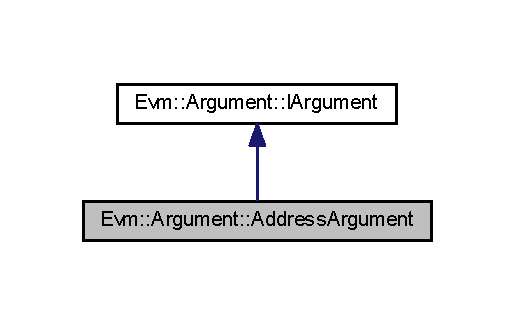
\includegraphics[width=247pt]{struct_evm_1_1_argument_1_1_address_argument__inherit__graph}
\end{center}
\end{figure}


Collaboration diagram for Evm\+:\+:Argument\+:\+:Address\+Argument\+:
\nopagebreak
\begin{figure}[H]
\begin{center}
\leavevmode
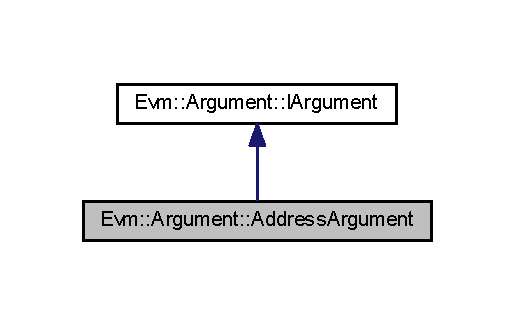
\includegraphics[width=247pt]{struct_evm_1_1_argument_1_1_address_argument__coll__graph}
\end{center}
\end{figure}
\subsection*{Public Member Functions}
\begin{DoxyCompactItemize}
\item 
\mbox{\Hypertarget{struct_evm_1_1_argument_1_1_address_argument_a156c0673b4d0fa8e02bcd5814e24d868}\label{struct_evm_1_1_argument_1_1_address_argument_a156c0673b4d0fa8e02bcd5814e24d868}} 
{\bfseries Address\+Argument} (uint32\+\_\+t value)
\item 
virtual uint64\+\_\+t \mbox{\hyperlink{struct_evm_1_1_argument_1_1_address_argument_a8dfdf1626e06e7c72af39ca3f09ecec7}{get\+Value}} (\mbox{\hyperlink{struct_evm_1_1_thread_context}{Thread\+Context}} \&thread) const override
\begin{DoxyCompactList}\small\item\em Get value. \end{DoxyCompactList}\item 
virtual void \mbox{\hyperlink{struct_evm_1_1_argument_1_1_address_argument_a2fa90885150424134b181ff01704e798}{set\+Value}} (\mbox{\hyperlink{struct_evm_1_1_thread_context}{Thread\+Context}} \&thread, uint64\+\_\+t value) override
\begin{DoxyCompactList}\small\item\em Set value. \end{DoxyCompactList}\item 
virtual string \mbox{\hyperlink{struct_evm_1_1_argument_1_1_address_argument_a4a8ca0f63e6139140f924c2cab9b3d40}{label}} () const override
\begin{DoxyCompactList}\small\item\em Get printable representation of the argument. \end{DoxyCompactList}\item 
virtual string \mbox{\hyperlink{struct_evm_1_1_argument_1_1_address_argument_afaefa598d24c588a0047df1b88033bbd}{print\+Value}} (\mbox{\hyperlink{struct_evm_1_1_thread_context}{Thread\+Context}} \&thread) const override
\begin{DoxyCompactList}\small\item\em Get printable value of the parameter. \end{DoxyCompactList}\end{DoxyCompactItemize}


\subsection{Member Function Documentation}
\mbox{\Hypertarget{struct_evm_1_1_argument_1_1_address_argument_a8dfdf1626e06e7c72af39ca3f09ecec7}\label{struct_evm_1_1_argument_1_1_address_argument_a8dfdf1626e06e7c72af39ca3f09ecec7}} 
\index{Evm\+::\+Argument\+::\+Address\+Argument@{Evm\+::\+Argument\+::\+Address\+Argument}!get\+Value@{get\+Value}}
\index{get\+Value@{get\+Value}!Evm\+::\+Argument\+::\+Address\+Argument@{Evm\+::\+Argument\+::\+Address\+Argument}}
\subsubsection{\texorpdfstring{get\+Value()}{getValue()}}
{\footnotesize\ttfamily uint64\+\_\+t Evm\+::\+Argument\+::\+Address\+Argument\+::get\+Value (\begin{DoxyParamCaption}\item[{\mbox{\hyperlink{struct_evm_1_1_thread_context}{Thread\+Context}} \&}]{thread }\end{DoxyParamCaption}) const\hspace{0.3cm}{\ttfamily [override]}, {\ttfamily [virtual]}}



Get value. 

Return value of the argument 
\begin{DoxyParams}{Parameters}
{\em thread} & Thread context within this argument is used \\
\hline
\end{DoxyParams}
\begin{DoxyReturn}{Returns}
Value of the parameter 
\end{DoxyReturn}


Implements \mbox{\hyperlink{struct_evm_1_1_argument_1_1_i_argument_af01db10f34498344831877847c2fc038}{Evm\+::\+Argument\+::\+I\+Argument}}.

\mbox{\Hypertarget{struct_evm_1_1_argument_1_1_address_argument_a4a8ca0f63e6139140f924c2cab9b3d40}\label{struct_evm_1_1_argument_1_1_address_argument_a4a8ca0f63e6139140f924c2cab9b3d40}} 
\index{Evm\+::\+Argument\+::\+Address\+Argument@{Evm\+::\+Argument\+::\+Address\+Argument}!label@{label}}
\index{label@{label}!Evm\+::\+Argument\+::\+Address\+Argument@{Evm\+::\+Argument\+::\+Address\+Argument}}
\subsubsection{\texorpdfstring{label()}{label()}}
{\footnotesize\ttfamily string Evm\+::\+Argument\+::\+Address\+Argument\+::label (\begin{DoxyParamCaption}{ }\end{DoxyParamCaption}) const\hspace{0.3cm}{\ttfamily [override]}, {\ttfamily [virtual]}}



Get printable representation of the argument. 

\begin{DoxyReturn}{Returns}
string with argument label 
\end{DoxyReturn}


Implements \mbox{\hyperlink{struct_evm_1_1_argument_1_1_i_argument_a35bdae816e89f6f9fc393b6e03c5e521}{Evm\+::\+Argument\+::\+I\+Argument}}.

\mbox{\Hypertarget{struct_evm_1_1_argument_1_1_address_argument_afaefa598d24c588a0047df1b88033bbd}\label{struct_evm_1_1_argument_1_1_address_argument_afaefa598d24c588a0047df1b88033bbd}} 
\index{Evm\+::\+Argument\+::\+Address\+Argument@{Evm\+::\+Argument\+::\+Address\+Argument}!print\+Value@{print\+Value}}
\index{print\+Value@{print\+Value}!Evm\+::\+Argument\+::\+Address\+Argument@{Evm\+::\+Argument\+::\+Address\+Argument}}
\subsubsection{\texorpdfstring{print\+Value()}{printValue()}}
{\footnotesize\ttfamily string Evm\+::\+Argument\+::\+Address\+Argument\+::print\+Value (\begin{DoxyParamCaption}\item[{\mbox{\hyperlink{struct_evm_1_1_thread_context}{Thread\+Context}} \&}]{thread }\end{DoxyParamCaption}) const\hspace{0.3cm}{\ttfamily [override]}, {\ttfamily [virtual]}}



Get printable value of the parameter. 


\begin{DoxyParams}{Parameters}
{\em thread} & Thread context within this argument is used \\
\hline
\end{DoxyParams}
\begin{DoxyReturn}{Returns}
string with argument value 
\end{DoxyReturn}


Implements \mbox{\hyperlink{struct_evm_1_1_argument_1_1_i_argument_afcab2d2a1515518a111881a635c83da3}{Evm\+::\+Argument\+::\+I\+Argument}}.

\mbox{\Hypertarget{struct_evm_1_1_argument_1_1_address_argument_a2fa90885150424134b181ff01704e798}\label{struct_evm_1_1_argument_1_1_address_argument_a2fa90885150424134b181ff01704e798}} 
\index{Evm\+::\+Argument\+::\+Address\+Argument@{Evm\+::\+Argument\+::\+Address\+Argument}!set\+Value@{set\+Value}}
\index{set\+Value@{set\+Value}!Evm\+::\+Argument\+::\+Address\+Argument@{Evm\+::\+Argument\+::\+Address\+Argument}}
\subsubsection{\texorpdfstring{set\+Value()}{setValue()}}
{\footnotesize\ttfamily void Evm\+::\+Argument\+::\+Address\+Argument\+::set\+Value (\begin{DoxyParamCaption}\item[{\mbox{\hyperlink{struct_evm_1_1_thread_context}{Thread\+Context}} \&}]{thread,  }\item[{uint64\+\_\+t}]{value }\end{DoxyParamCaption})\hspace{0.3cm}{\ttfamily [override]}, {\ttfamily [virtual]}}



Set value. 

Set value of the argument. \begin{DoxyWarning}{Warning}
For read-\/only arguments this throws an exception 
\end{DoxyWarning}

\begin{DoxyParams}{Parameters}
{\em thread} & Thread context within this argument is used \\
\hline
{\em value} & New value of the parameter \\
\hline
\end{DoxyParams}


Implements \mbox{\hyperlink{struct_evm_1_1_argument_1_1_i_argument_a24e4c76f2750e664e3895d2ff4b9146d}{Evm\+::\+Argument\+::\+I\+Argument}}.



The documentation for this struct was generated from the following files\+:\begin{DoxyCompactItemize}
\item 
Evm/\mbox{\hyperlink{_argument_8h}{Argument.\+h}}\item 
Evm/Argument.\+cpp\end{DoxyCompactItemize}

\hypertarget{struct_evm_1_1_operation_1_1_address_operation_factory}{}\section{Evm\+:\+:Operation\+:\+:Address\+Operation\+Factory$<$ T $>$ Struct Template Reference}
\label{struct_evm_1_1_operation_1_1_address_operation_factory}\index{Evm\+::\+Operation\+::\+Address\+Operation\+Factory$<$ T $>$@{Evm\+::\+Operation\+::\+Address\+Operation\+Factory$<$ T $>$}}


Inheritance diagram for Evm\+:\+:Operation\+:\+:Address\+Operation\+Factory$<$ T $>$\+:
\nopagebreak
\begin{figure}[H]
\begin{center}
\leavevmode
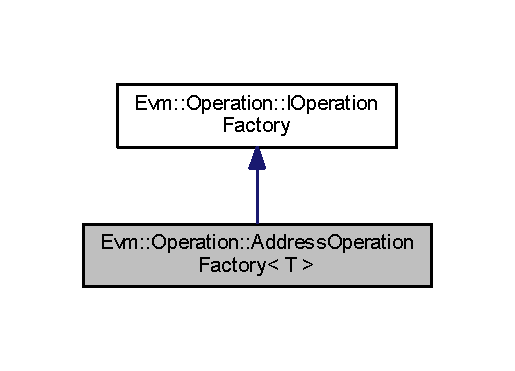
\includegraphics[width=247pt]{struct_evm_1_1_operation_1_1_address_operation_factory__inherit__graph}
\end{center}
\end{figure}


Collaboration diagram for Evm\+:\+:Operation\+:\+:Address\+Operation\+Factory$<$ T $>$\+:
\nopagebreak
\begin{figure}[H]
\begin{center}
\leavevmode
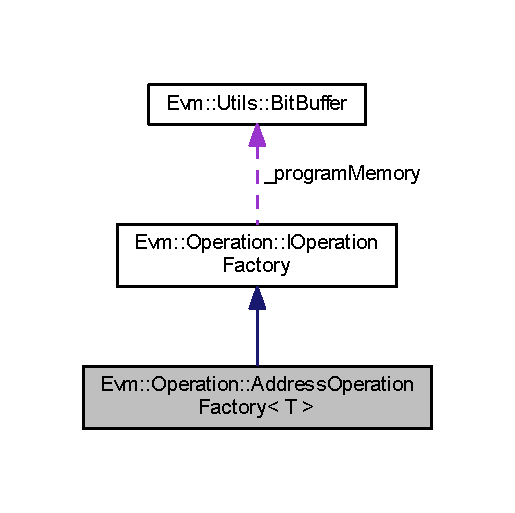
\includegraphics[width=247pt]{struct_evm_1_1_operation_1_1_address_operation_factory__coll__graph}
\end{center}
\end{figure}
\subsection*{Public Member Functions}
\begin{DoxyCompactItemize}
\item 
\mbox{\Hypertarget{struct_evm_1_1_operation_1_1_address_operation_factory_a1f8ebaf24e08497ded428cf93ddac1d6}\label{struct_evm_1_1_operation_1_1_address_operation_factory_a1f8ebaf24e08497ded428cf93ddac1d6}} 
virtual Operation\+Ptr {\bfseries build} (uint32\+\_\+t \&offset)
\item 
\mbox{\Hypertarget{struct_evm_1_1_operation_1_1_address_operation_factory_a7621b51ca2bc125b36be673486e33781}\label{struct_evm_1_1_operation_1_1_address_operation_factory_a7621b51ca2bc125b36be673486e33781}} 
{\bfseries I\+Operation\+Factory} (const string \&opcode, const \mbox{\hyperlink{struct_evm_1_1_utils_1_1_bit_buffer}{Utils\+::\+Bit\+Buffer}} \&program\+Memory)
\end{DoxyCompactItemize}
\subsection*{Additional Inherited Members}


The documentation for this struct was generated from the following file\+:\begin{DoxyCompactItemize}
\item 
Evm/Operation\+Factory.\+h\end{DoxyCompactItemize}

\hypertarget{struct_evm_1_1_application}{}\section{Evm\+:\+:Application Struct Reference}
\label{struct_evm_1_1_application}\index{Evm\+::\+Application@{Evm\+::\+Application}}


Main E\+VM application class.  




{\ttfamily \#include $<$Application.\+h$>$}

\subsection*{Public Types}
\begin{DoxyCompactItemize}
\item 
\mbox{\Hypertarget{struct_evm_1_1_application_aadbcc3dd7f4464ecb028bc5692cde348}\label{struct_evm_1_1_application_aadbcc3dd7f4464ecb028bc5692cde348}} 
using {\bfseries Thread\+Contex\+Ptr} = unique\+\_\+ptr$<$ \mbox{\hyperlink{struct_evm_1_1_thread_context}{Thread\+Context}} $>$
\item 
\mbox{\Hypertarget{struct_evm_1_1_application_ad36d3ad5af0c655ce793abe07a241e5d}\label{struct_evm_1_1_application_ad36d3ad5af0c655ce793abe07a241e5d}} 
using {\bfseries Thread\+List} = vector$<$ Thread\+Contex\+Ptr $>$
\item 
\mbox{\Hypertarget{struct_evm_1_1_application_acf0318d8baa36b9ea02f89c6f2d99874}\label{struct_evm_1_1_application_acf0318d8baa36b9ea02f89c6f2d99874}} 
using {\bfseries Lock\+List} = map$<$ uint64\+\_\+t, mutex $>$
\end{DoxyCompactItemize}
\subsection*{Public Member Functions}
\begin{DoxyCompactItemize}
\item 
\mbox{\hyperlink{struct_evm_1_1_application_ac0dcf0cf2c0b1b3e70024a07536534a2}{Application}} (\mbox{\hyperlink{struct_evm_1_1_cli_configuration}{Cli\+Configuration}} \&config)
\begin{DoxyCompactList}\small\item\em Constructor. \end{DoxyCompactList}\item 
\mbox{\Hypertarget{struct_evm_1_1_application_ab209f49ad8c73c1f3fde7c66585284fb}\label{struct_evm_1_1_application_ab209f49ad8c73c1f3fde7c66585284fb}} 
\mbox{\hyperlink{struct_evm_1_1_application_ab209f49ad8c73c1f3fde7c66585284fb}{$\sim$\+Application}} ()
\begin{DoxyCompactList}\small\item\em Destructor. \end{DoxyCompactList}\item 
void \mbox{\hyperlink{struct_evm_1_1_application_a26403ae00f2a6d2ef5fa3e78e183f4ce}{run}} ()
\begin{DoxyCompactList}\small\item\em Run the evm execution. \end{DoxyCompactList}\item 
void \mbox{\hyperlink{struct_evm_1_1_application_a17e8baa475b18f35f70823a91f12304c}{wait}} ()
\begin{DoxyCompactList}\small\item\em Wait for execution. \end{DoxyCompactList}\item 
uint64\+\_\+t \mbox{\hyperlink{struct_evm_1_1_application_a4b5883ca11f132aa33ede5a2acd997cc}{run\+New\+Thread}} (\mbox{\hyperlink{struct_evm_1_1_thread_context}{Thread\+Context}} \&caller, uint32\+\_\+t address)
\begin{DoxyCompactList}\small\item\em Spawn new evm thread. \end{DoxyCompactList}\item 
void \mbox{\hyperlink{struct_evm_1_1_application_a71ad6065512bd28e0208fee37597484b}{join\+Thread}} (uint64\+\_\+t thread\+Id)
\begin{DoxyCompactList}\small\item\em Join a thread. \end{DoxyCompactList}\item 
void \mbox{\hyperlink{struct_evm_1_1_application_a102467a47420ec04d5ab1e68bd465579}{lock}} (uint64\+\_\+t lock\+ID)
\begin{DoxyCompactList}\small\item\em Obtain a lock. \end{DoxyCompactList}\item 
void \mbox{\hyperlink{struct_evm_1_1_application_a1f1efb23d8d815d3b92b9a2f85b328f1}{unlock}} (uint64\+\_\+t lock\+ID)
\begin{DoxyCompactList}\small\item\em Release a lock. \end{DoxyCompactList}\item 
\mbox{\hyperlink{struct_evm_1_1_utils_1_1_memory}{Utils\+::\+Memory}} \& \mbox{\hyperlink{struct_evm_1_1_application_ae298c9f84fb6a0a4d51aa6ca39dce96a}{data\+Memory}} ()
\begin{DoxyCompactList}\small\item\em Get reference to data memory. \end{DoxyCompactList}\item 
const \mbox{\hyperlink{struct_evm_1_1_utils_1_1_bit_buffer}{Utils\+::\+Bit\+Buffer}} \& \mbox{\hyperlink{struct_evm_1_1_application_a0e55226ef456356c5d25f8da1c9ae926}{program\+Memory}} () const
\begin{DoxyCompactList}\small\item\em Get reference to program memory. \end{DoxyCompactList}\item 
fstream \& \mbox{\hyperlink{struct_evm_1_1_application_a9cb5d822b96435dd1e48f02e3a14e66a}{input\+File}} ()
\begin{DoxyCompactList}\small\item\em Get reference to input file. \end{DoxyCompactList}\item 
const string \& \mbox{\hyperlink{struct_evm_1_1_application_ac7916137b6e8cb5ae323e1ec9ce9f050}{input\+File\+Name}} () const
\begin{DoxyCompactList}\small\item\em Get input file name. \end{DoxyCompactList}\item 
\mbox{\Hypertarget{struct_evm_1_1_application_a4baabf3c0d1eeef319952726eed7f8a1}\label{struct_evm_1_1_application_a4baabf3c0d1eeef319952726eed7f8a1}} 
const \mbox{\hyperlink{struct_evm_1_1_cli_configuration}{Cli\+Configuration}} \& {\bfseries configuartion} () const
\item 
\mbox{\Hypertarget{struct_evm_1_1_application_a0ccd71f9edb98d0255597973a1105d08}\label{struct_evm_1_1_application_a0ccd71f9edb98d0255597973a1105d08}} 
{\bfseries Application} (const \mbox{\hyperlink{struct_evm_1_1_application}{Application}} \&)=delete
\item 
\mbox{\Hypertarget{struct_evm_1_1_application_ad280fab63abb3218d0f7619d4c31359a}\label{struct_evm_1_1_application_ad280fab63abb3218d0f7619d4c31359a}} 
{\bfseries Application} (\mbox{\hyperlink{struct_evm_1_1_application}{Application}} \&\&)=delete
\item 
\mbox{\Hypertarget{struct_evm_1_1_application_a5dc9e3d6c4bddc6d0339d3d12b9a48d8}\label{struct_evm_1_1_application_a5dc9e3d6c4bddc6d0339d3d12b9a48d8}} 
\mbox{\hyperlink{struct_evm_1_1_application}{Application}} \& {\bfseries operator=} (const \mbox{\hyperlink{struct_evm_1_1_application}{Application}} \&)=delete
\item 
\mbox{\Hypertarget{struct_evm_1_1_application_a93122a21cf168f84d6ca24f7db680589}\label{struct_evm_1_1_application_a93122a21cf168f84d6ca24f7db680589}} 
\mbox{\hyperlink{struct_evm_1_1_application}{Application}} \& {\bfseries operator=} (\mbox{\hyperlink{struct_evm_1_1_application}{Application}} \&\&)=delete
\end{DoxyCompactItemize}


\subsection{Detailed Description}
Main E\+VM application class. 

The class is responsible for parsing and execution of E\+VM files. It is responsible for parsing and running evm file. It also provides data and program memories, thread list, locks list input file as well as interfaces to these objects. 

\subsection{Constructor \& Destructor Documentation}
\mbox{\Hypertarget{struct_evm_1_1_application_ac0dcf0cf2c0b1b3e70024a07536534a2}\label{struct_evm_1_1_application_ac0dcf0cf2c0b1b3e70024a07536534a2}} 
\index{Evm\+::\+Application@{Evm\+::\+Application}!Application@{Application}}
\index{Application@{Application}!Evm\+::\+Application@{Evm\+::\+Application}}
\subsubsection{\texorpdfstring{Application()}{Application()}}
{\footnotesize\ttfamily Evm\+::\+Application\+::\+Application (\begin{DoxyParamCaption}\item[{\mbox{\hyperlink{struct_evm_1_1_cli_configuration}{Cli\+Configuration}} \&}]{config }\end{DoxyParamCaption})}



Constructor. 

The constructor is initializes thread list, lock list and other internal structures. It also parses an evm file, validate it, and initializes data and program memories. 
\begin{DoxyParams}{Parameters}
{\em config} & reference to configuration file \\
\hline
\end{DoxyParams}

\begin{DoxyExceptions}{Exceptions}
{\em \mbox{\hyperlink{struct_evm_1_1_runtime_error}{Runtime\+Error}}} & \\
\hline
\end{DoxyExceptions}


\subsection{Member Function Documentation}
\mbox{\Hypertarget{struct_evm_1_1_application_ae298c9f84fb6a0a4d51aa6ca39dce96a}\label{struct_evm_1_1_application_ae298c9f84fb6a0a4d51aa6ca39dce96a}} 
\index{Evm\+::\+Application@{Evm\+::\+Application}!data\+Memory@{data\+Memory}}
\index{data\+Memory@{data\+Memory}!Evm\+::\+Application@{Evm\+::\+Application}}
\subsubsection{\texorpdfstring{data\+Memory()}{dataMemory()}}
{\footnotesize\ttfamily \mbox{\hyperlink{struct_evm_1_1_utils_1_1_memory}{Utils\+::\+Memory}} \& Evm\+::\+Application\+::data\+Memory (\begin{DoxyParamCaption}{ }\end{DoxyParamCaption})}



Get reference to data memory. 

A\+PI function for evm library. Getter of data memory. \begin{DoxyReturn}{Returns}
reference to data memory object 
\end{DoxyReturn}
\mbox{\Hypertarget{struct_evm_1_1_application_a9cb5d822b96435dd1e48f02e3a14e66a}\label{struct_evm_1_1_application_a9cb5d822b96435dd1e48f02e3a14e66a}} 
\index{Evm\+::\+Application@{Evm\+::\+Application}!input\+File@{input\+File}}
\index{input\+File@{input\+File}!Evm\+::\+Application@{Evm\+::\+Application}}
\subsubsection{\texorpdfstring{input\+File()}{inputFile()}}
{\footnotesize\ttfamily fstream \& Evm\+::\+Application\+::input\+File (\begin{DoxyParamCaption}{ }\end{DoxyParamCaption})}



Get reference to input file. 

The function returns reference to inpute file, but only if the file is given. If the file is not given be an user the function throws \mbox{\hyperlink{struct_evm_1_1_input_file_runtime_error}{Input\+File\+Runtime\+Error}} exception \begin{DoxyReturn}{Returns}
reference to input file 
\end{DoxyReturn}

\begin{DoxyExceptions}{Exceptions}
{\em \mbox{\hyperlink{struct_evm_1_1_runtime_error}{Runtime\+Error}}} & \\
\hline
\end{DoxyExceptions}
\mbox{\Hypertarget{struct_evm_1_1_application_ac7916137b6e8cb5ae323e1ec9ce9f050}\label{struct_evm_1_1_application_ac7916137b6e8cb5ae323e1ec9ce9f050}} 
\index{Evm\+::\+Application@{Evm\+::\+Application}!input\+File\+Name@{input\+File\+Name}}
\index{input\+File\+Name@{input\+File\+Name}!Evm\+::\+Application@{Evm\+::\+Application}}
\subsubsection{\texorpdfstring{input\+File\+Name()}{inputFileName()}}
{\footnotesize\ttfamily const string \& Evm\+::\+Application\+::input\+File\+Name (\begin{DoxyParamCaption}{ }\end{DoxyParamCaption}) const}



Get input file name. 

The function returns input file name \begin{DoxyReturn}{Returns}
input file name 
\end{DoxyReturn}
\mbox{\Hypertarget{struct_evm_1_1_application_a71ad6065512bd28e0208fee37597484b}\label{struct_evm_1_1_application_a71ad6065512bd28e0208fee37597484b}} 
\index{Evm\+::\+Application@{Evm\+::\+Application}!join\+Thread@{join\+Thread}}
\index{join\+Thread@{join\+Thread}!Evm\+::\+Application@{Evm\+::\+Application}}
\subsubsection{\texorpdfstring{join\+Thread()}{joinThread()}}
{\footnotesize\ttfamily void Evm\+::\+Application\+::join\+Thread (\begin{DoxyParamCaption}\item[{uint64\+\_\+t}]{thread\+Id }\end{DoxyParamCaption})}



Join a thread. 

A\+PI function for evm library. Suspend current thread execution until a thread with given ID is done \begin{DoxyNote}{Note}
This is blocking function 
\end{DoxyNote}

\begin{DoxyParams}{Parameters}
{\em thread\+Id} & id of a related thread \\
\hline
\end{DoxyParams}

\begin{DoxyExceptions}{Exceptions}
{\em \mbox{\hyperlink{struct_evm_1_1_runtime_error}{Runtime\+Error}}} & \\
\hline
\end{DoxyExceptions}
\mbox{\Hypertarget{struct_evm_1_1_application_a102467a47420ec04d5ab1e68bd465579}\label{struct_evm_1_1_application_a102467a47420ec04d5ab1e68bd465579}} 
\index{Evm\+::\+Application@{Evm\+::\+Application}!lock@{lock}}
\index{lock@{lock}!Evm\+::\+Application@{Evm\+::\+Application}}
\subsubsection{\texorpdfstring{lock()}{lock()}}
{\footnotesize\ttfamily void Evm\+::\+Application\+::lock (\begin{DoxyParamCaption}\item[{uint64\+\_\+t}]{lock\+ID }\end{DoxyParamCaption})}



Obtain a lock. 

A\+PI function for evm library. Obtain a lock with given ID. When the lock doesn\textquotesingle{}t exist it will be created. If the lock is already obtained, the thread will be suspended. \begin{DoxyNote}{Note}
The function is blocking when the lock is already obtained~\newline
otherwise is is non-\/blocking 
\end{DoxyNote}

\begin{DoxyParams}{Parameters}
{\em lock\+ID} & ID of the lock \\
\hline
\end{DoxyParams}

\begin{DoxyExceptions}{Exceptions}
{\em \mbox{\hyperlink{struct_evm_1_1_runtime_error}{Runtime\+Error}}} & \\
\hline
\end{DoxyExceptions}
\mbox{\Hypertarget{struct_evm_1_1_application_a0e55226ef456356c5d25f8da1c9ae926}\label{struct_evm_1_1_application_a0e55226ef456356c5d25f8da1c9ae926}} 
\index{Evm\+::\+Application@{Evm\+::\+Application}!program\+Memory@{program\+Memory}}
\index{program\+Memory@{program\+Memory}!Evm\+::\+Application@{Evm\+::\+Application}}
\subsubsection{\texorpdfstring{program\+Memory()}{programMemory()}}
{\footnotesize\ttfamily const \mbox{\hyperlink{struct_evm_1_1_utils_1_1_bit_buffer}{Utils\+::\+Bit\+Buffer}} \& Evm\+::\+Application\+::program\+Memory (\begin{DoxyParamCaption}{ }\end{DoxyParamCaption}) const}



Get reference to program memory. 

A\+PI function for evm library. Getter of program memory. Program memory is bit accessed. Due to thread safety, it is read only memory. \begin{DoxyReturn}{Returns}
reference to program memory 
\end{DoxyReturn}
\mbox{\Hypertarget{struct_evm_1_1_application_a26403ae00f2a6d2ef5fa3e78e183f4ce}\label{struct_evm_1_1_application_a26403ae00f2a6d2ef5fa3e78e183f4ce}} 
\index{Evm\+::\+Application@{Evm\+::\+Application}!run@{run}}
\index{run@{run}!Evm\+::\+Application@{Evm\+::\+Application}}
\subsubsection{\texorpdfstring{run()}{run()}}
{\footnotesize\ttfamily void Evm\+::\+Application\+::run (\begin{DoxyParamCaption}{ }\end{DoxyParamCaption})}



Run the evm execution. 

Running the evm file execution. It creates at least one thread. \begin{DoxyNote}{Note}
This is non-\/blocking function 
\end{DoxyNote}

\begin{DoxyExceptions}{Exceptions}
{\em \mbox{\hyperlink{struct_evm_1_1_runtime_error}{Runtime\+Error}}} & \\
\hline
\end{DoxyExceptions}
\mbox{\Hypertarget{struct_evm_1_1_application_a4b5883ca11f132aa33ede5a2acd997cc}\label{struct_evm_1_1_application_a4b5883ca11f132aa33ede5a2acd997cc}} 
\index{Evm\+::\+Application@{Evm\+::\+Application}!run\+New\+Thread@{run\+New\+Thread}}
\index{run\+New\+Thread@{run\+New\+Thread}!Evm\+::\+Application@{Evm\+::\+Application}}
\subsubsection{\texorpdfstring{run\+New\+Thread()}{runNewThread()}}
{\footnotesize\ttfamily uint64\+\_\+t Evm\+::\+Application\+::run\+New\+Thread (\begin{DoxyParamCaption}\item[{\mbox{\hyperlink{struct_evm_1_1_thread_context}{Thread\+Context}} \&}]{caller,  }\item[{uint32\+\_\+t}]{address }\end{DoxyParamCaption})}



Spawn new evm thread. 

A\+PI function for evm library. The function creates new evm thread based on caller. The new thread\textquotesingle{}s program counter is set to address value. \begin{DoxyNote}{Note}
This is non-\/blocking function 
\end{DoxyNote}

\begin{DoxyParams}{Parameters}
{\em caller} & reference to caller thread \\
\hline
{\em address} & initial value to the new thread program counter \\
\hline
\end{DoxyParams}
\begin{DoxyReturn}{Returns}
new thread ID 
\end{DoxyReturn}

\begin{DoxyExceptions}{Exceptions}
{\em \mbox{\hyperlink{struct_evm_1_1_runtime_error}{Runtime\+Error}}} & \\
\hline
\end{DoxyExceptions}
\mbox{\Hypertarget{struct_evm_1_1_application_a1f1efb23d8d815d3b92b9a2f85b328f1}\label{struct_evm_1_1_application_a1f1efb23d8d815d3b92b9a2f85b328f1}} 
\index{Evm\+::\+Application@{Evm\+::\+Application}!unlock@{unlock}}
\index{unlock@{unlock}!Evm\+::\+Application@{Evm\+::\+Application}}
\subsubsection{\texorpdfstring{unlock()}{unlock()}}
{\footnotesize\ttfamily void Evm\+::\+Application\+::unlock (\begin{DoxyParamCaption}\item[{uint64\+\_\+t}]{lock\+ID }\end{DoxyParamCaption})}



Release a lock. 

A\+PI function for evm library. Release a lock with given ID. When the lock doesn\textquotesingle{}t exist \mbox{\hyperlink{struct_evm_1_1_bad_lock_i_d_runtime_error}{Bad\+Lock\+I\+D\+Runtime\+Error}} exception will be thrown \begin{DoxyNote}{Note}
This is non-\/blocking function 
\end{DoxyNote}

\begin{DoxyParams}{Parameters}
{\em lock\+ID} & ID of the lock \\
\hline
\end{DoxyParams}

\begin{DoxyExceptions}{Exceptions}
{\em \mbox{\hyperlink{struct_evm_1_1_runtime_error}{Runtime\+Error}}} & \\
\hline
\end{DoxyExceptions}
\mbox{\Hypertarget{struct_evm_1_1_application_a17e8baa475b18f35f70823a91f12304c}\label{struct_evm_1_1_application_a17e8baa475b18f35f70823a91f12304c}} 
\index{Evm\+::\+Application@{Evm\+::\+Application}!wait@{wait}}
\index{wait@{wait}!Evm\+::\+Application@{Evm\+::\+Application}}
\subsubsection{\texorpdfstring{wait()}{wait()}}
{\footnotesize\ttfamily void Evm\+::\+Application\+::wait (\begin{DoxyParamCaption}{ }\end{DoxyParamCaption})}



Wait for execution. 

The function waits until the main evm thread is done. If the main thread is done, other threads are terminated and joined. \begin{DoxyNote}{Note}
This is blocking function 
\end{DoxyNote}

\begin{DoxyExceptions}{Exceptions}
{\em \mbox{\hyperlink{struct_evm_1_1_runtime_error}{Runtime\+Error}}} & \\
\hline
\end{DoxyExceptions}


The documentation for this struct was generated from the following files\+:\begin{DoxyCompactItemize}
\item 
Evm/\mbox{\hyperlink{_application_8h}{Application.\+h}}\item 
Evm/\mbox{\hyperlink{_application_8cpp}{Application.\+cpp}}\end{DoxyCompactItemize}

\hypertarget{struct_evm_1_1_operation_1_1_arg1_arg2_arg3_arg4_operation_factory}{}\section{Evm\+:\+:Operation\+:\+:Arg1\+Arg2\+Arg3\+Arg4\+Operation\+Factory$<$ T $>$ Struct Template Reference}
\label{struct_evm_1_1_operation_1_1_arg1_arg2_arg3_arg4_operation_factory}\index{Evm\+::\+Operation\+::\+Arg1\+Arg2\+Arg3\+Arg4\+Operation\+Factory$<$ T $>$@{Evm\+::\+Operation\+::\+Arg1\+Arg2\+Arg3\+Arg4\+Operation\+Factory$<$ T $>$}}


Inheritance diagram for Evm\+:\+:Operation\+:\+:Arg1\+Arg2\+Arg3\+Arg4\+Operation\+Factory$<$ T $>$\+:
\nopagebreak
\begin{figure}[H]
\begin{center}
\leavevmode
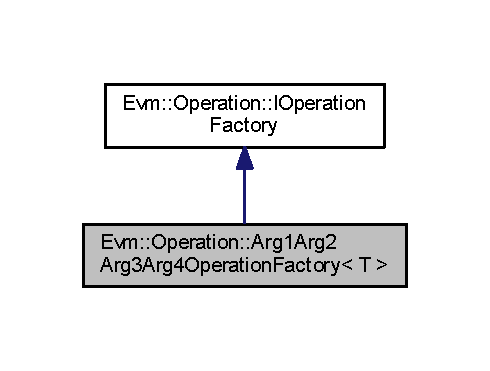
\includegraphics[width=235pt]{struct_evm_1_1_operation_1_1_arg1_arg2_arg3_arg4_operation_factory__inherit__graph}
\end{center}
\end{figure}


Collaboration diagram for Evm\+:\+:Operation\+:\+:Arg1\+Arg2\+Arg3\+Arg4\+Operation\+Factory$<$ T $>$\+:
\nopagebreak
\begin{figure}[H]
\begin{center}
\leavevmode
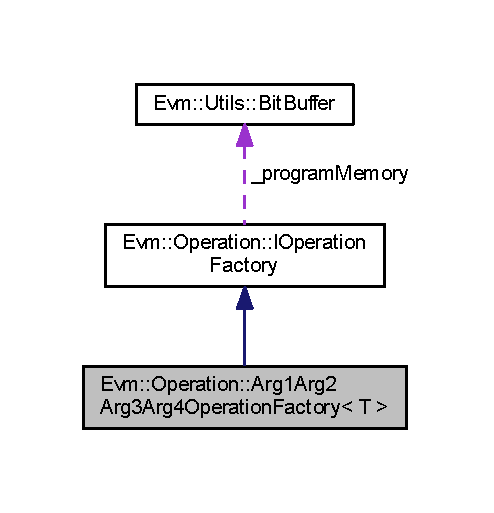
\includegraphics[width=237pt]{struct_evm_1_1_operation_1_1_arg1_arg2_arg3_arg4_operation_factory__coll__graph}
\end{center}
\end{figure}
\subsection*{Public Member Functions}
\begin{DoxyCompactItemize}
\item 
\mbox{\Hypertarget{struct_evm_1_1_operation_1_1_arg1_arg2_arg3_arg4_operation_factory_a376b731a1310d37539dbbe85e37cb53b}\label{struct_evm_1_1_operation_1_1_arg1_arg2_arg3_arg4_operation_factory_a376b731a1310d37539dbbe85e37cb53b}} 
virtual Operation\+Ptr {\bfseries build} (uint32\+\_\+t \&offset)
\item 
\mbox{\Hypertarget{struct_evm_1_1_operation_1_1_arg1_arg2_arg3_arg4_operation_factory_a7621b51ca2bc125b36be673486e33781}\label{struct_evm_1_1_operation_1_1_arg1_arg2_arg3_arg4_operation_factory_a7621b51ca2bc125b36be673486e33781}} 
{\bfseries I\+Operation\+Factory} (const string \&opcode, const \mbox{\hyperlink{struct_evm_1_1_utils_1_1_bit_buffer}{Utils\+::\+Bit\+Buffer}} \&program\+Memory)
\end{DoxyCompactItemize}
\subsection*{Additional Inherited Members}


The documentation for this struct was generated from the following file\+:\begin{DoxyCompactItemize}
\item 
Evm/Operation\+Factory.\+h\end{DoxyCompactItemize}

\hypertarget{struct_evm_1_1_operation_1_1_arg1_arg2_arg3_operation_factory}{}\section{Evm\+:\+:Operation\+:\+:Arg1\+Arg2\+Arg3\+Operation\+Factory$<$ T $>$ Struct Template Reference}
\label{struct_evm_1_1_operation_1_1_arg1_arg2_arg3_operation_factory}\index{Evm\+::\+Operation\+::\+Arg1\+Arg2\+Arg3\+Operation\+Factory$<$ T $>$@{Evm\+::\+Operation\+::\+Arg1\+Arg2\+Arg3\+Operation\+Factory$<$ T $>$}}


Inheritance diagram for Evm\+:\+:Operation\+:\+:Arg1\+Arg2\+Arg3\+Operation\+Factory$<$ T $>$\+:
\nopagebreak
\begin{figure}[H]
\begin{center}
\leavevmode
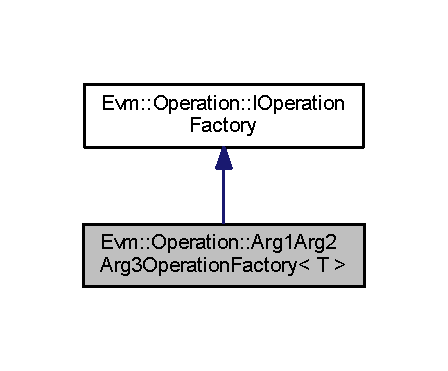
\includegraphics[width=215pt]{struct_evm_1_1_operation_1_1_arg1_arg2_arg3_operation_factory__inherit__graph}
\end{center}
\end{figure}


Collaboration diagram for Evm\+:\+:Operation\+:\+:Arg1\+Arg2\+Arg3\+Operation\+Factory$<$ T $>$\+:
\nopagebreak
\begin{figure}[H]
\begin{center}
\leavevmode
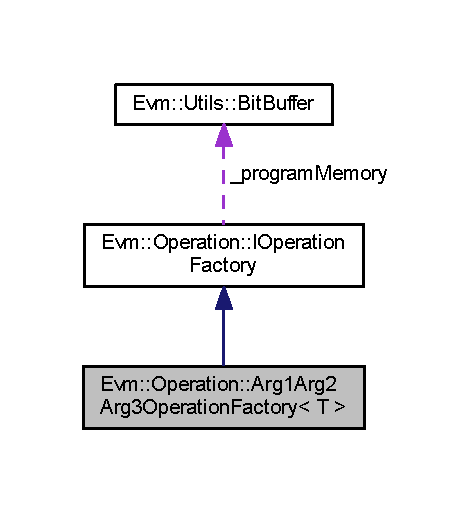
\includegraphics[width=227pt]{struct_evm_1_1_operation_1_1_arg1_arg2_arg3_operation_factory__coll__graph}
\end{center}
\end{figure}
\subsection*{Public Member Functions}
\begin{DoxyCompactItemize}
\item 
\mbox{\Hypertarget{struct_evm_1_1_operation_1_1_arg1_arg2_arg3_operation_factory_a4d82b51c90435be3ef7c9e6df8d721b1}\label{struct_evm_1_1_operation_1_1_arg1_arg2_arg3_operation_factory_a4d82b51c90435be3ef7c9e6df8d721b1}} 
virtual Operation\+Ptr {\bfseries build} (uint32\+\_\+t \&offset)
\item 
\mbox{\Hypertarget{struct_evm_1_1_operation_1_1_arg1_arg2_arg3_operation_factory_a7621b51ca2bc125b36be673486e33781}\label{struct_evm_1_1_operation_1_1_arg1_arg2_arg3_operation_factory_a7621b51ca2bc125b36be673486e33781}} 
{\bfseries I\+Operation\+Factory} (const string \&opcode, const \mbox{\hyperlink{struct_evm_1_1_utils_1_1_bit_buffer}{Utils\+::\+Bit\+Buffer}} \&program\+Memory)
\end{DoxyCompactItemize}
\subsection*{Additional Inherited Members}


The documentation for this struct was generated from the following file\+:\begin{DoxyCompactItemize}
\item 
Evm/Operation\+Factory.\+h\end{DoxyCompactItemize}

\hypertarget{struct_evm_1_1_operation_1_1_arg1_arg2_operation_factory}{}\section{Evm\+:\+:Operation\+:\+:Arg1\+Arg2\+Operation\+Factory$<$ T $>$ Struct Template Reference}
\label{struct_evm_1_1_operation_1_1_arg1_arg2_operation_factory}\index{Evm\+::\+Operation\+::\+Arg1\+Arg2\+Operation\+Factory$<$ T $>$@{Evm\+::\+Operation\+::\+Arg1\+Arg2\+Operation\+Factory$<$ T $>$}}


Inheritance diagram for Evm\+:\+:Operation\+:\+:Arg1\+Arg2\+Operation\+Factory$<$ T $>$\+:
\nopagebreak
\begin{figure}[H]
\begin{center}
\leavevmode
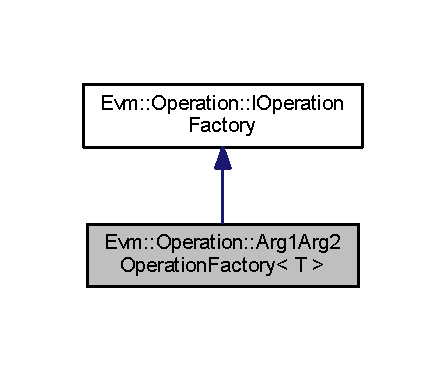
\includegraphics[width=214pt]{struct_evm_1_1_operation_1_1_arg1_arg2_operation_factory__inherit__graph}
\end{center}
\end{figure}


Collaboration diagram for Evm\+:\+:Operation\+:\+:Arg1\+Arg2\+Operation\+Factory$<$ T $>$\+:
\nopagebreak
\begin{figure}[H]
\begin{center}
\leavevmode
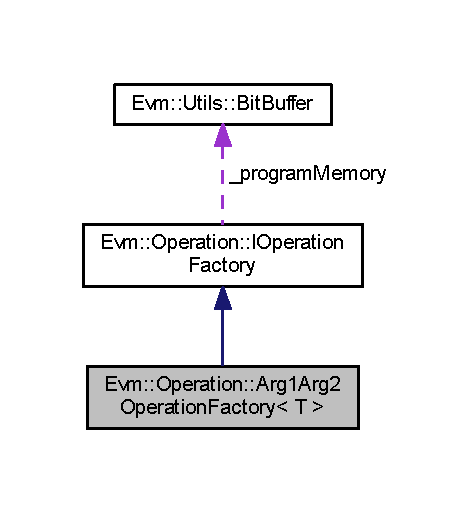
\includegraphics[width=226pt]{struct_evm_1_1_operation_1_1_arg1_arg2_operation_factory__coll__graph}
\end{center}
\end{figure}
\subsection*{Public Member Functions}
\begin{DoxyCompactItemize}
\item 
\mbox{\Hypertarget{struct_evm_1_1_operation_1_1_arg1_arg2_operation_factory_a7c976bc175cab199e6f2378e5025b541}\label{struct_evm_1_1_operation_1_1_arg1_arg2_operation_factory_a7c976bc175cab199e6f2378e5025b541}} 
virtual Operation\+Ptr {\bfseries build} (uint32\+\_\+t \&offset)
\item 
\mbox{\Hypertarget{struct_evm_1_1_operation_1_1_arg1_arg2_operation_factory_a7621b51ca2bc125b36be673486e33781}\label{struct_evm_1_1_operation_1_1_arg1_arg2_operation_factory_a7621b51ca2bc125b36be673486e33781}} 
{\bfseries I\+Operation\+Factory} (const string \&opcode, const \mbox{\hyperlink{struct_evm_1_1_utils_1_1_bit_buffer}{Utils\+::\+Bit\+Buffer}} \&program\+Memory)
\end{DoxyCompactItemize}
\subsection*{Additional Inherited Members}


The documentation for this struct was generated from the following file\+:\begin{DoxyCompactItemize}
\item 
Evm/Operation\+Factory.\+h\end{DoxyCompactItemize}

\hypertarget{struct_evm_1_1_operation_1_1_arg1_operation_factory}{}\section{Evm\+:\+:Operation\+:\+:Arg1\+Operation\+Factory$<$ T $>$ Struct Template Reference}
\label{struct_evm_1_1_operation_1_1_arg1_operation_factory}\index{Evm\+::\+Operation\+::\+Arg1\+Operation\+Factory$<$ T $>$@{Evm\+::\+Operation\+::\+Arg1\+Operation\+Factory$<$ T $>$}}


Inheritance diagram for Evm\+:\+:Operation\+:\+:Arg1\+Operation\+Factory$<$ T $>$\+:
\nopagebreak
\begin{figure}[H]
\begin{center}
\leavevmode
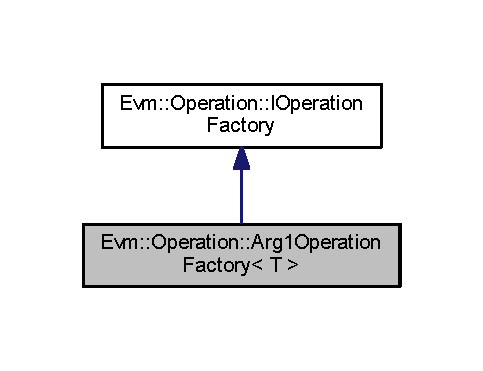
\includegraphics[width=232pt]{struct_evm_1_1_operation_1_1_arg1_operation_factory__inherit__graph}
\end{center}
\end{figure}


Collaboration diagram for Evm\+:\+:Operation\+:\+:Arg1\+Operation\+Factory$<$ T $>$\+:
\nopagebreak
\begin{figure}[H]
\begin{center}
\leavevmode
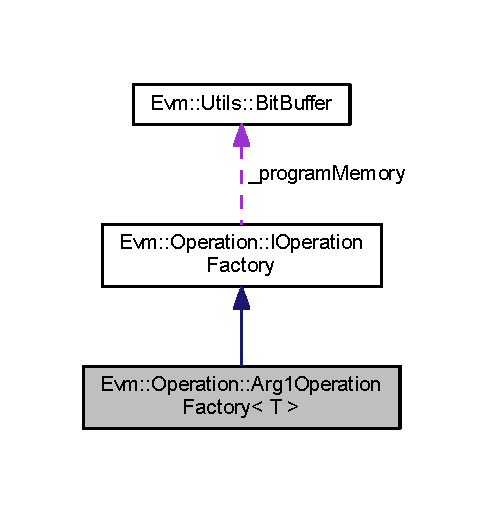
\includegraphics[width=235pt]{struct_evm_1_1_operation_1_1_arg1_operation_factory__coll__graph}
\end{center}
\end{figure}
\subsection*{Public Member Functions}
\begin{DoxyCompactItemize}
\item 
\mbox{\Hypertarget{struct_evm_1_1_operation_1_1_arg1_operation_factory_a9fb6cb8bd6676f2d20d73794545e17db}\label{struct_evm_1_1_operation_1_1_arg1_operation_factory_a9fb6cb8bd6676f2d20d73794545e17db}} 
virtual Operation\+Ptr {\bfseries build} (uint32\+\_\+t \&offset)
\item 
\mbox{\Hypertarget{struct_evm_1_1_operation_1_1_arg1_operation_factory_a7621b51ca2bc125b36be673486e33781}\label{struct_evm_1_1_operation_1_1_arg1_operation_factory_a7621b51ca2bc125b36be673486e33781}} 
{\bfseries I\+Operation\+Factory} (const string \&opcode, const \mbox{\hyperlink{struct_evm_1_1_utils_1_1_bit_buffer}{Utils\+::\+Bit\+Buffer}} \&program\+Memory)
\end{DoxyCompactItemize}
\subsection*{Additional Inherited Members}


The documentation for this struct was generated from the following file\+:\begin{DoxyCompactItemize}
\item 
Evm/Operation\+Factory.\+h\end{DoxyCompactItemize}

\hypertarget{struct_evm_1_1_bad_lock_i_d_runtime_error}{}\section{Evm\+:\+:Bad\+Lock\+I\+D\+Runtime\+Error Struct Reference}
\label{struct_evm_1_1_bad_lock_i_d_runtime_error}\index{Evm\+::\+Bad\+Lock\+I\+D\+Runtime\+Error@{Evm\+::\+Bad\+Lock\+I\+D\+Runtime\+Error}}


Inheritance diagram for Evm\+:\+:Bad\+Lock\+I\+D\+Runtime\+Error\+:
\nopagebreak
\begin{figure}[H]
\begin{center}
\leavevmode
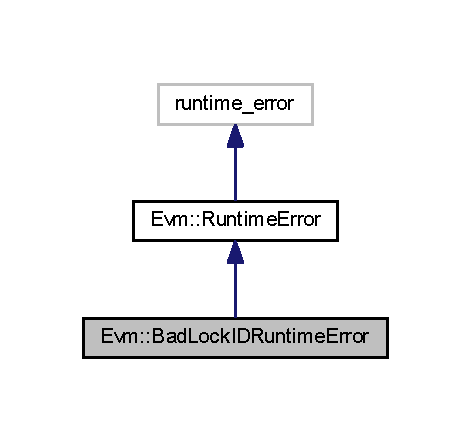
\includegraphics[width=226pt]{struct_evm_1_1_bad_lock_i_d_runtime_error__inherit__graph}
\end{center}
\end{figure}


Collaboration diagram for Evm\+:\+:Bad\+Lock\+I\+D\+Runtime\+Error\+:
\nopagebreak
\begin{figure}[H]
\begin{center}
\leavevmode
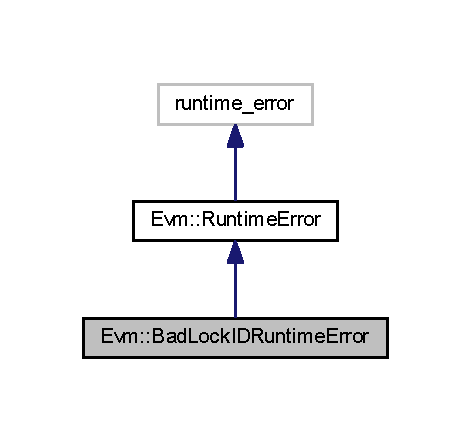
\includegraphics[width=226pt]{struct_evm_1_1_bad_lock_i_d_runtime_error__coll__graph}
\end{center}
\end{figure}
\subsection*{Public Member Functions}
\begin{DoxyCompactItemize}
\item 
\mbox{\Hypertarget{struct_evm_1_1_bad_lock_i_d_runtime_error_a5422087bc433fb211d48b3d827a32e89}\label{struct_evm_1_1_bad_lock_i_d_runtime_error_a5422087bc433fb211d48b3d827a32e89}} 
{\bfseries Bad\+Lock\+I\+D\+Runtime\+Error} (uint64\+\_\+t id)
\end{DoxyCompactItemize}


The documentation for this struct was generated from the following file\+:\begin{DoxyCompactItemize}
\item 
Evm/Runtime\+Error.\+h\end{DoxyCompactItemize}

\hypertarget{struct_evm_1_1_bad_register_runtime_error}{}\section{Evm\+:\+:Bad\+Register\+Runtime\+Error Struct Reference}
\label{struct_evm_1_1_bad_register_runtime_error}\index{Evm\+::\+Bad\+Register\+Runtime\+Error@{Evm\+::\+Bad\+Register\+Runtime\+Error}}


Inheritance diagram for Evm\+:\+:Bad\+Register\+Runtime\+Error\+:
\nopagebreak
\begin{figure}[H]
\begin{center}
\leavevmode
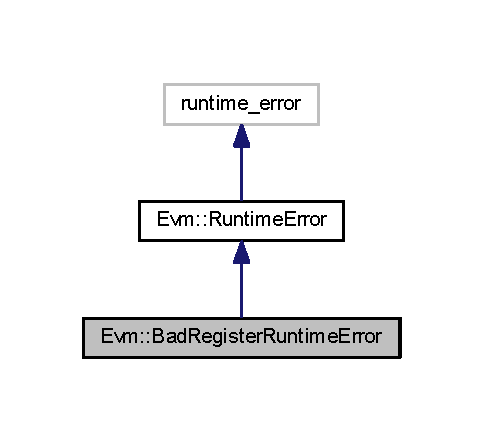
\includegraphics[width=232pt]{struct_evm_1_1_bad_register_runtime_error__inherit__graph}
\end{center}
\end{figure}


Collaboration diagram for Evm\+:\+:Bad\+Register\+Runtime\+Error\+:
\nopagebreak
\begin{figure}[H]
\begin{center}
\leavevmode
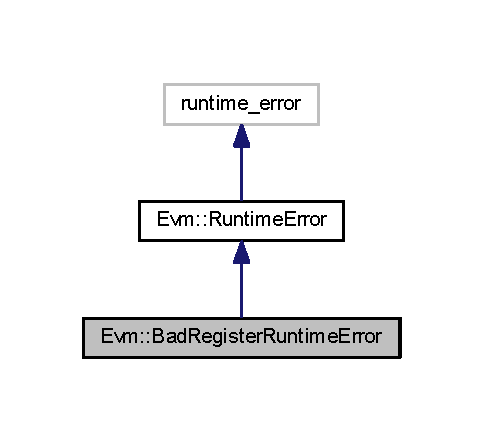
\includegraphics[width=232pt]{struct_evm_1_1_bad_register_runtime_error__coll__graph}
\end{center}
\end{figure}
\subsection*{Public Member Functions}
\begin{DoxyCompactItemize}
\item 
\mbox{\Hypertarget{struct_evm_1_1_bad_register_runtime_error_adab23c579d16fb4e9e327fdfbc3f7395}\label{struct_evm_1_1_bad_register_runtime_error_adab23c579d16fb4e9e327fdfbc3f7395}} 
{\bfseries Bad\+Register\+Runtime\+Error} (uint8\+\_\+t reg\+Index)
\end{DoxyCompactItemize}


The documentation for this struct was generated from the following file\+:\begin{DoxyCompactItemize}
\item 
Evm/Runtime\+Error.\+h\end{DoxyCompactItemize}

\hypertarget{struct_evm_1_1_utils_1_1_bit_buffer}{}\section{Evm\+:\+:Utils\+:\+:Bit\+Buffer Struct Reference}
\label{struct_evm_1_1_utils_1_1_bit_buffer}\index{Evm\+::\+Utils\+::\+Bit\+Buffer@{Evm\+::\+Utils\+::\+Bit\+Buffer}}
\subsection*{Public Member Functions}
\begin{DoxyCompactItemize}
\item 
\mbox{\Hypertarget{struct_evm_1_1_utils_1_1_bit_buffer_af62bf038f198244dcb02a97ebb31d0e1}\label{struct_evm_1_1_utils_1_1_bit_buffer_af62bf038f198244dcb02a97ebb31d0e1}} 
{\bfseries Bit\+Buffer} (const Bytes \&data)
\item 
\mbox{\Hypertarget{struct_evm_1_1_utils_1_1_bit_buffer_a83e441743de70d72d42e73733c7d76d4}\label{struct_evm_1_1_utils_1_1_bit_buffer_a83e441743de70d72d42e73733c7d76d4}} 
{\bfseries Bit\+Buffer} (Bytes\+::const\+\_\+iterator begin, Bytes\+::const\+\_\+iterator end)
\item 
\mbox{\Hypertarget{struct_evm_1_1_utils_1_1_bit_buffer_af0c9d384c109f2daa55e9c4a02dc332f}\label{struct_evm_1_1_utils_1_1_bit_buffer_af0c9d384c109f2daa55e9c4a02dc332f}} 
uint64\+\_\+t {\bfseries get\+U64} (uint32\+\_\+t bit\+Address, uint32\+\_\+t size, bool reversed=false) const
\item 
\mbox{\Hypertarget{struct_evm_1_1_utils_1_1_bit_buffer_a7727b3e57c89a4d55a513ec2ce75cc0b}\label{struct_evm_1_1_utils_1_1_bit_buffer_a7727b3e57c89a4d55a513ec2ce75cc0b}} 
uint32\+\_\+t {\bfseries get\+U32} (uint32\+\_\+t bit\+Address, uint32\+\_\+t size, bool reversed=false) const
\item 
\mbox{\Hypertarget{struct_evm_1_1_utils_1_1_bit_buffer_a06b8a0a12f532de218bc17cc3b1b97e2}\label{struct_evm_1_1_utils_1_1_bit_buffer_a06b8a0a12f532de218bc17cc3b1b97e2}} 
uint16\+\_\+t {\bfseries get\+U16} (uint32\+\_\+t bit\+Address, uint32\+\_\+t size, bool reversed=false) const
\item 
\mbox{\Hypertarget{struct_evm_1_1_utils_1_1_bit_buffer_ac6ecaf7a3617b9ea09c057d2d039100a}\label{struct_evm_1_1_utils_1_1_bit_buffer_ac6ecaf7a3617b9ea09c057d2d039100a}} 
uint8\+\_\+t {\bfseries get\+U8} (uint32\+\_\+t bit\+Address, uint32\+\_\+t size, bool reversed=false) const
\item 
\mbox{\Hypertarget{struct_evm_1_1_utils_1_1_bit_buffer_a1f58c76a7bdb52e1fa4ff244c137de10}\label{struct_evm_1_1_utils_1_1_bit_buffer_a1f58c76a7bdb52e1fa4ff244c137de10}} 
uint32\+\_\+t {\bfseries size} () const
\end{DoxyCompactItemize}


The documentation for this struct was generated from the following files\+:\begin{DoxyCompactItemize}
\item 
Evm/Bit\+Buffer.\+h\item 
Evm/Bit\+Buffer.\+cpp\end{DoxyCompactItemize}

\hypertarget{struct_evm_1_1_operation_1_1_call_operation}{}\section{Evm\+:\+:Operation\+:\+:Call\+Operation Struct Reference}
\label{struct_evm_1_1_operation_1_1_call_operation}\index{Evm\+::\+Operation\+::\+Call\+Operation@{Evm\+::\+Operation\+::\+Call\+Operation}}


call operation  




{\ttfamily \#include $<$Operation.\+h$>$}



Inheritance diagram for Evm\+:\+:Operation\+:\+:Call\+Operation\+:
\nopagebreak
\begin{figure}[H]
\begin{center}
\leavevmode
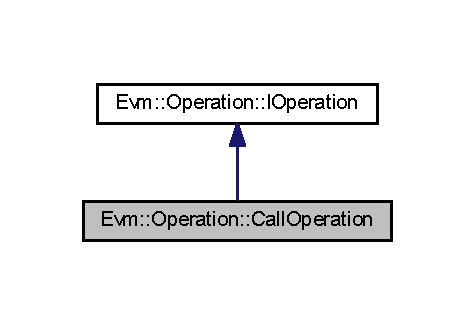
\includegraphics[width=228pt]{struct_evm_1_1_operation_1_1_call_operation__inherit__graph}
\end{center}
\end{figure}


Collaboration diagram for Evm\+:\+:Operation\+:\+:Call\+Operation\+:
\nopagebreak
\begin{figure}[H]
\begin{center}
\leavevmode
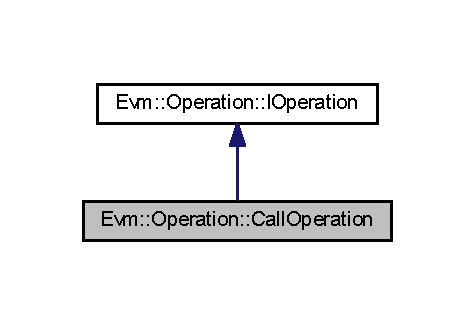
\includegraphics[width=228pt]{struct_evm_1_1_operation_1_1_call_operation__coll__graph}
\end{center}
\end{figure}
\subsection*{Public Member Functions}
\begin{DoxyCompactItemize}
\item 
virtual void \mbox{\hyperlink{struct_evm_1_1_operation_1_1_call_operation_ace9fbeb98abf5de426629be6eec22fd2}{execute}} (\mbox{\hyperlink{struct_evm_1_1_thread_context}{Thread\+Context}} \&thread) override
\begin{DoxyCompactList}\small\item\em Execution of the instruction. \end{DoxyCompactList}\item 
\mbox{\hyperlink{struct_evm_1_1_operation_1_1_call_operation_a65e98ee1b1679e12c1d1dd000ebfe937}{I\+Operation}} (string \&opcode)
\begin{DoxyCompactList}\small\item\em Constructor. \end{DoxyCompactList}\end{DoxyCompactItemize}
\subsection*{Additional Inherited Members}


\subsection{Detailed Description}
call operation 

call address; Store address of instruction after the call to internal stack and continue execution at address 

\subsection{Member Function Documentation}
\mbox{\Hypertarget{struct_evm_1_1_operation_1_1_call_operation_ace9fbeb98abf5de426629be6eec22fd2}\label{struct_evm_1_1_operation_1_1_call_operation_ace9fbeb98abf5de426629be6eec22fd2}} 
\index{Evm\+::\+Operation\+::\+Call\+Operation@{Evm\+::\+Operation\+::\+Call\+Operation}!execute@{execute}}
\index{execute@{execute}!Evm\+::\+Operation\+::\+Call\+Operation@{Evm\+::\+Operation\+::\+Call\+Operation}}
\subsubsection{\texorpdfstring{execute()}{execute()}}
{\footnotesize\ttfamily void Evm\+::\+Operation\+::\+Call\+Operation\+::execute (\begin{DoxyParamCaption}\item[{\mbox{\hyperlink{struct_evm_1_1_thread_context}{Thread\+Context}} \&}]{thread }\end{DoxyParamCaption})\hspace{0.3cm}{\ttfamily [override]}, {\ttfamily [virtual]}}



Execution of the instruction. 

May by call by an application to execute the operation. The execution requires to be awared of thread context within the operation is executed. 
\begin{DoxyParams}{Parameters}
{\em thread} & Context of \mbox{\hyperlink{namespace_evm}{Evm}} thread \\
\hline
\end{DoxyParams}


Implements \mbox{\hyperlink{struct_evm_1_1_operation_1_1_i_operation_a7285631335da103423c01471dedeb1d7}{Evm\+::\+Operation\+::\+I\+Operation}}.

\mbox{\Hypertarget{struct_evm_1_1_operation_1_1_call_operation_a65e98ee1b1679e12c1d1dd000ebfe937}\label{struct_evm_1_1_operation_1_1_call_operation_a65e98ee1b1679e12c1d1dd000ebfe937}} 
\index{Evm\+::\+Operation\+::\+Call\+Operation@{Evm\+::\+Operation\+::\+Call\+Operation}!I\+Operation@{I\+Operation}}
\index{I\+Operation@{I\+Operation}!Evm\+::\+Operation\+::\+Call\+Operation@{Evm\+::\+Operation\+::\+Call\+Operation}}
\subsubsection{\texorpdfstring{I\+Operation()}{IOperation()}}
{\footnotesize\ttfamily Evm\+::\+Operation\+::\+I\+Operation\+::\+I\+Operation\hspace{0.3cm}{\ttfamily [inline]}}



Constructor. 


\begin{DoxyParams}{Parameters}
{\em opcode} & Printable label of the instruction \\
\hline
\end{DoxyParams}


The documentation for this struct was generated from the following files\+:\begin{DoxyCompactItemize}
\item 
Evm/Operation.\+h\item 
Evm/\mbox{\hyperlink{_operation_8cpp}{Operation.\+cpp}}\end{DoxyCompactItemize}

\hypertarget{struct_evm_1_1_cli_configuration}{}\section{Evm\+:\+:Cli\+Configuration Struct Reference}
\label{struct_evm_1_1_cli_configuration}\index{Evm\+::\+Cli\+Configuration@{Evm\+::\+Cli\+Configuration}}


\mbox{\hyperlink{namespace_evm}{Evm}} configuration.  




{\ttfamily \#include $<$Application.\+h$>$}

\subsection*{Public Attributes}
\begin{DoxyCompactItemize}
\item 
\mbox{\Hypertarget{struct_evm_1_1_cli_configuration_aa63df356e835bc53792a7af4125945a9}\label{struct_evm_1_1_cli_configuration_aa63df356e835bc53792a7af4125945a9}} 
string \mbox{\hyperlink{struct_evm_1_1_cli_configuration_aa63df356e835bc53792a7af4125945a9}{evm\+File\+Name}}
\begin{DoxyCompactList}\small\item\em File name of .evm executable. \end{DoxyCompactList}\item 
\mbox{\Hypertarget{struct_evm_1_1_cli_configuration_a98c1b5af8263e6208ec9b2bc2cfe595e}\label{struct_evm_1_1_cli_configuration_a98c1b5af8263e6208ec9b2bc2cfe595e}} 
string \mbox{\hyperlink{struct_evm_1_1_cli_configuration_a98c1b5af8263e6208ec9b2bc2cfe595e}{input\+File\+Name}}
\begin{DoxyCompactList}\small\item\em File name of user input file (if it is required) \end{DoxyCompactList}\item 
\mbox{\Hypertarget{struct_evm_1_1_cli_configuration_adb445455ca905fb6dccb0c212f46ce51}\label{struct_evm_1_1_cli_configuration_adb445455ca905fb6dccb0c212f46ce51}} 
bool \mbox{\hyperlink{struct_evm_1_1_cli_configuration_adb445455ca905fb6dccb0c212f46ce51}{input\+File\+Is\+Given}}
\begin{DoxyCompactList}\small\item\em True if the input file is given. \end{DoxyCompactList}\item 
\mbox{\Hypertarget{struct_evm_1_1_cli_configuration_a0a296d97c4674e4f2460ffb85263552a}\label{struct_evm_1_1_cli_configuration_a0a296d97c4674e4f2460ffb85263552a}} 
bool \mbox{\hyperlink{struct_evm_1_1_cli_configuration_a0a296d97c4674e4f2460ffb85263552a}{trace}}
\begin{DoxyCompactList}\small\item\em True if command execution trace is enabled. \end{DoxyCompactList}\end{DoxyCompactItemize}


\subsection{Detailed Description}
\mbox{\hyperlink{namespace_evm}{Evm}} configuration. 

Configuration structure for \mbox{\hyperlink{namespace_evm}{Evm}} \mbox{\hyperlink{struct_evm_1_1_application}{Application}}. Can be filled by hand or captured from console by \mbox{\hyperlink{namespace_evm_aa2edd047bba5bfc0fd7bdf9d49538c16}{get\+Cli\+Configuration()}} 

The documentation for this struct was generated from the following file\+:\begin{DoxyCompactItemize}
\item 
Evm/\mbox{\hyperlink{_application_8h}{Application.\+h}}\end{DoxyCompactItemize}

\hypertarget{struct_evm_1_1_cli_configuration_runtime_error}{}\section{Evm\+:\+:Cli\+Configuration\+Runtime\+Error Struct Reference}
\label{struct_evm_1_1_cli_configuration_runtime_error}\index{Evm\+::\+Cli\+Configuration\+Runtime\+Error@{Evm\+::\+Cli\+Configuration\+Runtime\+Error}}


Inheritance diagram for Evm\+:\+:Cli\+Configuration\+Runtime\+Error\+:
\nopagebreak
\begin{figure}[H]
\begin{center}
\leavevmode
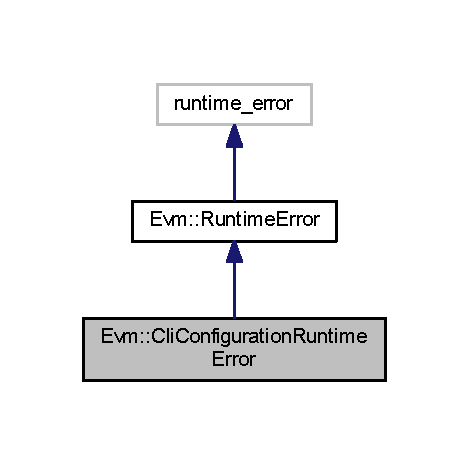
\includegraphics[width=225pt]{struct_evm_1_1_cli_configuration_runtime_error__inherit__graph}
\end{center}
\end{figure}


Collaboration diagram for Evm\+:\+:Cli\+Configuration\+Runtime\+Error\+:
\nopagebreak
\begin{figure}[H]
\begin{center}
\leavevmode
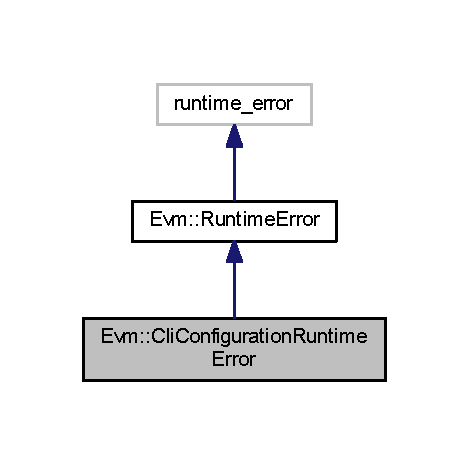
\includegraphics[width=225pt]{struct_evm_1_1_cli_configuration_runtime_error__coll__graph}
\end{center}
\end{figure}
\subsection*{Public Member Functions}
\begin{DoxyCompactItemize}
\item 
\mbox{\Hypertarget{struct_evm_1_1_cli_configuration_runtime_error_a8ae06332c5e8cd5e20c923ea5c0f7cec}\label{struct_evm_1_1_cli_configuration_runtime_error_a8ae06332c5e8cd5e20c923ea5c0f7cec}} 
{\bfseries Cli\+Configuration\+Runtime\+Error} (const string \&msg)
\end{DoxyCompactItemize}


The documentation for this struct was generated from the following file\+:\begin{DoxyCompactItemize}
\item 
Evm/Runtime\+Error.\+h\end{DoxyCompactItemize}

\hypertarget{struct_evm_1_1_operation_1_1_console_read_operation}{}\section{Evm\+:\+:Operation\+:\+:Console\+Read\+Operation Struct Reference}
\label{struct_evm_1_1_operation_1_1_console_read_operation}\index{Evm\+::\+Operation\+::\+Console\+Read\+Operation@{Evm\+::\+Operation\+::\+Console\+Read\+Operation}}


console\+Read operation  




{\ttfamily \#include $<$Operation.\+h$>$}



Inheritance diagram for Evm\+:\+:Operation\+:\+:Console\+Read\+Operation\+:
\nopagebreak
\begin{figure}[H]
\begin{center}
\leavevmode
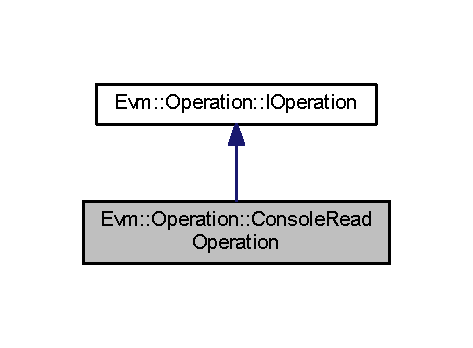
\includegraphics[width=227pt]{struct_evm_1_1_operation_1_1_console_read_operation__inherit__graph}
\end{center}
\end{figure}


Collaboration diagram for Evm\+:\+:Operation\+:\+:Console\+Read\+Operation\+:
\nopagebreak
\begin{figure}[H]
\begin{center}
\leavevmode
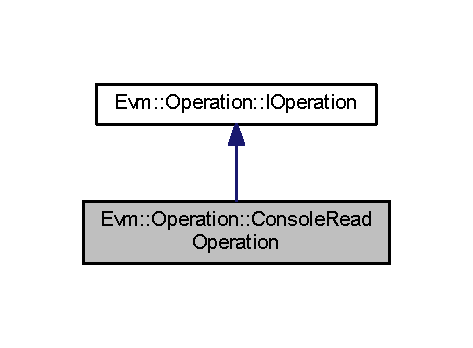
\includegraphics[width=227pt]{struct_evm_1_1_operation_1_1_console_read_operation__coll__graph}
\end{center}
\end{figure}
\subsection*{Public Member Functions}
\begin{DoxyCompactItemize}
\item 
virtual void \mbox{\hyperlink{struct_evm_1_1_operation_1_1_console_read_operation_a7bd7cfc2022abbb7fc9b45a2c75083e0}{execute}} (\mbox{\hyperlink{struct_evm_1_1_thread_context}{Thread\+Context}} \&thread) override
\begin{DoxyCompactList}\small\item\em Execution of the instruction. \end{DoxyCompactList}\item 
\mbox{\hyperlink{struct_evm_1_1_operation_1_1_console_read_operation_a65e98ee1b1679e12c1d1dd000ebfe937}{I\+Operation}} (string \&opcode)
\begin{DoxyCompactList}\small\item\em Constructor. \end{DoxyCompactList}\end{DoxyCompactItemize}
\subsection*{Additional Inherited Members}


\subsection{Detailed Description}
console\+Read operation 

console\+Read arg1; Read hexadecimal value from console and store to arg1 

\subsection{Member Function Documentation}
\mbox{\Hypertarget{struct_evm_1_1_operation_1_1_console_read_operation_a7bd7cfc2022abbb7fc9b45a2c75083e0}\label{struct_evm_1_1_operation_1_1_console_read_operation_a7bd7cfc2022abbb7fc9b45a2c75083e0}} 
\index{Evm\+::\+Operation\+::\+Console\+Read\+Operation@{Evm\+::\+Operation\+::\+Console\+Read\+Operation}!execute@{execute}}
\index{execute@{execute}!Evm\+::\+Operation\+::\+Console\+Read\+Operation@{Evm\+::\+Operation\+::\+Console\+Read\+Operation}}
\subsubsection{\texorpdfstring{execute()}{execute()}}
{\footnotesize\ttfamily void Evm\+::\+Operation\+::\+Console\+Read\+Operation\+::execute (\begin{DoxyParamCaption}\item[{\mbox{\hyperlink{struct_evm_1_1_thread_context}{Thread\+Context}} \&}]{thread }\end{DoxyParamCaption})\hspace{0.3cm}{\ttfamily [override]}, {\ttfamily [virtual]}}



Execution of the instruction. 

May by call by an application to execute the operation. The execution requires to be awared of thread context within the operation is executed. 
\begin{DoxyParams}{Parameters}
{\em thread} & Context of \mbox{\hyperlink{namespace_evm}{Evm}} thread \\
\hline
\end{DoxyParams}


Implements \mbox{\hyperlink{struct_evm_1_1_operation_1_1_i_operation_a7285631335da103423c01471dedeb1d7}{Evm\+::\+Operation\+::\+I\+Operation}}.

\mbox{\Hypertarget{struct_evm_1_1_operation_1_1_console_read_operation_a65e98ee1b1679e12c1d1dd000ebfe937}\label{struct_evm_1_1_operation_1_1_console_read_operation_a65e98ee1b1679e12c1d1dd000ebfe937}} 
\index{Evm\+::\+Operation\+::\+Console\+Read\+Operation@{Evm\+::\+Operation\+::\+Console\+Read\+Operation}!I\+Operation@{I\+Operation}}
\index{I\+Operation@{I\+Operation}!Evm\+::\+Operation\+::\+Console\+Read\+Operation@{Evm\+::\+Operation\+::\+Console\+Read\+Operation}}
\subsubsection{\texorpdfstring{I\+Operation()}{IOperation()}}
{\footnotesize\ttfamily Evm\+::\+Operation\+::\+I\+Operation\+::\+I\+Operation\hspace{0.3cm}{\ttfamily [inline]}}



Constructor. 


\begin{DoxyParams}{Parameters}
{\em opcode} & Printable label of the instruction \\
\hline
\end{DoxyParams}


The documentation for this struct was generated from the following files\+:\begin{DoxyCompactItemize}
\item 
Evm/Operation.\+h\item 
Evm/\mbox{\hyperlink{_operation_8cpp}{Operation.\+cpp}}\end{DoxyCompactItemize}

\hypertarget{struct_evm_1_1_operation_1_1_console_write_operation}{}\section{Evm\+:\+:Operation\+:\+:Console\+Write\+Operation Struct Reference}
\label{struct_evm_1_1_operation_1_1_console_write_operation}\index{Evm\+::\+Operation\+::\+Console\+Write\+Operation@{Evm\+::\+Operation\+::\+Console\+Write\+Operation}}


console\+Write operation  




{\ttfamily \#include $<$Operation.\+h$>$}



Inheritance diagram for Evm\+:\+:Operation\+:\+:Console\+Write\+Operation\+:
\nopagebreak
\begin{figure}[H]
\begin{center}
\leavevmode
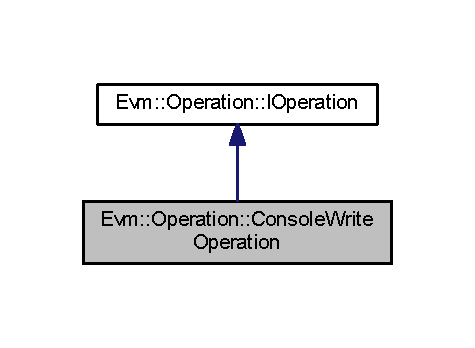
\includegraphics[width=228pt]{struct_evm_1_1_operation_1_1_console_write_operation__inherit__graph}
\end{center}
\end{figure}


Collaboration diagram for Evm\+:\+:Operation\+:\+:Console\+Write\+Operation\+:
\nopagebreak
\begin{figure}[H]
\begin{center}
\leavevmode
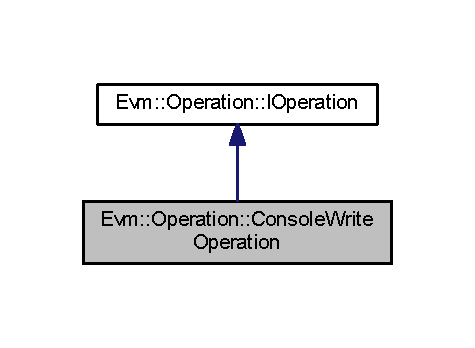
\includegraphics[width=228pt]{struct_evm_1_1_operation_1_1_console_write_operation__coll__graph}
\end{center}
\end{figure}
\subsection*{Public Member Functions}
\begin{DoxyCompactItemize}
\item 
virtual void \mbox{\hyperlink{struct_evm_1_1_operation_1_1_console_write_operation_a5dc059cb2b6faacc3dd1b477eec645e1}{execute}} (\mbox{\hyperlink{struct_evm_1_1_thread_context}{Thread\+Context}} \&thread) override
\begin{DoxyCompactList}\small\item\em Execution of the instruction. \end{DoxyCompactList}\item 
\mbox{\hyperlink{struct_evm_1_1_operation_1_1_console_write_operation_a65e98ee1b1679e12c1d1dd000ebfe937}{I\+Operation}} (string \&opcode)
\begin{DoxyCompactList}\small\item\em Constructor. \end{DoxyCompactList}\end{DoxyCompactItemize}
\subsection*{Additional Inherited Members}


\subsection{Detailed Description}
console\+Write operation 

console\+Write arg1; Write arg1 to console, as hexadecimal value. 

\subsection{Member Function Documentation}
\mbox{\Hypertarget{struct_evm_1_1_operation_1_1_console_write_operation_a5dc059cb2b6faacc3dd1b477eec645e1}\label{struct_evm_1_1_operation_1_1_console_write_operation_a5dc059cb2b6faacc3dd1b477eec645e1}} 
\index{Evm\+::\+Operation\+::\+Console\+Write\+Operation@{Evm\+::\+Operation\+::\+Console\+Write\+Operation}!execute@{execute}}
\index{execute@{execute}!Evm\+::\+Operation\+::\+Console\+Write\+Operation@{Evm\+::\+Operation\+::\+Console\+Write\+Operation}}
\subsubsection{\texorpdfstring{execute()}{execute()}}
{\footnotesize\ttfamily void Evm\+::\+Operation\+::\+Console\+Write\+Operation\+::execute (\begin{DoxyParamCaption}\item[{\mbox{\hyperlink{struct_evm_1_1_thread_context}{Thread\+Context}} \&}]{thread }\end{DoxyParamCaption})\hspace{0.3cm}{\ttfamily [override]}, {\ttfamily [virtual]}}



Execution of the instruction. 

May by call by an application to execute the operation. The execution requires to be awared of thread context within the operation is executed. 
\begin{DoxyParams}{Parameters}
{\em thread} & Context of \mbox{\hyperlink{namespace_evm}{Evm}} thread \\
\hline
\end{DoxyParams}


Implements \mbox{\hyperlink{struct_evm_1_1_operation_1_1_i_operation_a7285631335da103423c01471dedeb1d7}{Evm\+::\+Operation\+::\+I\+Operation}}.

\mbox{\Hypertarget{struct_evm_1_1_operation_1_1_console_write_operation_a65e98ee1b1679e12c1d1dd000ebfe937}\label{struct_evm_1_1_operation_1_1_console_write_operation_a65e98ee1b1679e12c1d1dd000ebfe937}} 
\index{Evm\+::\+Operation\+::\+Console\+Write\+Operation@{Evm\+::\+Operation\+::\+Console\+Write\+Operation}!I\+Operation@{I\+Operation}}
\index{I\+Operation@{I\+Operation}!Evm\+::\+Operation\+::\+Console\+Write\+Operation@{Evm\+::\+Operation\+::\+Console\+Write\+Operation}}
\subsubsection{\texorpdfstring{I\+Operation()}{IOperation()}}
{\footnotesize\ttfamily Evm\+::\+Operation\+::\+I\+Operation\+::\+I\+Operation\hspace{0.3cm}{\ttfamily [inline]}}



Constructor. 


\begin{DoxyParams}{Parameters}
{\em opcode} & Printable label of the instruction \\
\hline
\end{DoxyParams}


The documentation for this struct was generated from the following files\+:\begin{DoxyCompactItemize}
\item 
Evm/Operation.\+h\item 
Evm/\mbox{\hyperlink{_operation_8cpp}{Operation.\+cpp}}\end{DoxyCompactItemize}

\hypertarget{struct_evm_1_1_argument_1_1_const_argument}{}\section{Evm\+:\+:Argument\+:\+:Const\+Argument Struct Reference}
\label{struct_evm_1_1_argument_1_1_const_argument}\index{Evm\+::\+Argument\+::\+Const\+Argument@{Evm\+::\+Argument\+::\+Const\+Argument}}


Inheritance diagram for Evm\+:\+:Argument\+:\+:Const\+Argument\+:
\nopagebreak
\begin{figure}[H]
\begin{center}
\leavevmode
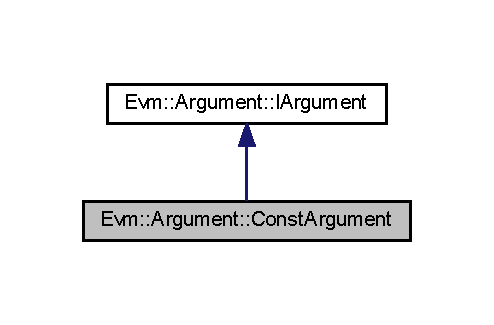
\includegraphics[width=237pt]{struct_evm_1_1_argument_1_1_const_argument__inherit__graph}
\end{center}
\end{figure}


Collaboration diagram for Evm\+:\+:Argument\+:\+:Const\+Argument\+:
\nopagebreak
\begin{figure}[H]
\begin{center}
\leavevmode
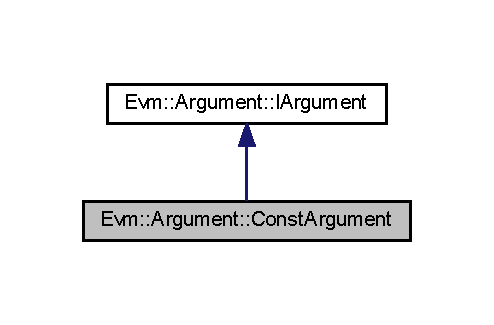
\includegraphics[width=237pt]{struct_evm_1_1_argument_1_1_const_argument__coll__graph}
\end{center}
\end{figure}
\subsection*{Public Member Functions}
\begin{DoxyCompactItemize}
\item 
\mbox{\Hypertarget{struct_evm_1_1_argument_1_1_const_argument_a58766ea5cf2f90482407c040b9d78d5d}\label{struct_evm_1_1_argument_1_1_const_argument_a58766ea5cf2f90482407c040b9d78d5d}} 
{\bfseries Const\+Argument} (uint64\+\_\+t const\+Value)
\item 
virtual uint64\+\_\+t \mbox{\hyperlink{struct_evm_1_1_argument_1_1_const_argument_abd4e5bb5fdad5eb9bd76436ea9c6836c}{get\+Value}} (\mbox{\hyperlink{struct_evm_1_1_thread_context}{Thread\+Context}} \&thread) const override
\begin{DoxyCompactList}\small\item\em Get value. \end{DoxyCompactList}\item 
virtual void \mbox{\hyperlink{struct_evm_1_1_argument_1_1_const_argument_ab456fa9175551b4c04815ccd65c76bd2}{set\+Value}} (\mbox{\hyperlink{struct_evm_1_1_thread_context}{Thread\+Context}} \&thread, uint64\+\_\+t value) override
\begin{DoxyCompactList}\small\item\em Set value. \end{DoxyCompactList}\item 
virtual string \mbox{\hyperlink{struct_evm_1_1_argument_1_1_const_argument_a90801800ff37e785e946f077f1c486f6}{label}} () const override
\begin{DoxyCompactList}\small\item\em Get printable representation of the argument. \end{DoxyCompactList}\item 
virtual string \mbox{\hyperlink{struct_evm_1_1_argument_1_1_const_argument_a5741f701088fadebf19b733c6973898b}{print\+Value}} (\mbox{\hyperlink{struct_evm_1_1_thread_context}{Thread\+Context}} \&thread) const override
\begin{DoxyCompactList}\small\item\em Get printable value of the parameter. \end{DoxyCompactList}\end{DoxyCompactItemize}


\subsection{Member Function Documentation}
\mbox{\Hypertarget{struct_evm_1_1_argument_1_1_const_argument_abd4e5bb5fdad5eb9bd76436ea9c6836c}\label{struct_evm_1_1_argument_1_1_const_argument_abd4e5bb5fdad5eb9bd76436ea9c6836c}} 
\index{Evm\+::\+Argument\+::\+Const\+Argument@{Evm\+::\+Argument\+::\+Const\+Argument}!get\+Value@{get\+Value}}
\index{get\+Value@{get\+Value}!Evm\+::\+Argument\+::\+Const\+Argument@{Evm\+::\+Argument\+::\+Const\+Argument}}
\subsubsection{\texorpdfstring{get\+Value()}{getValue()}}
{\footnotesize\ttfamily uint64\+\_\+t Evm\+::\+Argument\+::\+Const\+Argument\+::get\+Value (\begin{DoxyParamCaption}\item[{\mbox{\hyperlink{struct_evm_1_1_thread_context}{Thread\+Context}} \&}]{thread }\end{DoxyParamCaption}) const\hspace{0.3cm}{\ttfamily [override]}, {\ttfamily [virtual]}}



Get value. 

Return value of the argument 
\begin{DoxyParams}{Parameters}
{\em thread} & Thread context within this argument is used \\
\hline
\end{DoxyParams}
\begin{DoxyReturn}{Returns}
Value of the parameter 
\end{DoxyReturn}


Implements \mbox{\hyperlink{struct_evm_1_1_argument_1_1_i_argument_af01db10f34498344831877847c2fc038}{Evm\+::\+Argument\+::\+I\+Argument}}.

\mbox{\Hypertarget{struct_evm_1_1_argument_1_1_const_argument_a90801800ff37e785e946f077f1c486f6}\label{struct_evm_1_1_argument_1_1_const_argument_a90801800ff37e785e946f077f1c486f6}} 
\index{Evm\+::\+Argument\+::\+Const\+Argument@{Evm\+::\+Argument\+::\+Const\+Argument}!label@{label}}
\index{label@{label}!Evm\+::\+Argument\+::\+Const\+Argument@{Evm\+::\+Argument\+::\+Const\+Argument}}
\subsubsection{\texorpdfstring{label()}{label()}}
{\footnotesize\ttfamily string Evm\+::\+Argument\+::\+Const\+Argument\+::label (\begin{DoxyParamCaption}{ }\end{DoxyParamCaption}) const\hspace{0.3cm}{\ttfamily [override]}, {\ttfamily [virtual]}}



Get printable representation of the argument. 

\begin{DoxyReturn}{Returns}
string with argument label 
\end{DoxyReturn}


Implements \mbox{\hyperlink{struct_evm_1_1_argument_1_1_i_argument_a35bdae816e89f6f9fc393b6e03c5e521}{Evm\+::\+Argument\+::\+I\+Argument}}.

\mbox{\Hypertarget{struct_evm_1_1_argument_1_1_const_argument_a5741f701088fadebf19b733c6973898b}\label{struct_evm_1_1_argument_1_1_const_argument_a5741f701088fadebf19b733c6973898b}} 
\index{Evm\+::\+Argument\+::\+Const\+Argument@{Evm\+::\+Argument\+::\+Const\+Argument}!print\+Value@{print\+Value}}
\index{print\+Value@{print\+Value}!Evm\+::\+Argument\+::\+Const\+Argument@{Evm\+::\+Argument\+::\+Const\+Argument}}
\subsubsection{\texorpdfstring{print\+Value()}{printValue()}}
{\footnotesize\ttfamily string Evm\+::\+Argument\+::\+Const\+Argument\+::print\+Value (\begin{DoxyParamCaption}\item[{\mbox{\hyperlink{struct_evm_1_1_thread_context}{Thread\+Context}} \&}]{thread }\end{DoxyParamCaption}) const\hspace{0.3cm}{\ttfamily [override]}, {\ttfamily [virtual]}}



Get printable value of the parameter. 


\begin{DoxyParams}{Parameters}
{\em thread} & Thread context within this argument is used \\
\hline
\end{DoxyParams}
\begin{DoxyReturn}{Returns}
string with argument value 
\end{DoxyReturn}


Implements \mbox{\hyperlink{struct_evm_1_1_argument_1_1_i_argument_afcab2d2a1515518a111881a635c83da3}{Evm\+::\+Argument\+::\+I\+Argument}}.

\mbox{\Hypertarget{struct_evm_1_1_argument_1_1_const_argument_ab456fa9175551b4c04815ccd65c76bd2}\label{struct_evm_1_1_argument_1_1_const_argument_ab456fa9175551b4c04815ccd65c76bd2}} 
\index{Evm\+::\+Argument\+::\+Const\+Argument@{Evm\+::\+Argument\+::\+Const\+Argument}!set\+Value@{set\+Value}}
\index{set\+Value@{set\+Value}!Evm\+::\+Argument\+::\+Const\+Argument@{Evm\+::\+Argument\+::\+Const\+Argument}}
\subsubsection{\texorpdfstring{set\+Value()}{setValue()}}
{\footnotesize\ttfamily void Evm\+::\+Argument\+::\+Const\+Argument\+::set\+Value (\begin{DoxyParamCaption}\item[{\mbox{\hyperlink{struct_evm_1_1_thread_context}{Thread\+Context}} \&}]{thread,  }\item[{uint64\+\_\+t}]{value }\end{DoxyParamCaption})\hspace{0.3cm}{\ttfamily [override]}, {\ttfamily [virtual]}}



Set value. 

Set value of the argument. \begin{DoxyWarning}{Warning}
For read-\/only arguments this throws an exception 
\end{DoxyWarning}

\begin{DoxyParams}{Parameters}
{\em thread} & Thread context within this argument is used \\
\hline
{\em value} & New value of the parameter \\
\hline
\end{DoxyParams}


Implements \mbox{\hyperlink{struct_evm_1_1_argument_1_1_i_argument_a24e4c76f2750e664e3895d2ff4b9146d}{Evm\+::\+Argument\+::\+I\+Argument}}.



The documentation for this struct was generated from the following files\+:\begin{DoxyCompactItemize}
\item 
Evm/\mbox{\hyperlink{_argument_8h}{Argument.\+h}}\item 
Evm/Argument.\+cpp\end{DoxyCompactItemize}

\hypertarget{union_evm_1_1_argument_1_1_convert_union}{}\section{Evm\+:\+:Argument\+:\+:Convert\+Union Union Reference}
\label{union_evm_1_1_argument_1_1_convert_union}\index{Evm\+::\+Argument\+::\+Convert\+Union@{Evm\+::\+Argument\+::\+Convert\+Union}}
\subsection*{Public Attributes}
\begin{DoxyCompactItemize}
\item 
\mbox{\Hypertarget{union_evm_1_1_argument_1_1_convert_union_af260a152260e9dce301b3c2256b2f5ce}\label{union_evm_1_1_argument_1_1_convert_union_af260a152260e9dce301b3c2256b2f5ce}} 
uint64\+\_\+t {\bfseries u64}
\item 
\mbox{\Hypertarget{union_evm_1_1_argument_1_1_convert_union_abe47d441d4b7958434093b7c204fffd4}\label{union_evm_1_1_argument_1_1_convert_union_abe47d441d4b7958434093b7c204fffd4}} 
uint32\+\_\+t {\bfseries u32} \mbox{[}2\mbox{]}
\item 
\mbox{\Hypertarget{union_evm_1_1_argument_1_1_convert_union_ac9dc1da78775f62b92dbca1c0861ef2a}\label{union_evm_1_1_argument_1_1_convert_union_ac9dc1da78775f62b92dbca1c0861ef2a}} 
uint16\+\_\+t {\bfseries u16} \mbox{[}4\mbox{]}
\item 
\mbox{\Hypertarget{union_evm_1_1_argument_1_1_convert_union_a40fe62a842931fcd9a0ac406dedf6686}\label{union_evm_1_1_argument_1_1_convert_union_a40fe62a842931fcd9a0ac406dedf6686}} 
uint8\+\_\+t {\bfseries u8} \mbox{[}8\mbox{]}
\end{DoxyCompactItemize}


The documentation for this union was generated from the following file\+:\begin{DoxyCompactItemize}
\item 
Evm/Argument.\+cpp\end{DoxyCompactItemize}

\hypertarget{struct_evm_1_1_operation_1_1_create_thread_operation}{}\section{Evm\+:\+:Operation\+:\+:Create\+Thread\+Operation Struct Reference}
\label{struct_evm_1_1_operation_1_1_create_thread_operation}\index{Evm\+::\+Operation\+::\+Create\+Thread\+Operation@{Evm\+::\+Operation\+::\+Create\+Thread\+Operation}}


create\+Thread operation  




{\ttfamily \#include $<$Operation.\+h$>$}



Inheritance diagram for Evm\+:\+:Operation\+:\+:Create\+Thread\+Operation\+:
\nopagebreak
\begin{figure}[H]
\begin{center}
\leavevmode
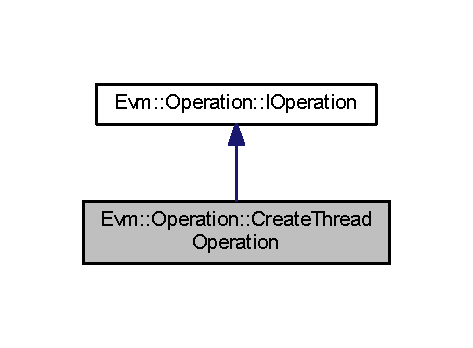
\includegraphics[width=227pt]{struct_evm_1_1_operation_1_1_create_thread_operation__inherit__graph}
\end{center}
\end{figure}


Collaboration diagram for Evm\+:\+:Operation\+:\+:Create\+Thread\+Operation\+:
\nopagebreak
\begin{figure}[H]
\begin{center}
\leavevmode
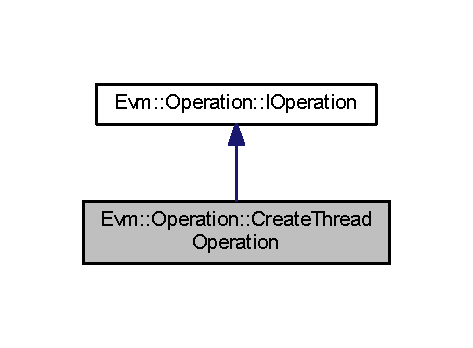
\includegraphics[width=227pt]{struct_evm_1_1_operation_1_1_create_thread_operation__coll__graph}
\end{center}
\end{figure}
\subsection*{Public Member Functions}
\begin{DoxyCompactItemize}
\item 
virtual void \mbox{\hyperlink{struct_evm_1_1_operation_1_1_create_thread_operation_a5efc82f864a95f07bd4312522cd91c70}{execute}} (\mbox{\hyperlink{struct_evm_1_1_thread_context}{Thread\+Context}} \&thread) override
\begin{DoxyCompactList}\small\item\em Execution of the instruction. \end{DoxyCompactList}\item 
\mbox{\hyperlink{struct_evm_1_1_operation_1_1_create_thread_operation_a65e98ee1b1679e12c1d1dd000ebfe937}{I\+Operation}} (string \&opcode)
\begin{DoxyCompactList}\small\item\em Constructor. \end{DoxyCompactList}\end{DoxyCompactItemize}
\subsection*{Additional Inherited Members}


\subsection{Detailed Description}
create\+Thread operation 

create\+Thread address, arg1; Create a new thread, starting at address and store it�s identifier to arg1. New thread starts with copy of current thread�s registers. 

\subsection{Member Function Documentation}
\mbox{\Hypertarget{struct_evm_1_1_operation_1_1_create_thread_operation_a5efc82f864a95f07bd4312522cd91c70}\label{struct_evm_1_1_operation_1_1_create_thread_operation_a5efc82f864a95f07bd4312522cd91c70}} 
\index{Evm\+::\+Operation\+::\+Create\+Thread\+Operation@{Evm\+::\+Operation\+::\+Create\+Thread\+Operation}!execute@{execute}}
\index{execute@{execute}!Evm\+::\+Operation\+::\+Create\+Thread\+Operation@{Evm\+::\+Operation\+::\+Create\+Thread\+Operation}}
\subsubsection{\texorpdfstring{execute()}{execute()}}
{\footnotesize\ttfamily void Evm\+::\+Operation\+::\+Create\+Thread\+Operation\+::execute (\begin{DoxyParamCaption}\item[{\mbox{\hyperlink{struct_evm_1_1_thread_context}{Thread\+Context}} \&}]{thread }\end{DoxyParamCaption})\hspace{0.3cm}{\ttfamily [override]}, {\ttfamily [virtual]}}



Execution of the instruction. 

May by call by an application to execute the operation. The execution requires to be awared of thread context within the operation is executed. 
\begin{DoxyParams}{Parameters}
{\em thread} & Context of \mbox{\hyperlink{namespace_evm}{Evm}} thread \\
\hline
\end{DoxyParams}


Implements \mbox{\hyperlink{struct_evm_1_1_operation_1_1_i_operation_a7285631335da103423c01471dedeb1d7}{Evm\+::\+Operation\+::\+I\+Operation}}.

\mbox{\Hypertarget{struct_evm_1_1_operation_1_1_create_thread_operation_a65e98ee1b1679e12c1d1dd000ebfe937}\label{struct_evm_1_1_operation_1_1_create_thread_operation_a65e98ee1b1679e12c1d1dd000ebfe937}} 
\index{Evm\+::\+Operation\+::\+Create\+Thread\+Operation@{Evm\+::\+Operation\+::\+Create\+Thread\+Operation}!I\+Operation@{I\+Operation}}
\index{I\+Operation@{I\+Operation}!Evm\+::\+Operation\+::\+Create\+Thread\+Operation@{Evm\+::\+Operation\+::\+Create\+Thread\+Operation}}
\subsubsection{\texorpdfstring{I\+Operation()}{IOperation()}}
{\footnotesize\ttfamily Evm\+::\+Operation\+::\+I\+Operation\+::\+I\+Operation\hspace{0.3cm}{\ttfamily [inline]}}



Constructor. 


\begin{DoxyParams}{Parameters}
{\em opcode} & Printable label of the instruction \\
\hline
\end{DoxyParams}


The documentation for this struct was generated from the following files\+:\begin{DoxyCompactItemize}
\item 
Evm/Operation.\+h\item 
Evm/\mbox{\hyperlink{_operation_8cpp}{Operation.\+cpp}}\end{DoxyCompactItemize}

\hypertarget{struct_evm_1_1_operation_1_1_create_thread_operation_factory}{}\section{Evm\+:\+:Operation\+:\+:Create\+Thread\+Operation\+Factory Struct Reference}
\label{struct_evm_1_1_operation_1_1_create_thread_operation_factory}\index{Evm\+::\+Operation\+::\+Create\+Thread\+Operation\+Factory@{Evm\+::\+Operation\+::\+Create\+Thread\+Operation\+Factory}}


Inheritance diagram for Evm\+:\+:Operation\+:\+:Create\+Thread\+Operation\+Factory\+:
\nopagebreak
\begin{figure}[H]
\begin{center}
\leavevmode
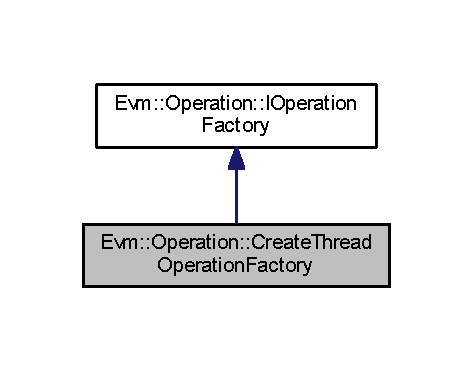
\includegraphics[width=227pt]{struct_evm_1_1_operation_1_1_create_thread_operation_factory__inherit__graph}
\end{center}
\end{figure}


Collaboration diagram for Evm\+:\+:Operation\+:\+:Create\+Thread\+Operation\+Factory\+:
\nopagebreak
\begin{figure}[H]
\begin{center}
\leavevmode
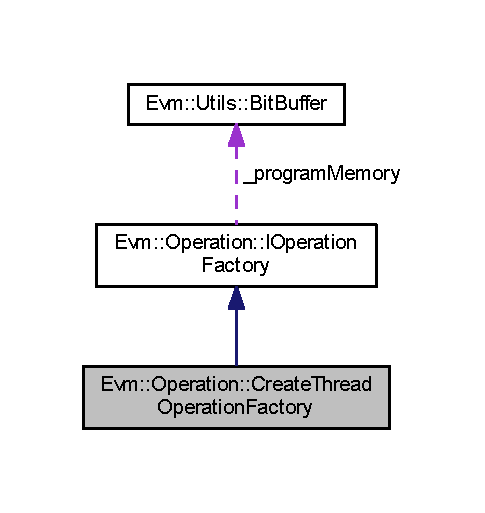
\includegraphics[width=233pt]{struct_evm_1_1_operation_1_1_create_thread_operation_factory__coll__graph}
\end{center}
\end{figure}
\subsection*{Public Member Functions}
\begin{DoxyCompactItemize}
\item 
\mbox{\Hypertarget{struct_evm_1_1_operation_1_1_create_thread_operation_factory_af6b5055ba3c732138cd2a276e0a9486b}\label{struct_evm_1_1_operation_1_1_create_thread_operation_factory_af6b5055ba3c732138cd2a276e0a9486b}} 
virtual Operation\+Ptr {\bfseries build} (uint32\+\_\+t \&offset)
\item 
\mbox{\Hypertarget{struct_evm_1_1_operation_1_1_create_thread_operation_factory_a7621b51ca2bc125b36be673486e33781}\label{struct_evm_1_1_operation_1_1_create_thread_operation_factory_a7621b51ca2bc125b36be673486e33781}} 
{\bfseries I\+Operation\+Factory} (const string \&opcode, const \mbox{\hyperlink{struct_evm_1_1_utils_1_1_bit_buffer}{Utils\+::\+Bit\+Buffer}} \&program\+Memory)
\end{DoxyCompactItemize}
\subsection*{Additional Inherited Members}


The documentation for this struct was generated from the following files\+:\begin{DoxyCompactItemize}
\item 
Evm/Operation\+Factory.\+h\item 
Evm/Operation\+Factory.\+cpp\end{DoxyCompactItemize}

\hypertarget{struct_evm_1_1_data_memory_out_of_range_runtime_error}{}\section{Evm\+:\+:Data\+Memory\+Out\+Of\+Range\+Runtime\+Error Struct Reference}
\label{struct_evm_1_1_data_memory_out_of_range_runtime_error}\index{Evm\+::\+Data\+Memory\+Out\+Of\+Range\+Runtime\+Error@{Evm\+::\+Data\+Memory\+Out\+Of\+Range\+Runtime\+Error}}


Inheritance diagram for Evm\+:\+:Data\+Memory\+Out\+Of\+Range\+Runtime\+Error\+:
\nopagebreak
\begin{figure}[H]
\begin{center}
\leavevmode
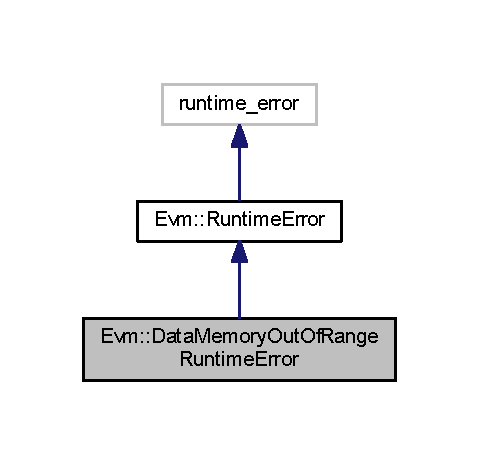
\includegraphics[width=230pt]{struct_evm_1_1_data_memory_out_of_range_runtime_error__inherit__graph}
\end{center}
\end{figure}


Collaboration diagram for Evm\+:\+:Data\+Memory\+Out\+Of\+Range\+Runtime\+Error\+:
\nopagebreak
\begin{figure}[H]
\begin{center}
\leavevmode
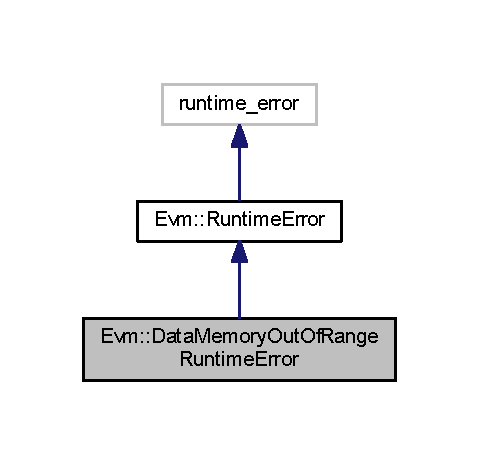
\includegraphics[width=230pt]{struct_evm_1_1_data_memory_out_of_range_runtime_error__coll__graph}
\end{center}
\end{figure}
\subsection*{Public Member Functions}
\begin{DoxyCompactItemize}
\item 
\mbox{\Hypertarget{struct_evm_1_1_data_memory_out_of_range_runtime_error_a7b19bd3e8e2efa7658f08ecf8387a4e3}\label{struct_evm_1_1_data_memory_out_of_range_runtime_error_a7b19bd3e8e2efa7658f08ecf8387a4e3}} 
{\bfseries Data\+Memory\+Out\+Of\+Range\+Runtime\+Error} (string \&msg)
\end{DoxyCompactItemize}


The documentation for this struct was generated from the following file\+:\begin{DoxyCompactItemize}
\item 
Evm/Runtime\+Error.\+h\end{DoxyCompactItemize}

\hypertarget{struct_evm_1_1_file_1_1_evm_file}{}\section{Evm\+:\+:File\+:\+:Evm\+File Struct Reference}
\label{struct_evm_1_1_file_1_1_evm_file}\index{Evm\+::\+File\+::\+Evm\+File@{Evm\+::\+File\+::\+Evm\+File}}


Collaboration diagram for Evm\+:\+:File\+:\+:Evm\+File\+:
\nopagebreak
\begin{figure}[H]
\begin{center}
\leavevmode
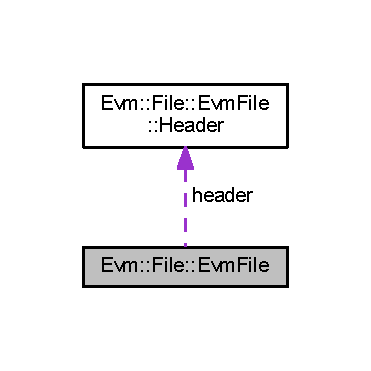
\includegraphics[width=178pt]{struct_evm_1_1_file_1_1_evm_file__coll__graph}
\end{center}
\end{figure}
\subsection*{Classes}
\begin{DoxyCompactItemize}
\item 
struct \mbox{\hyperlink{struct_evm_1_1_file_1_1_evm_file_1_1_header}{Header}}
\end{DoxyCompactItemize}
\subsection*{Public Attributes}
\begin{DoxyCompactItemize}
\item 
\mbox{\Hypertarget{struct_evm_1_1_file_1_1_evm_file_a72271701da24a49b5168e5c77214b918}\label{struct_evm_1_1_file_1_1_evm_file_a72271701da24a49b5168e5c77214b918}} 
\mbox{\hyperlink{struct_evm_1_1_file_1_1_evm_file_1_1_header}{Header}} {\bfseries header}
\item 
\mbox{\Hypertarget{struct_evm_1_1_file_1_1_evm_file_a7a7ce7b3e4b2a4df628afd399f1d0c8d}\label{struct_evm_1_1_file_1_1_evm_file_a7a7ce7b3e4b2a4df628afd399f1d0c8d}} 
Bytes {\bfseries payload}
\item 
\mbox{\Hypertarget{struct_evm_1_1_file_1_1_evm_file_ac5104283184f117667e68b82019739d5}\label{struct_evm_1_1_file_1_1_evm_file_ac5104283184f117667e68b82019739d5}} 
size\+\_\+t {\bfseries file\+Size}
\end{DoxyCompactItemize}


The documentation for this struct was generated from the following file\+:\begin{DoxyCompactItemize}
\item 
Evm/Evm\+File.\+h\end{DoxyCompactItemize}

\hypertarget{struct_evm_1_1_evm_file_parse_runtime_error}{}\section{Evm\+:\+:Evm\+File\+Parse\+Runtime\+Error Struct Reference}
\label{struct_evm_1_1_evm_file_parse_runtime_error}\index{Evm\+::\+Evm\+File\+Parse\+Runtime\+Error@{Evm\+::\+Evm\+File\+Parse\+Runtime\+Error}}


Inheritance diagram for Evm\+:\+:Evm\+File\+Parse\+Runtime\+Error\+:
\nopagebreak
\begin{figure}[H]
\begin{center}
\leavevmode
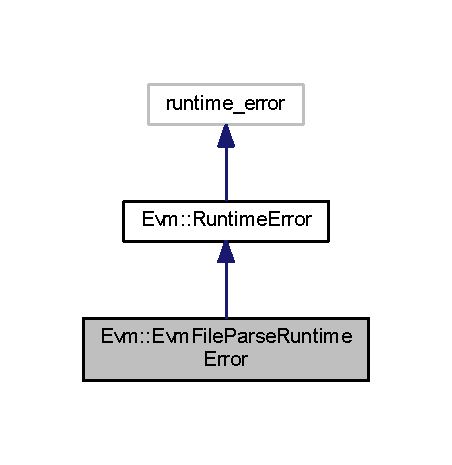
\includegraphics[width=217pt]{struct_evm_1_1_evm_file_parse_runtime_error__inherit__graph}
\end{center}
\end{figure}


Collaboration diagram for Evm\+:\+:Evm\+File\+Parse\+Runtime\+Error\+:
\nopagebreak
\begin{figure}[H]
\begin{center}
\leavevmode
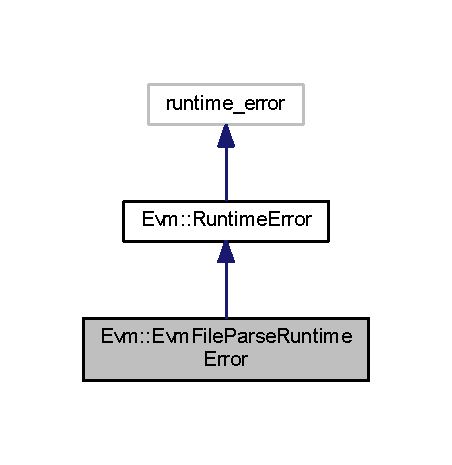
\includegraphics[width=217pt]{struct_evm_1_1_evm_file_parse_runtime_error__coll__graph}
\end{center}
\end{figure}
\subsection*{Public Member Functions}
\begin{DoxyCompactItemize}
\item 
\mbox{\Hypertarget{struct_evm_1_1_evm_file_parse_runtime_error_afda9b72b748cd4ac4c6becb0659b2f46}\label{struct_evm_1_1_evm_file_parse_runtime_error_afda9b72b748cd4ac4c6becb0659b2f46}} 
{\bfseries Evm\+File\+Parse\+Runtime\+Error} (const string \&msg)
\end{DoxyCompactItemize}


The documentation for this struct was generated from the following file\+:\begin{DoxyCompactItemize}
\item 
Evm/Runtime\+Error.\+h\end{DoxyCompactItemize}

\hypertarget{struct_evm_1_1_file_1_1_evm_file_1_1_header}{}\section{Evm\+:\+:File\+:\+:Evm\+File\+:\+:Header Struct Reference}
\label{struct_evm_1_1_file_1_1_evm_file_1_1_header}\index{Evm\+::\+File\+::\+Evm\+File\+::\+Header@{Evm\+::\+File\+::\+Evm\+File\+::\+Header}}
\subsection*{Public Attributes}
\begin{DoxyCompactItemize}
\item 
\mbox{\Hypertarget{struct_evm_1_1_file_1_1_evm_file_1_1_header_a1626b86e5361c1ef9d6a2908a2671067}\label{struct_evm_1_1_file_1_1_evm_file_1_1_header_a1626b86e5361c1ef9d6a2908a2671067}} 
char {\bfseries magic} \mbox{[}8\mbox{]}
\item 
\mbox{\Hypertarget{struct_evm_1_1_file_1_1_evm_file_1_1_header_aa065e8a05b184f006f57522ff46b442a}\label{struct_evm_1_1_file_1_1_evm_file_1_1_header_aa065e8a05b184f006f57522ff46b442a}} 
uint32\+\_\+t {\bfseries code\+Size}
\item 
\mbox{\Hypertarget{struct_evm_1_1_file_1_1_evm_file_1_1_header_a34491776d9893594f1f52d3a4f644db9}\label{struct_evm_1_1_file_1_1_evm_file_1_1_header_a34491776d9893594f1f52d3a4f644db9}} 
uint32\+\_\+t {\bfseries data\+Size}
\item 
\mbox{\Hypertarget{struct_evm_1_1_file_1_1_evm_file_1_1_header_aba896e5d58983d7623e5e822ca619680}\label{struct_evm_1_1_file_1_1_evm_file_1_1_header_aba896e5d58983d7623e5e822ca619680}} 
uint32\+\_\+t {\bfseries initial\+Data\+Size}
\end{DoxyCompactItemize}


The documentation for this struct was generated from the following file\+:\begin{DoxyCompactItemize}
\item 
Evm/Evm\+File.\+h\end{DoxyCompactItemize}

\hypertarget{struct_evm_1_1_operation_1_1_hlt_operation}{}\section{Evm\+:\+:Operation\+:\+:Hlt\+Operation Struct Reference}
\label{struct_evm_1_1_operation_1_1_hlt_operation}\index{Evm\+::\+Operation\+::\+Hlt\+Operation@{Evm\+::\+Operation\+::\+Hlt\+Operation}}


hlt operation  




{\ttfamily \#include $<$Operation.\+h$>$}



Inheritance diagram for Evm\+:\+:Operation\+:\+:Hlt\+Operation\+:
\nopagebreak
\begin{figure}[H]
\begin{center}
\leavevmode
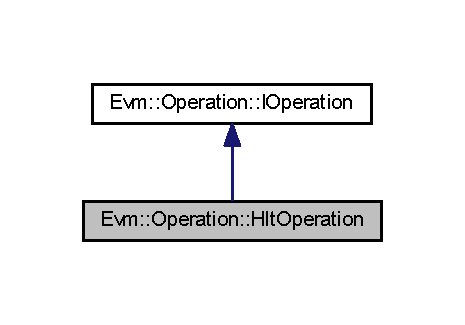
\includegraphics[width=223pt]{struct_evm_1_1_operation_1_1_hlt_operation__inherit__graph}
\end{center}
\end{figure}


Collaboration diagram for Evm\+:\+:Operation\+:\+:Hlt\+Operation\+:
\nopagebreak
\begin{figure}[H]
\begin{center}
\leavevmode
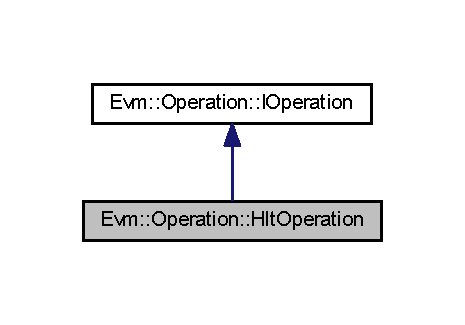
\includegraphics[width=223pt]{struct_evm_1_1_operation_1_1_hlt_operation__coll__graph}
\end{center}
\end{figure}
\subsection*{Public Member Functions}
\begin{DoxyCompactItemize}
\item 
virtual void \mbox{\hyperlink{struct_evm_1_1_operation_1_1_hlt_operation_a9b3fa2b5d0725a4ba842ce6a18c6b02d}{execute}} (\mbox{\hyperlink{struct_evm_1_1_thread_context}{Thread\+Context}} \&thread) override
\begin{DoxyCompactList}\small\item\em Execution of the instruction. \end{DoxyCompactList}\item 
\mbox{\hyperlink{struct_evm_1_1_operation_1_1_hlt_operation_a65e98ee1b1679e12c1d1dd000ebfe937}{I\+Operation}} (string \&opcode)
\begin{DoxyCompactList}\small\item\em Constructor. \end{DoxyCompactList}\end{DoxyCompactItemize}
\subsection*{Additional Inherited Members}


\subsection{Detailed Description}
hlt operation 

hlt; End current thread. If initial thread is ended, end whole program. 

\subsection{Member Function Documentation}
\mbox{\Hypertarget{struct_evm_1_1_operation_1_1_hlt_operation_a9b3fa2b5d0725a4ba842ce6a18c6b02d}\label{struct_evm_1_1_operation_1_1_hlt_operation_a9b3fa2b5d0725a4ba842ce6a18c6b02d}} 
\index{Evm\+::\+Operation\+::\+Hlt\+Operation@{Evm\+::\+Operation\+::\+Hlt\+Operation}!execute@{execute}}
\index{execute@{execute}!Evm\+::\+Operation\+::\+Hlt\+Operation@{Evm\+::\+Operation\+::\+Hlt\+Operation}}
\subsubsection{\texorpdfstring{execute()}{execute()}}
{\footnotesize\ttfamily void Evm\+::\+Operation\+::\+Hlt\+Operation\+::execute (\begin{DoxyParamCaption}\item[{\mbox{\hyperlink{struct_evm_1_1_thread_context}{Thread\+Context}} \&}]{thread }\end{DoxyParamCaption})\hspace{0.3cm}{\ttfamily [override]}, {\ttfamily [virtual]}}



Execution of the instruction. 

May by call by an application to execute the operation. The execution requires to be awared of thread context within the operation is executed. 
\begin{DoxyParams}{Parameters}
{\em thread} & Context of \mbox{\hyperlink{namespace_evm}{Evm}} thread \\
\hline
\end{DoxyParams}


Implements \mbox{\hyperlink{struct_evm_1_1_operation_1_1_i_operation_a7285631335da103423c01471dedeb1d7}{Evm\+::\+Operation\+::\+I\+Operation}}.

\mbox{\Hypertarget{struct_evm_1_1_operation_1_1_hlt_operation_a65e98ee1b1679e12c1d1dd000ebfe937}\label{struct_evm_1_1_operation_1_1_hlt_operation_a65e98ee1b1679e12c1d1dd000ebfe937}} 
\index{Evm\+::\+Operation\+::\+Hlt\+Operation@{Evm\+::\+Operation\+::\+Hlt\+Operation}!I\+Operation@{I\+Operation}}
\index{I\+Operation@{I\+Operation}!Evm\+::\+Operation\+::\+Hlt\+Operation@{Evm\+::\+Operation\+::\+Hlt\+Operation}}
\subsubsection{\texorpdfstring{I\+Operation()}{IOperation()}}
{\footnotesize\ttfamily Evm\+::\+Operation\+::\+I\+Operation\+::\+I\+Operation\hspace{0.3cm}{\ttfamily [inline]}}



Constructor. 


\begin{DoxyParams}{Parameters}
{\em opcode} & Printable label of the instruction \\
\hline
\end{DoxyParams}


The documentation for this struct was generated from the following files\+:\begin{DoxyCompactItemize}
\item 
Evm/Operation.\+h\item 
Evm/\mbox{\hyperlink{_operation_8cpp}{Operation.\+cpp}}\end{DoxyCompactItemize}

\hypertarget{struct_evm_1_1_argument_1_1_i_argument}{}\section{Evm\+:\+:Argument\+:\+:I\+Argument Struct Reference}
\label{struct_evm_1_1_argument_1_1_i_argument}\index{Evm\+::\+Argument\+::\+I\+Argument@{Evm\+::\+Argument\+::\+I\+Argument}}


Inheritance diagram for Evm\+:\+:Argument\+:\+:I\+Argument\+:
\nopagebreak
\begin{figure}[H]
\begin{center}
\leavevmode
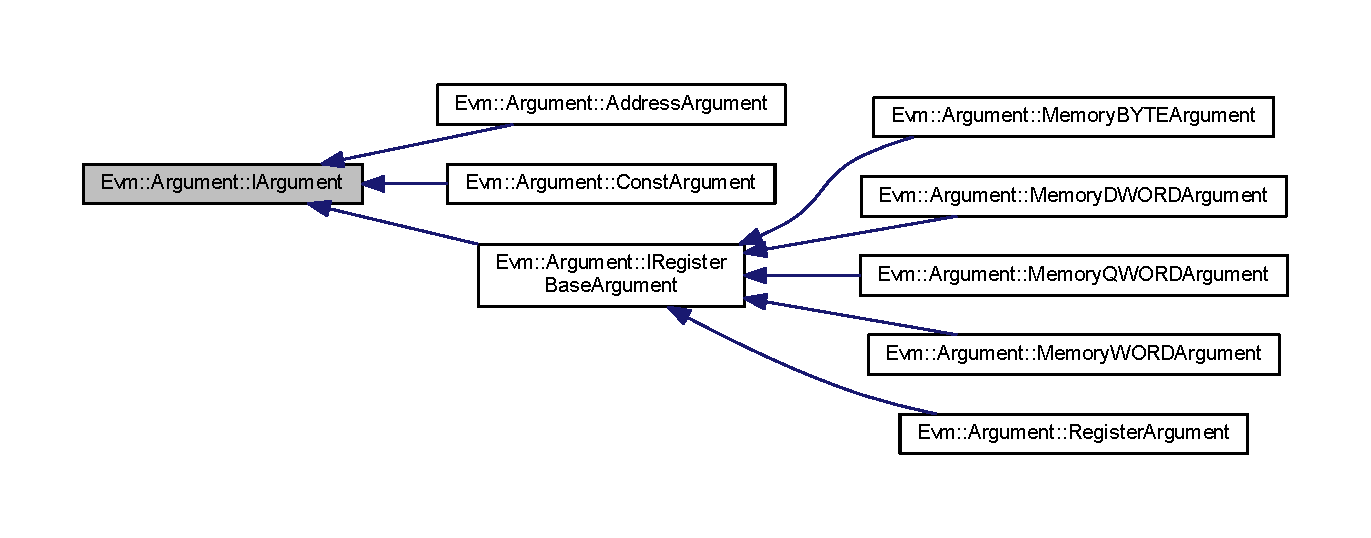
\includegraphics[width=350pt]{struct_evm_1_1_argument_1_1_i_argument__inherit__graph}
\end{center}
\end{figure}
\subsection*{Public Member Functions}
\begin{DoxyCompactItemize}
\item 
\mbox{\Hypertarget{struct_evm_1_1_argument_1_1_i_argument_a46a050eab0061cce199ca390bb91ed0a}\label{struct_evm_1_1_argument_1_1_i_argument_a46a050eab0061cce199ca390bb91ed0a}} 
virtual \mbox{\hyperlink{struct_evm_1_1_argument_1_1_i_argument_a46a050eab0061cce199ca390bb91ed0a}{$\sim$\+I\+Argument}} ()=default
\begin{DoxyCompactList}\small\item\em Virtual destructor. \end{DoxyCompactList}\item 
virtual uint64\+\_\+t \mbox{\hyperlink{struct_evm_1_1_argument_1_1_i_argument_af01db10f34498344831877847c2fc038}{get\+Value}} (\mbox{\hyperlink{struct_evm_1_1_thread_context}{Thread\+Context}} \&thread) const =0
\begin{DoxyCompactList}\small\item\em Get value. \end{DoxyCompactList}\item 
virtual void \mbox{\hyperlink{struct_evm_1_1_argument_1_1_i_argument_a24e4c76f2750e664e3895d2ff4b9146d}{set\+Value}} (\mbox{\hyperlink{struct_evm_1_1_thread_context}{Thread\+Context}} \&thread, uint64\+\_\+t value)=0
\begin{DoxyCompactList}\small\item\em Set value. \end{DoxyCompactList}\item 
virtual string \mbox{\hyperlink{struct_evm_1_1_argument_1_1_i_argument_a35bdae816e89f6f9fc393b6e03c5e521}{label}} () const =0
\begin{DoxyCompactList}\small\item\em Get printable representation of the argument. \end{DoxyCompactList}\item 
virtual string \mbox{\hyperlink{struct_evm_1_1_argument_1_1_i_argument_afcab2d2a1515518a111881a635c83da3}{print\+Value}} (\mbox{\hyperlink{struct_evm_1_1_thread_context}{Thread\+Context}} \&thread) const =0
\begin{DoxyCompactList}\small\item\em Get printable value of the parameter. \end{DoxyCompactList}\end{DoxyCompactItemize}


\subsection{Member Function Documentation}
\mbox{\Hypertarget{struct_evm_1_1_argument_1_1_i_argument_af01db10f34498344831877847c2fc038}\label{struct_evm_1_1_argument_1_1_i_argument_af01db10f34498344831877847c2fc038}} 
\index{Evm\+::\+Argument\+::\+I\+Argument@{Evm\+::\+Argument\+::\+I\+Argument}!get\+Value@{get\+Value}}
\index{get\+Value@{get\+Value}!Evm\+::\+Argument\+::\+I\+Argument@{Evm\+::\+Argument\+::\+I\+Argument}}
\subsubsection{\texorpdfstring{get\+Value()}{getValue()}}
{\footnotesize\ttfamily virtual uint64\+\_\+t Evm\+::\+Argument\+::\+I\+Argument\+::get\+Value (\begin{DoxyParamCaption}\item[{\mbox{\hyperlink{struct_evm_1_1_thread_context}{Thread\+Context}} \&}]{thread }\end{DoxyParamCaption}) const\hspace{0.3cm}{\ttfamily [pure virtual]}}



Get value. 

Return value of the argument 
\begin{DoxyParams}{Parameters}
{\em thread} & Thread context within this argument is used \\
\hline
\end{DoxyParams}
\begin{DoxyReturn}{Returns}
Value of the parameter 
\end{DoxyReturn}


Implemented in \mbox{\hyperlink{struct_evm_1_1_argument_1_1_address_argument_a8dfdf1626e06e7c72af39ca3f09ecec7}{Evm\+::\+Argument\+::\+Address\+Argument}}, \mbox{\hyperlink{struct_evm_1_1_argument_1_1_const_argument_abd4e5bb5fdad5eb9bd76436ea9c6836c}{Evm\+::\+Argument\+::\+Const\+Argument}}, \mbox{\hyperlink{struct_evm_1_1_argument_1_1_memory_q_w_o_r_d_argument_a07ee2f720366e41d8509f3c5aef8a46a}{Evm\+::\+Argument\+::\+Memory\+Q\+W\+O\+R\+D\+Argument}}, \mbox{\hyperlink{struct_evm_1_1_argument_1_1_memory_d_w_o_r_d_argument_a2236851a43925f9c93db6d107bc5986e}{Evm\+::\+Argument\+::\+Memory\+D\+W\+O\+R\+D\+Argument}}, \mbox{\hyperlink{struct_evm_1_1_argument_1_1_memory_w_o_r_d_argument_a689f534d26558b10f9d10ae80e221dee}{Evm\+::\+Argument\+::\+Memory\+W\+O\+R\+D\+Argument}}, \mbox{\hyperlink{struct_evm_1_1_argument_1_1_memory_b_y_t_e_argument_af038f3d7e425ef70f5688bda45eb8d31}{Evm\+::\+Argument\+::\+Memory\+B\+Y\+T\+E\+Argument}}, and \mbox{\hyperlink{struct_evm_1_1_argument_1_1_register_argument_aa2bb3ec054c1370ccde12b283f9887b1}{Evm\+::\+Argument\+::\+Register\+Argument}}.

\mbox{\Hypertarget{struct_evm_1_1_argument_1_1_i_argument_a35bdae816e89f6f9fc393b6e03c5e521}\label{struct_evm_1_1_argument_1_1_i_argument_a35bdae816e89f6f9fc393b6e03c5e521}} 
\index{Evm\+::\+Argument\+::\+I\+Argument@{Evm\+::\+Argument\+::\+I\+Argument}!label@{label}}
\index{label@{label}!Evm\+::\+Argument\+::\+I\+Argument@{Evm\+::\+Argument\+::\+I\+Argument}}
\subsubsection{\texorpdfstring{label()}{label()}}
{\footnotesize\ttfamily virtual string Evm\+::\+Argument\+::\+I\+Argument\+::label (\begin{DoxyParamCaption}{ }\end{DoxyParamCaption}) const\hspace{0.3cm}{\ttfamily [pure virtual]}}



Get printable representation of the argument. 

\begin{DoxyReturn}{Returns}
string with argument label 
\end{DoxyReturn}


Implemented in \mbox{\hyperlink{struct_evm_1_1_argument_1_1_address_argument_a4a8ca0f63e6139140f924c2cab9b3d40}{Evm\+::\+Argument\+::\+Address\+Argument}}, \mbox{\hyperlink{struct_evm_1_1_argument_1_1_const_argument_a90801800ff37e785e946f077f1c486f6}{Evm\+::\+Argument\+::\+Const\+Argument}}, \mbox{\hyperlink{struct_evm_1_1_argument_1_1_memory_q_w_o_r_d_argument_adb47000f058eca32e797c63857b4a558}{Evm\+::\+Argument\+::\+Memory\+Q\+W\+O\+R\+D\+Argument}}, \mbox{\hyperlink{struct_evm_1_1_argument_1_1_memory_d_w_o_r_d_argument_aa65e3072de44a5261193fdcfa2babc11}{Evm\+::\+Argument\+::\+Memory\+D\+W\+O\+R\+D\+Argument}}, \mbox{\hyperlink{struct_evm_1_1_argument_1_1_memory_w_o_r_d_argument_a3a719074885eb9d1329e75a2b888bd47}{Evm\+::\+Argument\+::\+Memory\+W\+O\+R\+D\+Argument}}, \mbox{\hyperlink{struct_evm_1_1_argument_1_1_memory_b_y_t_e_argument_afbe889873f7f6c825d9554e2029294b3}{Evm\+::\+Argument\+::\+Memory\+B\+Y\+T\+E\+Argument}}, and \mbox{\hyperlink{struct_evm_1_1_argument_1_1_register_argument_ab464babd0865a84e76265843c355220b}{Evm\+::\+Argument\+::\+Register\+Argument}}.

\mbox{\Hypertarget{struct_evm_1_1_argument_1_1_i_argument_afcab2d2a1515518a111881a635c83da3}\label{struct_evm_1_1_argument_1_1_i_argument_afcab2d2a1515518a111881a635c83da3}} 
\index{Evm\+::\+Argument\+::\+I\+Argument@{Evm\+::\+Argument\+::\+I\+Argument}!print\+Value@{print\+Value}}
\index{print\+Value@{print\+Value}!Evm\+::\+Argument\+::\+I\+Argument@{Evm\+::\+Argument\+::\+I\+Argument}}
\subsubsection{\texorpdfstring{print\+Value()}{printValue()}}
{\footnotesize\ttfamily virtual string Evm\+::\+Argument\+::\+I\+Argument\+::print\+Value (\begin{DoxyParamCaption}\item[{\mbox{\hyperlink{struct_evm_1_1_thread_context}{Thread\+Context}} \&}]{thread }\end{DoxyParamCaption}) const\hspace{0.3cm}{\ttfamily [pure virtual]}}



Get printable value of the parameter. 


\begin{DoxyParams}{Parameters}
{\em thread} & Thread context within this argument is used \\
\hline
\end{DoxyParams}
\begin{DoxyReturn}{Returns}
string with argument value 
\end{DoxyReturn}


Implemented in \mbox{\hyperlink{struct_evm_1_1_argument_1_1_address_argument_afaefa598d24c588a0047df1b88033bbd}{Evm\+::\+Argument\+::\+Address\+Argument}}, \mbox{\hyperlink{struct_evm_1_1_argument_1_1_const_argument_a5741f701088fadebf19b733c6973898b}{Evm\+::\+Argument\+::\+Const\+Argument}}, \mbox{\hyperlink{struct_evm_1_1_argument_1_1_memory_q_w_o_r_d_argument_a428099eec7efa97b28a07f9b4d1a257b}{Evm\+::\+Argument\+::\+Memory\+Q\+W\+O\+R\+D\+Argument}}, \mbox{\hyperlink{struct_evm_1_1_argument_1_1_memory_d_w_o_r_d_argument_adea7b11736aa7af73ad702e6aaf6e464}{Evm\+::\+Argument\+::\+Memory\+D\+W\+O\+R\+D\+Argument}}, \mbox{\hyperlink{struct_evm_1_1_argument_1_1_memory_w_o_r_d_argument_ac8c383d86bde6ef724583560bd0436e0}{Evm\+::\+Argument\+::\+Memory\+W\+O\+R\+D\+Argument}}, \mbox{\hyperlink{struct_evm_1_1_argument_1_1_memory_b_y_t_e_argument_a7fbed3cafe6784094617c522a2c91412}{Evm\+::\+Argument\+::\+Memory\+B\+Y\+T\+E\+Argument}}, and \mbox{\hyperlink{struct_evm_1_1_argument_1_1_register_argument_a68e1690a92a7e7844fd89cc9b2dd3a6c}{Evm\+::\+Argument\+::\+Register\+Argument}}.

\mbox{\Hypertarget{struct_evm_1_1_argument_1_1_i_argument_a24e4c76f2750e664e3895d2ff4b9146d}\label{struct_evm_1_1_argument_1_1_i_argument_a24e4c76f2750e664e3895d2ff4b9146d}} 
\index{Evm\+::\+Argument\+::\+I\+Argument@{Evm\+::\+Argument\+::\+I\+Argument}!set\+Value@{set\+Value}}
\index{set\+Value@{set\+Value}!Evm\+::\+Argument\+::\+I\+Argument@{Evm\+::\+Argument\+::\+I\+Argument}}
\subsubsection{\texorpdfstring{set\+Value()}{setValue()}}
{\footnotesize\ttfamily virtual void Evm\+::\+Argument\+::\+I\+Argument\+::set\+Value (\begin{DoxyParamCaption}\item[{\mbox{\hyperlink{struct_evm_1_1_thread_context}{Thread\+Context}} \&}]{thread,  }\item[{uint64\+\_\+t}]{value }\end{DoxyParamCaption})\hspace{0.3cm}{\ttfamily [pure virtual]}}



Set value. 

Set value of the argument. \begin{DoxyWarning}{Warning}
For read-\/only arguments this throws an exception 
\end{DoxyWarning}

\begin{DoxyParams}{Parameters}
{\em thread} & Thread context within this argument is used \\
\hline
{\em value} & New value of the parameter \\
\hline
\end{DoxyParams}


Implemented in \mbox{\hyperlink{struct_evm_1_1_argument_1_1_address_argument_a2fa90885150424134b181ff01704e798}{Evm\+::\+Argument\+::\+Address\+Argument}}, \mbox{\hyperlink{struct_evm_1_1_argument_1_1_const_argument_ab456fa9175551b4c04815ccd65c76bd2}{Evm\+::\+Argument\+::\+Const\+Argument}}, \mbox{\hyperlink{struct_evm_1_1_argument_1_1_memory_q_w_o_r_d_argument_aff2a33f879d440a90c93a7635c5d705a}{Evm\+::\+Argument\+::\+Memory\+Q\+W\+O\+R\+D\+Argument}}, \mbox{\hyperlink{struct_evm_1_1_argument_1_1_memory_d_w_o_r_d_argument_ad1b0d692889006c0db43740f099d8689}{Evm\+::\+Argument\+::\+Memory\+D\+W\+O\+R\+D\+Argument}}, \mbox{\hyperlink{struct_evm_1_1_argument_1_1_memory_w_o_r_d_argument_a9572abaa123939edd7c724074ac3b7ec}{Evm\+::\+Argument\+::\+Memory\+W\+O\+R\+D\+Argument}}, \mbox{\hyperlink{struct_evm_1_1_argument_1_1_memory_b_y_t_e_argument_a6da25d3c59f1676c39ac8f0f0f211863}{Evm\+::\+Argument\+::\+Memory\+B\+Y\+T\+E\+Argument}}, and \mbox{\hyperlink{struct_evm_1_1_argument_1_1_register_argument_afc97b81c554d6f77c9736178c54816cc}{Evm\+::\+Argument\+::\+Register\+Argument}}.



The documentation for this struct was generated from the following file\+:\begin{DoxyCompactItemize}
\item 
Evm/\mbox{\hyperlink{_argument_8h}{Argument.\+h}}\end{DoxyCompactItemize}

\hypertarget{struct_evm_1_1_input_file_runtime_error}{}\section{Evm\+:\+:Input\+File\+Runtime\+Error Struct Reference}
\label{struct_evm_1_1_input_file_runtime_error}\index{Evm\+::\+Input\+File\+Runtime\+Error@{Evm\+::\+Input\+File\+Runtime\+Error}}


Inheritance diagram for Evm\+:\+:Input\+File\+Runtime\+Error\+:
\nopagebreak
\begin{figure}[H]
\begin{center}
\leavevmode
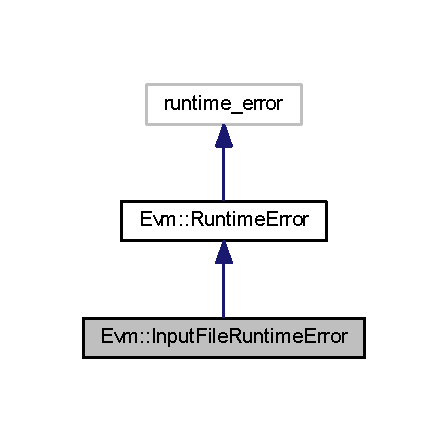
\includegraphics[width=215pt]{struct_evm_1_1_input_file_runtime_error__inherit__graph}
\end{center}
\end{figure}


Collaboration diagram for Evm\+:\+:Input\+File\+Runtime\+Error\+:
\nopagebreak
\begin{figure}[H]
\begin{center}
\leavevmode
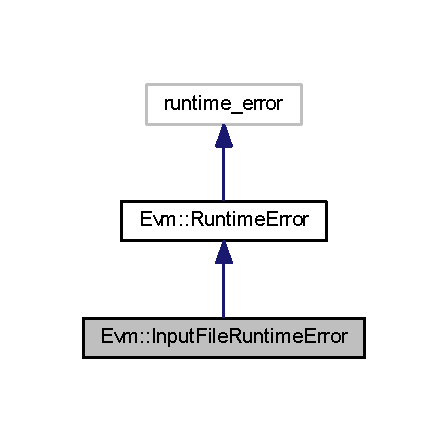
\includegraphics[width=215pt]{struct_evm_1_1_input_file_runtime_error__coll__graph}
\end{center}
\end{figure}
\subsection*{Public Member Functions}
\begin{DoxyCompactItemize}
\item 
\mbox{\Hypertarget{struct_evm_1_1_input_file_runtime_error_a082b779e70ab0d60fa26079884509c10}\label{struct_evm_1_1_input_file_runtime_error_a082b779e70ab0d60fa26079884509c10}} 
{\bfseries Input\+File\+Runtime\+Error} (const string \&filename, const string \&msg)
\item 
\mbox{\Hypertarget{struct_evm_1_1_input_file_runtime_error_a2b41c85cb364913cb5f0a47bcd273cf3}\label{struct_evm_1_1_input_file_runtime_error_a2b41c85cb364913cb5f0a47bcd273cf3}} 
{\bfseries Input\+File\+Runtime\+Error} (const string \&msg)
\end{DoxyCompactItemize}


The documentation for this struct was generated from the following file\+:\begin{DoxyCompactItemize}
\item 
Evm/Runtime\+Error.\+h\end{DoxyCompactItemize}

\hypertarget{struct_evm_1_1_operation_1_1_i_operation}{}\section{Evm\+:\+:Operation\+:\+:I\+Operation Struct Reference}
\label{struct_evm_1_1_operation_1_1_i_operation}\index{Evm\+::\+Operation\+::\+I\+Operation@{Evm\+::\+Operation\+::\+I\+Operation}}


\mbox{\hyperlink{struct_evm_1_1_operation_1_1_i_operation}{I\+Operation}} interface. Abstraction of \mbox{\hyperlink{namespace_evm}{Evm}} instruction.  




{\ttfamily \#include $<$Operation.\+h$>$}



Inheritance diagram for Evm\+:\+:Operation\+:\+:I\+Operation\+:
\nopagebreak
\begin{figure}[H]
\begin{center}
\leavevmode
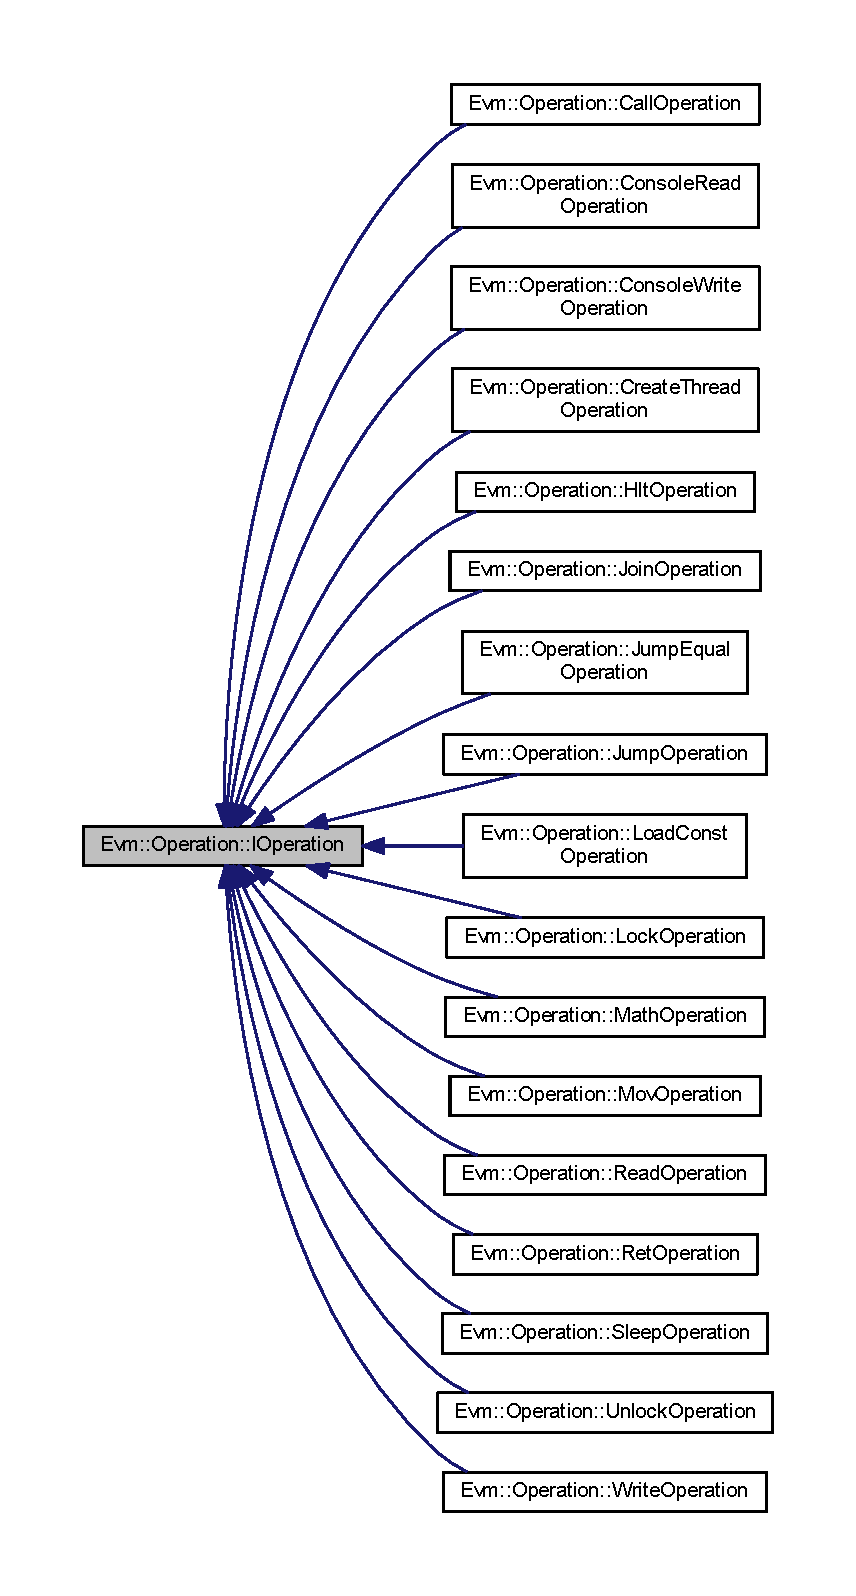
\includegraphics[height=550pt]{struct_evm_1_1_operation_1_1_i_operation__inherit__graph}
\end{center}
\end{figure}
\subsection*{Public Member Functions}
\begin{DoxyCompactItemize}
\item 
\mbox{\hyperlink{struct_evm_1_1_operation_1_1_i_operation_a65e98ee1b1679e12c1d1dd000ebfe937}{I\+Operation}} (string \&opcode)
\begin{DoxyCompactList}\small\item\em Constructor. \end{DoxyCompactList}\item 
\mbox{\Hypertarget{struct_evm_1_1_operation_1_1_i_operation_a8a06e5afa77ea47b23728c642e7c39df}\label{struct_evm_1_1_operation_1_1_i_operation_a8a06e5afa77ea47b23728c642e7c39df}} 
virtual \mbox{\hyperlink{struct_evm_1_1_operation_1_1_i_operation_a8a06e5afa77ea47b23728c642e7c39df}{$\sim$\+I\+Operation}} ()=default
\begin{DoxyCompactList}\small\item\em Virtual destructor. \end{DoxyCompactList}\item 
virtual void \mbox{\hyperlink{struct_evm_1_1_operation_1_1_i_operation_a7285631335da103423c01471dedeb1d7}{execute}} (\mbox{\hyperlink{struct_evm_1_1_thread_context}{Thread\+Context}} \&thread)=0
\begin{DoxyCompactList}\small\item\em Execution of the instruction. \end{DoxyCompactList}\item 
void \mbox{\hyperlink{struct_evm_1_1_operation_1_1_i_operation_a800d9e3986654525f7674d8a7e534fa8}{push\+Argument}} (Argument\+Ptr arg)
\begin{DoxyCompactList}\small\item\em Assign argument to the operation. \end{DoxyCompactList}\item 
string \mbox{\hyperlink{struct_evm_1_1_operation_1_1_i_operation_a32fef14914757a5c2312595810f363d1}{trace}} (\mbox{\hyperlink{struct_evm_1_1_thread_context}{Thread\+Context}} \&thread) const
\begin{DoxyCompactList}\small\item\em Print the operation. \end{DoxyCompactList}\end{DoxyCompactItemize}
\subsection*{Protected Attributes}
\begin{DoxyCompactItemize}
\item 
\mbox{\Hypertarget{struct_evm_1_1_operation_1_1_i_operation_a41039f84360a1ec0d86cf2eb92bafe97}\label{struct_evm_1_1_operation_1_1_i_operation_a41039f84360a1ec0d86cf2eb92bafe97}} 
string \mbox{\hyperlink{struct_evm_1_1_operation_1_1_i_operation_a41039f84360a1ec0d86cf2eb92bafe97}{\+\_\+opcode}}
\begin{DoxyCompactList}\small\item\em Printable opcode. \end{DoxyCompactList}\item 
\mbox{\Hypertarget{struct_evm_1_1_operation_1_1_i_operation_af12706aa091dddcd3f17e10797a232d7}\label{struct_evm_1_1_operation_1_1_i_operation_af12706aa091dddcd3f17e10797a232d7}} 
Argument\+List \mbox{\hyperlink{struct_evm_1_1_operation_1_1_i_operation_af12706aa091dddcd3f17e10797a232d7}{\+\_\+arg\+List}}
\begin{DoxyCompactList}\small\item\em Vector with arguments required by the instruction. \end{DoxyCompactList}\end{DoxyCompactItemize}
\subsection*{Friends}
\begin{DoxyCompactItemize}
\item 
ostream \& \mbox{\hyperlink{struct_evm_1_1_operation_1_1_i_operation_afed6ad5f16d9e581357397e96da68dae}{operator$<$$<$}} (ostream \&os, \mbox{\hyperlink{struct_evm_1_1_operation_1_1_i_operation}{I\+Operation}} \&op)
\begin{DoxyCompactList}\small\item\em Print the operation. \end{DoxyCompactList}\end{DoxyCompactItemize}


\subsection{Detailed Description}
\mbox{\hyperlink{struct_evm_1_1_operation_1_1_i_operation}{I\+Operation}} interface. Abstraction of \mbox{\hyperlink{namespace_evm}{Evm}} instruction. 

The class represents an \mbox{\hyperlink{namespace_evm}{Evm}} instruction. It provides three A\+PI methods, \mbox{\hyperlink{struct_evm_1_1_operation_1_1_i_operation_a7285631335da103423c01471dedeb1d7}{execute()}} -\/ to run the operaction, \mbox{\hyperlink{struct_evm_1_1_operation_1_1_i_operation_a32fef14914757a5c2312595810f363d1}{trace()}} -\/ to get printable representation and current values of arguemnts, and \mbox{\hyperlink{struct_evm_1_1_operation_1_1_i_operation_a800d9e3986654525f7674d8a7e534fa8}{push\+Argument()}} -\/ to assign arguments. 

\subsection{Constructor \& Destructor Documentation}
\mbox{\Hypertarget{struct_evm_1_1_operation_1_1_i_operation_a65e98ee1b1679e12c1d1dd000ebfe937}\label{struct_evm_1_1_operation_1_1_i_operation_a65e98ee1b1679e12c1d1dd000ebfe937}} 
\index{Evm\+::\+Operation\+::\+I\+Operation@{Evm\+::\+Operation\+::\+I\+Operation}!I\+Operation@{I\+Operation}}
\index{I\+Operation@{I\+Operation}!Evm\+::\+Operation\+::\+I\+Operation@{Evm\+::\+Operation\+::\+I\+Operation}}
\subsubsection{\texorpdfstring{I\+Operation()}{IOperation()}}
{\footnotesize\ttfamily Evm\+::\+Operation\+::\+I\+Operation\+::\+I\+Operation (\begin{DoxyParamCaption}\item[{string \&}]{opcode }\end{DoxyParamCaption})\hspace{0.3cm}{\ttfamily [inline]}}



Constructor. 


\begin{DoxyParams}{Parameters}
{\em opcode} & Printable label of the instruction \\
\hline
\end{DoxyParams}


\subsection{Member Function Documentation}
\mbox{\Hypertarget{struct_evm_1_1_operation_1_1_i_operation_a7285631335da103423c01471dedeb1d7}\label{struct_evm_1_1_operation_1_1_i_operation_a7285631335da103423c01471dedeb1d7}} 
\index{Evm\+::\+Operation\+::\+I\+Operation@{Evm\+::\+Operation\+::\+I\+Operation}!execute@{execute}}
\index{execute@{execute}!Evm\+::\+Operation\+::\+I\+Operation@{Evm\+::\+Operation\+::\+I\+Operation}}
\subsubsection{\texorpdfstring{execute()}{execute()}}
{\footnotesize\ttfamily virtual void Evm\+::\+Operation\+::\+I\+Operation\+::execute (\begin{DoxyParamCaption}\item[{\mbox{\hyperlink{struct_evm_1_1_thread_context}{Thread\+Context}} \&}]{thread }\end{DoxyParamCaption})\hspace{0.3cm}{\ttfamily [pure virtual]}}



Execution of the instruction. 

May by call by an application to execute the operation. The execution requires to be awared of thread context within the operation is executed. 
\begin{DoxyParams}{Parameters}
{\em thread} & Context of \mbox{\hyperlink{namespace_evm}{Evm}} thread \\
\hline
\end{DoxyParams}


Implemented in \mbox{\hyperlink{struct_evm_1_1_operation_1_1_read_operation_ab77f1e856a1b8a033cf4b8c0086f9222}{Evm\+::\+Operation\+::\+Read\+Operation}}, \mbox{\hyperlink{struct_evm_1_1_operation_1_1_write_operation_a66348759c19859b70c73cd1291c6efbb}{Evm\+::\+Operation\+::\+Write\+Operation}}, \mbox{\hyperlink{struct_evm_1_1_operation_1_1_unlock_operation_a012bb6185feb5186c5fe8c386068401a}{Evm\+::\+Operation\+::\+Unlock\+Operation}}, \mbox{\hyperlink{struct_evm_1_1_operation_1_1_lock_operation_a2ecf10dec9abb8203f56a8f119a97a7f}{Evm\+::\+Operation\+::\+Lock\+Operation}}, \mbox{\hyperlink{struct_evm_1_1_operation_1_1_sleep_operation_a12fd1e8e636dd9e9bc571c6769b6f926}{Evm\+::\+Operation\+::\+Sleep\+Operation}}, \mbox{\hyperlink{struct_evm_1_1_operation_1_1_join_operation_a55e6e5eb220d3ed0b659d085a7aa6df8}{Evm\+::\+Operation\+::\+Join\+Operation}}, \mbox{\hyperlink{struct_evm_1_1_operation_1_1_create_thread_operation_a5efc82f864a95f07bd4312522cd91c70}{Evm\+::\+Operation\+::\+Create\+Thread\+Operation}}, \mbox{\hyperlink{struct_evm_1_1_operation_1_1_jump_equal_operation_a5edc133dd24ca78cc59203ab3ba47763}{Evm\+::\+Operation\+::\+Jump\+Equal\+Operation}}, \mbox{\hyperlink{struct_evm_1_1_operation_1_1_ret_operation_a34e691c30765bc62ea4c19d2896750b1}{Evm\+::\+Operation\+::\+Ret\+Operation}}, \mbox{\hyperlink{struct_evm_1_1_operation_1_1_hlt_operation_a9b3fa2b5d0725a4ba842ce6a18c6b02d}{Evm\+::\+Operation\+::\+Hlt\+Operation}}, \mbox{\hyperlink{struct_evm_1_1_operation_1_1_jump_operation_a830ab356fc212ff9ace8b63b0d24dcb1}{Evm\+::\+Operation\+::\+Jump\+Operation}}, \mbox{\hyperlink{struct_evm_1_1_operation_1_1_call_operation_ace9fbeb98abf5de426629be6eec22fd2}{Evm\+::\+Operation\+::\+Call\+Operation}}, \mbox{\hyperlink{struct_evm_1_1_operation_1_1_console_read_operation_a7bd7cfc2022abbb7fc9b45a2c75083e0}{Evm\+::\+Operation\+::\+Console\+Read\+Operation}}, \mbox{\hyperlink{struct_evm_1_1_operation_1_1_console_write_operation_a5dc059cb2b6faacc3dd1b477eec645e1}{Evm\+::\+Operation\+::\+Console\+Write\+Operation}}, \mbox{\hyperlink{struct_evm_1_1_operation_1_1_load_const_operation_a434d2748c59ccf0e3d1977e87c110e15}{Evm\+::\+Operation\+::\+Load\+Const\+Operation}}, \mbox{\hyperlink{struct_evm_1_1_operation_1_1_mov_operation_ab14344cf9597038ad5e2dda9d1846136}{Evm\+::\+Operation\+::\+Mov\+Operation}}, and \mbox{\hyperlink{struct_evm_1_1_operation_1_1_math_operation_a5ffc66e4ff4e6f59b1cd2512aad54380}{Evm\+::\+Operation\+::\+Math\+Operation}}.

\mbox{\Hypertarget{struct_evm_1_1_operation_1_1_i_operation_a800d9e3986654525f7674d8a7e534fa8}\label{struct_evm_1_1_operation_1_1_i_operation_a800d9e3986654525f7674d8a7e534fa8}} 
\index{Evm\+::\+Operation\+::\+I\+Operation@{Evm\+::\+Operation\+::\+I\+Operation}!push\+Argument@{push\+Argument}}
\index{push\+Argument@{push\+Argument}!Evm\+::\+Operation\+::\+I\+Operation@{Evm\+::\+Operation\+::\+I\+Operation}}
\subsubsection{\texorpdfstring{push\+Argument()}{pushArgument()}}
{\footnotesize\ttfamily void Evm\+::\+Operation\+::\+I\+Operation\+::push\+Argument (\begin{DoxyParamCaption}\item[{Argument\+Ptr}]{arg }\end{DoxyParamCaption})\hspace{0.3cm}{\ttfamily [inline]}}



Assign argument to the operation. 

The function is used to assign an argument to the operation. \begin{DoxyNote}{Note}
Arguments order has to match arguemnt order in documentation 
\end{DoxyNote}

\begin{DoxyParams}{Parameters}
{\em arg} & An argument \\
\hline
\end{DoxyParams}
\mbox{\Hypertarget{struct_evm_1_1_operation_1_1_i_operation_a32fef14914757a5c2312595810f363d1}\label{struct_evm_1_1_operation_1_1_i_operation_a32fef14914757a5c2312595810f363d1}} 
\index{Evm\+::\+Operation\+::\+I\+Operation@{Evm\+::\+Operation\+::\+I\+Operation}!trace@{trace}}
\index{trace@{trace}!Evm\+::\+Operation\+::\+I\+Operation@{Evm\+::\+Operation\+::\+I\+Operation}}
\subsubsection{\texorpdfstring{trace()}{trace()}}
{\footnotesize\ttfamily string Evm\+::\+Operation\+::\+I\+Operation\+::trace (\begin{DoxyParamCaption}\item[{\mbox{\hyperlink{struct_evm_1_1_thread_context}{Thread\+Context}} \&}]{thread }\end{DoxyParamCaption}) const}



Print the operation. 

Return a strign with printable verson of the operation, arguments and values of the arguments before execution 
\begin{DoxyParams}{Parameters}
{\em thread} & Thread contex \\
\hline
\end{DoxyParams}
\begin{DoxyNote}{Note}
It is possible to print an operation with argument list without current values. In that case the thread contex is not required see $<$$<$ operator 
\end{DoxyNote}


\subsection{Friends And Related Function Documentation}
\mbox{\Hypertarget{struct_evm_1_1_operation_1_1_i_operation_afed6ad5f16d9e581357397e96da68dae}\label{struct_evm_1_1_operation_1_1_i_operation_afed6ad5f16d9e581357397e96da68dae}} 
\index{Evm\+::\+Operation\+::\+I\+Operation@{Evm\+::\+Operation\+::\+I\+Operation}!operator$<$$<$@{operator$<$$<$}}
\index{operator$<$$<$@{operator$<$$<$}!Evm\+::\+Operation\+::\+I\+Operation@{Evm\+::\+Operation\+::\+I\+Operation}}
\subsubsection{\texorpdfstring{operator$<$$<$}{operator<<}}
{\footnotesize\ttfamily ostream\& operator$<$$<$ (\begin{DoxyParamCaption}\item[{ostream \&}]{os,  }\item[{\mbox{\hyperlink{struct_evm_1_1_operation_1_1_i_operation}{I\+Operation}} \&}]{op }\end{DoxyParamCaption})\hspace{0.3cm}{\ttfamily [friend]}}



Print the operation. 

Stream output operator that prints the operation without runtime data 

The documentation for this struct was generated from the following files\+:\begin{DoxyCompactItemize}
\item 
Evm/Operation.\+h\item 
Evm/\mbox{\hyperlink{_operation_8cpp}{Operation.\+cpp}}\end{DoxyCompactItemize}

\hypertarget{struct_evm_1_1_operation_1_1_i_operation_factory}{}\section{Evm\+:\+:Operation\+:\+:I\+Operation\+Factory Struct Reference}
\label{struct_evm_1_1_operation_1_1_i_operation_factory}\index{Evm\+::\+Operation\+::\+I\+Operation\+Factory@{Evm\+::\+Operation\+::\+I\+Operation\+Factory}}


Inheritance diagram for Evm\+:\+:Operation\+:\+:I\+Operation\+Factory\+:
\nopagebreak
\begin{figure}[H]
\begin{center}
\leavevmode
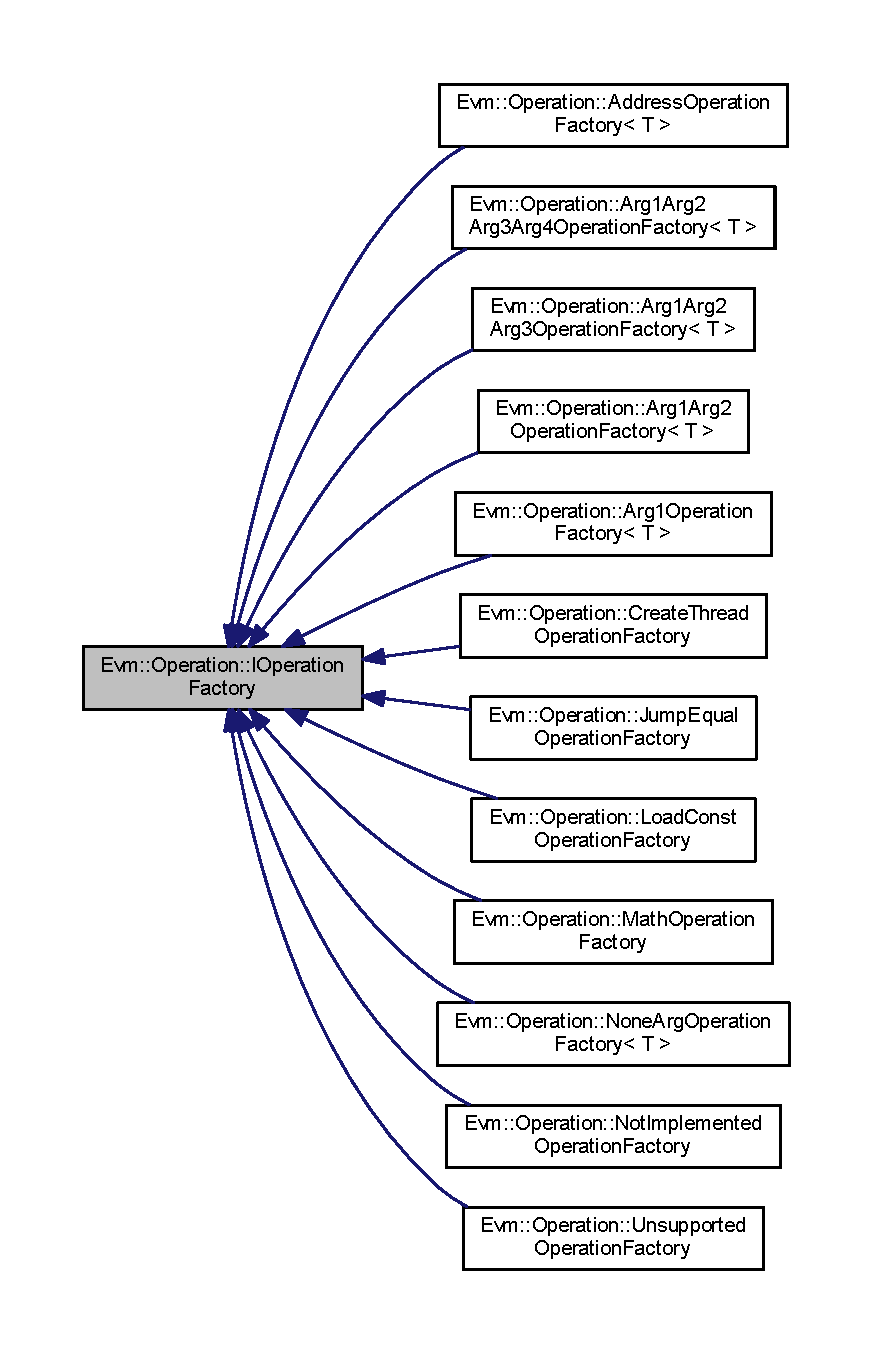
\includegraphics[width=350pt]{struct_evm_1_1_operation_1_1_i_operation_factory__inherit__graph}
\end{center}
\end{figure}


Collaboration diagram for Evm\+:\+:Operation\+:\+:I\+Operation\+Factory\+:
\nopagebreak
\begin{figure}[H]
\begin{center}
\leavevmode
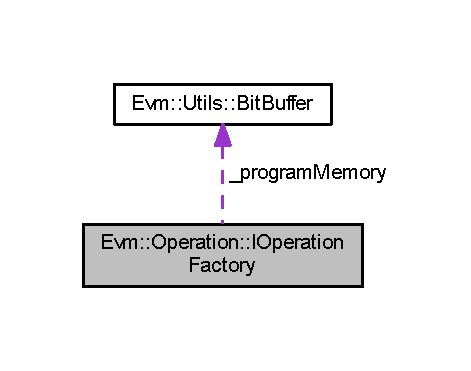
\includegraphics[width=226pt]{struct_evm_1_1_operation_1_1_i_operation_factory__coll__graph}
\end{center}
\end{figure}
\subsection*{Public Member Functions}
\begin{DoxyCompactItemize}
\item 
\mbox{\Hypertarget{struct_evm_1_1_operation_1_1_i_operation_factory_a7621b51ca2bc125b36be673486e33781}\label{struct_evm_1_1_operation_1_1_i_operation_factory_a7621b51ca2bc125b36be673486e33781}} 
{\bfseries I\+Operation\+Factory} (const string \&opcode, const \mbox{\hyperlink{struct_evm_1_1_utils_1_1_bit_buffer}{Utils\+::\+Bit\+Buffer}} \&program\+Memory)
\item 
\mbox{\Hypertarget{struct_evm_1_1_operation_1_1_i_operation_factory_a081d943adde12a09211a1e887029b471}\label{struct_evm_1_1_operation_1_1_i_operation_factory_a081d943adde12a09211a1e887029b471}} 
virtual Operation\+Ptr {\bfseries build} (uint32\+\_\+t \&offset)=0
\end{DoxyCompactItemize}
\subsection*{Protected Attributes}
\begin{DoxyCompactItemize}
\item 
\mbox{\Hypertarget{struct_evm_1_1_operation_1_1_i_operation_factory_a70bc63732326d70ca275a37f84c52e12}\label{struct_evm_1_1_operation_1_1_i_operation_factory_a70bc63732326d70ca275a37f84c52e12}} 
string {\bfseries \+\_\+opcode}
\item 
\mbox{\Hypertarget{struct_evm_1_1_operation_1_1_i_operation_factory_af921c76923ba9cc2483fb71ebab0fec1}\label{struct_evm_1_1_operation_1_1_i_operation_factory_af921c76923ba9cc2483fb71ebab0fec1}} 
const \mbox{\hyperlink{struct_evm_1_1_utils_1_1_bit_buffer}{Utils\+::\+Bit\+Buffer}} \& {\bfseries \+\_\+program\+Memory}
\end{DoxyCompactItemize}


The documentation for this struct was generated from the following file\+:\begin{DoxyCompactItemize}
\item 
Evm/Operation\+Factory.\+h\end{DoxyCompactItemize}

\hypertarget{struct_evm_1_1_argument_1_1_i_register_base_argument}{}\section{Evm\+:\+:Argument\+:\+:I\+Register\+Base\+Argument Struct Reference}
\label{struct_evm_1_1_argument_1_1_i_register_base_argument}\index{Evm\+::\+Argument\+::\+I\+Register\+Base\+Argument@{Evm\+::\+Argument\+::\+I\+Register\+Base\+Argument}}


Inheritance diagram for Evm\+:\+:Argument\+:\+:I\+Register\+Base\+Argument\+:
\nopagebreak
\begin{figure}[H]
\begin{center}
\leavevmode
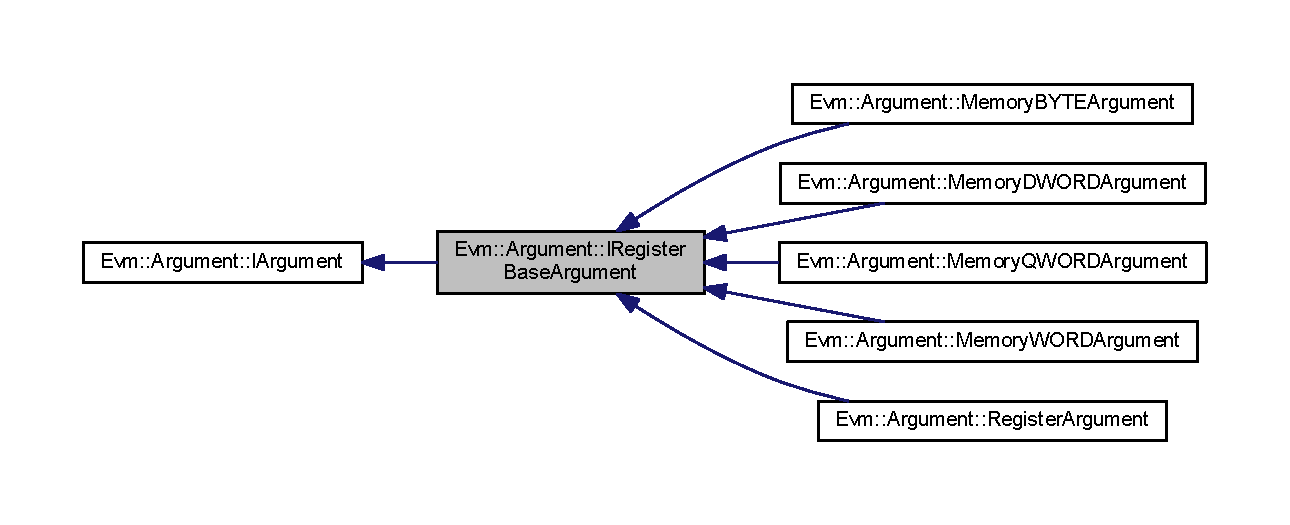
\includegraphics[width=350pt]{struct_evm_1_1_argument_1_1_i_register_base_argument__inherit__graph}
\end{center}
\end{figure}


Collaboration diagram for Evm\+:\+:Argument\+:\+:I\+Register\+Base\+Argument\+:
\nopagebreak
\begin{figure}[H]
\begin{center}
\leavevmode
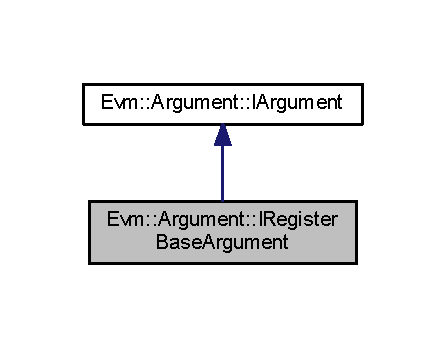
\includegraphics[width=214pt]{struct_evm_1_1_argument_1_1_i_register_base_argument__coll__graph}
\end{center}
\end{figure}
\subsection*{Public Member Functions}
\begin{DoxyCompactItemize}
\item 
\mbox{\Hypertarget{struct_evm_1_1_argument_1_1_i_register_base_argument_aa3dfe476b956a51bb26409c1d8763e21}\label{struct_evm_1_1_argument_1_1_i_register_base_argument_aa3dfe476b956a51bb26409c1d8763e21}} 
{\bfseries I\+Register\+Base\+Argument} (uint8\+\_\+t register\+Index)
\end{DoxyCompactItemize}
\subsection*{Protected Attributes}
\begin{DoxyCompactItemize}
\item 
\mbox{\Hypertarget{struct_evm_1_1_argument_1_1_i_register_base_argument_ab0692f6f7e062fe12d3bcaf70f722805}\label{struct_evm_1_1_argument_1_1_i_register_base_argument_ab0692f6f7e062fe12d3bcaf70f722805}} 
uint8\+\_\+t {\bfseries \+\_\+reg\+Index}
\end{DoxyCompactItemize}


The documentation for this struct was generated from the following file\+:\begin{DoxyCompactItemize}
\item 
Evm/\mbox{\hyperlink{_argument_8h}{Argument.\+h}}\end{DoxyCompactItemize}

\hypertarget{struct_evm_1_1_operation_1_1_join_operation}{}\section{Evm\+:\+:Operation\+:\+:Join\+Operation Struct Reference}
\label{struct_evm_1_1_operation_1_1_join_operation}\index{Evm\+::\+Operation\+::\+Join\+Operation@{Evm\+::\+Operation\+::\+Join\+Operation}}


join\+Thread operation  




{\ttfamily \#include $<$Operation.\+h$>$}



Inheritance diagram for Evm\+:\+:Operation\+:\+:Join\+Operation\+:
\nopagebreak
\begin{figure}[H]
\begin{center}
\leavevmode
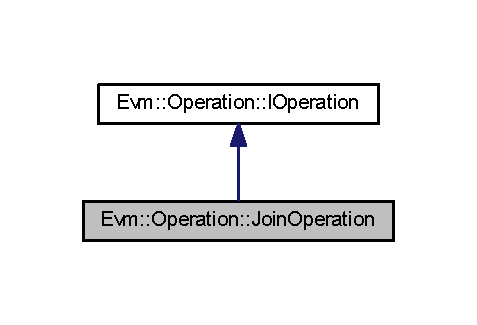
\includegraphics[width=229pt]{struct_evm_1_1_operation_1_1_join_operation__inherit__graph}
\end{center}
\end{figure}


Collaboration diagram for Evm\+:\+:Operation\+:\+:Join\+Operation\+:
\nopagebreak
\begin{figure}[H]
\begin{center}
\leavevmode
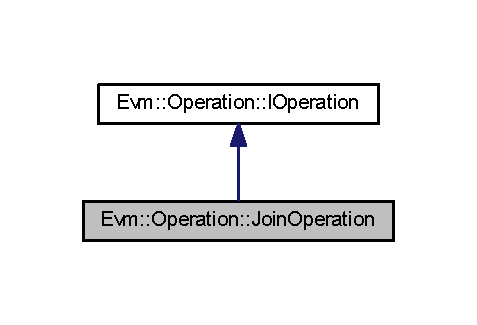
\includegraphics[width=229pt]{struct_evm_1_1_operation_1_1_join_operation__coll__graph}
\end{center}
\end{figure}
\subsection*{Public Member Functions}
\begin{DoxyCompactItemize}
\item 
virtual void \mbox{\hyperlink{struct_evm_1_1_operation_1_1_join_operation_a55e6e5eb220d3ed0b659d085a7aa6df8}{execute}} (\mbox{\hyperlink{struct_evm_1_1_thread_context}{Thread\+Context}} \&thread) override
\begin{DoxyCompactList}\small\item\em Execution of the instruction. \end{DoxyCompactList}\item 
\mbox{\hyperlink{struct_evm_1_1_operation_1_1_join_operation_a65e98ee1b1679e12c1d1dd000ebfe937}{I\+Operation}} (string \&opcode)
\begin{DoxyCompactList}\small\item\em Constructor. \end{DoxyCompactList}\end{DoxyCompactItemize}
\subsection*{Additional Inherited Members}


\subsection{Detailed Description}
join\+Thread operation 

join\+Thread arg1; Wait till thread identified using arg1 ends and dispose its state. Threads will only be joined once. 

\subsection{Member Function Documentation}
\mbox{\Hypertarget{struct_evm_1_1_operation_1_1_join_operation_a55e6e5eb220d3ed0b659d085a7aa6df8}\label{struct_evm_1_1_operation_1_1_join_operation_a55e6e5eb220d3ed0b659d085a7aa6df8}} 
\index{Evm\+::\+Operation\+::\+Join\+Operation@{Evm\+::\+Operation\+::\+Join\+Operation}!execute@{execute}}
\index{execute@{execute}!Evm\+::\+Operation\+::\+Join\+Operation@{Evm\+::\+Operation\+::\+Join\+Operation}}
\subsubsection{\texorpdfstring{execute()}{execute()}}
{\footnotesize\ttfamily void Evm\+::\+Operation\+::\+Join\+Operation\+::execute (\begin{DoxyParamCaption}\item[{\mbox{\hyperlink{struct_evm_1_1_thread_context}{Thread\+Context}} \&}]{thread }\end{DoxyParamCaption})\hspace{0.3cm}{\ttfamily [override]}, {\ttfamily [virtual]}}



Execution of the instruction. 

May by call by an application to execute the operation. The execution requires to be awared of thread context within the operation is executed. 
\begin{DoxyParams}{Parameters}
{\em thread} & Context of \mbox{\hyperlink{namespace_evm}{Evm}} thread \\
\hline
\end{DoxyParams}


Implements \mbox{\hyperlink{struct_evm_1_1_operation_1_1_i_operation_a7285631335da103423c01471dedeb1d7}{Evm\+::\+Operation\+::\+I\+Operation}}.

\mbox{\Hypertarget{struct_evm_1_1_operation_1_1_join_operation_a65e98ee1b1679e12c1d1dd000ebfe937}\label{struct_evm_1_1_operation_1_1_join_operation_a65e98ee1b1679e12c1d1dd000ebfe937}} 
\index{Evm\+::\+Operation\+::\+Join\+Operation@{Evm\+::\+Operation\+::\+Join\+Operation}!I\+Operation@{I\+Operation}}
\index{I\+Operation@{I\+Operation}!Evm\+::\+Operation\+::\+Join\+Operation@{Evm\+::\+Operation\+::\+Join\+Operation}}
\subsubsection{\texorpdfstring{I\+Operation()}{IOperation()}}
{\footnotesize\ttfamily Evm\+::\+Operation\+::\+I\+Operation\+::\+I\+Operation\hspace{0.3cm}{\ttfamily [inline]}}



Constructor. 


\begin{DoxyParams}{Parameters}
{\em opcode} & Printable label of the instruction \\
\hline
\end{DoxyParams}


The documentation for this struct was generated from the following files\+:\begin{DoxyCompactItemize}
\item 
Evm/Operation.\+h\item 
Evm/\mbox{\hyperlink{_operation_8cpp}{Operation.\+cpp}}\end{DoxyCompactItemize}

\hypertarget{struct_evm_1_1_operation_1_1_jump_equal_operation}{}\section{Evm\+:\+:Operation\+:\+:Jump\+Equal\+Operation Struct Reference}
\label{struct_evm_1_1_operation_1_1_jump_equal_operation}\index{Evm\+::\+Operation\+::\+Jump\+Equal\+Operation@{Evm\+::\+Operation\+::\+Jump\+Equal\+Operation}}


jump\+Equal operation  




{\ttfamily \#include $<$Operation.\+h$>$}



Inheritance diagram for Evm\+:\+:Operation\+:\+:Jump\+Equal\+Operation\+:
\nopagebreak
\begin{figure}[H]
\begin{center}
\leavevmode
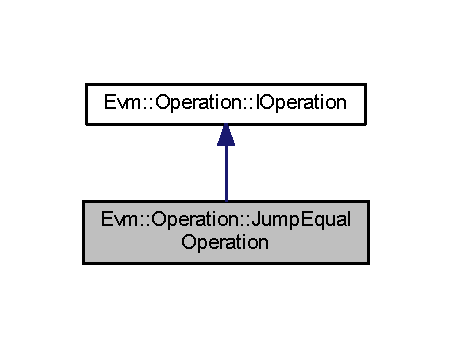
\includegraphics[width=217pt]{struct_evm_1_1_operation_1_1_jump_equal_operation__inherit__graph}
\end{center}
\end{figure}


Collaboration diagram for Evm\+:\+:Operation\+:\+:Jump\+Equal\+Operation\+:
\nopagebreak
\begin{figure}[H]
\begin{center}
\leavevmode
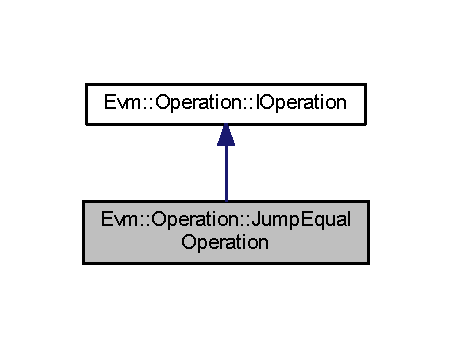
\includegraphics[width=217pt]{struct_evm_1_1_operation_1_1_jump_equal_operation__coll__graph}
\end{center}
\end{figure}
\subsection*{Public Member Functions}
\begin{DoxyCompactItemize}
\item 
virtual void \mbox{\hyperlink{struct_evm_1_1_operation_1_1_jump_equal_operation_a5edc133dd24ca78cc59203ab3ba47763}{execute}} (\mbox{\hyperlink{struct_evm_1_1_thread_context}{Thread\+Context}} \&thread) override
\begin{DoxyCompactList}\small\item\em Execution of the instruction. \end{DoxyCompactList}\item 
\mbox{\hyperlink{struct_evm_1_1_operation_1_1_jump_equal_operation_a65e98ee1b1679e12c1d1dd000ebfe937}{I\+Operation}} (string \&opcode)
\begin{DoxyCompactList}\small\item\em Constructor. \end{DoxyCompactList}\end{DoxyCompactItemize}
\subsection*{Additional Inherited Members}


\subsection{Detailed Description}
jump\+Equal operation 

jump\+Equal address, arg1, arg2; Move instruction pointer to address if arg1 == arg2. 

\subsection{Member Function Documentation}
\mbox{\Hypertarget{struct_evm_1_1_operation_1_1_jump_equal_operation_a5edc133dd24ca78cc59203ab3ba47763}\label{struct_evm_1_1_operation_1_1_jump_equal_operation_a5edc133dd24ca78cc59203ab3ba47763}} 
\index{Evm\+::\+Operation\+::\+Jump\+Equal\+Operation@{Evm\+::\+Operation\+::\+Jump\+Equal\+Operation}!execute@{execute}}
\index{execute@{execute}!Evm\+::\+Operation\+::\+Jump\+Equal\+Operation@{Evm\+::\+Operation\+::\+Jump\+Equal\+Operation}}
\subsubsection{\texorpdfstring{execute()}{execute()}}
{\footnotesize\ttfamily void Evm\+::\+Operation\+::\+Jump\+Equal\+Operation\+::execute (\begin{DoxyParamCaption}\item[{\mbox{\hyperlink{struct_evm_1_1_thread_context}{Thread\+Context}} \&}]{thread }\end{DoxyParamCaption})\hspace{0.3cm}{\ttfamily [override]}, {\ttfamily [virtual]}}



Execution of the instruction. 

May by call by an application to execute the operation. The execution requires to be awared of thread context within the operation is executed. 
\begin{DoxyParams}{Parameters}
{\em thread} & Context of \mbox{\hyperlink{namespace_evm}{Evm}} thread \\
\hline
\end{DoxyParams}


Implements \mbox{\hyperlink{struct_evm_1_1_operation_1_1_i_operation_a7285631335da103423c01471dedeb1d7}{Evm\+::\+Operation\+::\+I\+Operation}}.

\mbox{\Hypertarget{struct_evm_1_1_operation_1_1_jump_equal_operation_a65e98ee1b1679e12c1d1dd000ebfe937}\label{struct_evm_1_1_operation_1_1_jump_equal_operation_a65e98ee1b1679e12c1d1dd000ebfe937}} 
\index{Evm\+::\+Operation\+::\+Jump\+Equal\+Operation@{Evm\+::\+Operation\+::\+Jump\+Equal\+Operation}!I\+Operation@{I\+Operation}}
\index{I\+Operation@{I\+Operation}!Evm\+::\+Operation\+::\+Jump\+Equal\+Operation@{Evm\+::\+Operation\+::\+Jump\+Equal\+Operation}}
\subsubsection{\texorpdfstring{I\+Operation()}{IOperation()}}
{\footnotesize\ttfamily Evm\+::\+Operation\+::\+I\+Operation\+::\+I\+Operation\hspace{0.3cm}{\ttfamily [inline]}}



Constructor. 


\begin{DoxyParams}{Parameters}
{\em opcode} & Printable label of the instruction \\
\hline
\end{DoxyParams}


The documentation for this struct was generated from the following files\+:\begin{DoxyCompactItemize}
\item 
Evm/Operation.\+h\item 
Evm/\mbox{\hyperlink{_operation_8cpp}{Operation.\+cpp}}\end{DoxyCompactItemize}

\hypertarget{struct_evm_1_1_operation_1_1_jump_equal_operation_factory}{}\section{Evm\+:\+:Operation\+:\+:Jump\+Equal\+Operation\+Factory Struct Reference}
\label{struct_evm_1_1_operation_1_1_jump_equal_operation_factory}\index{Evm\+::\+Operation\+::\+Jump\+Equal\+Operation\+Factory@{Evm\+::\+Operation\+::\+Jump\+Equal\+Operation\+Factory}}


Inheritance diagram for Evm\+:\+:Operation\+:\+:Jump\+Equal\+Operation\+Factory\+:
\nopagebreak
\begin{figure}[H]
\begin{center}
\leavevmode
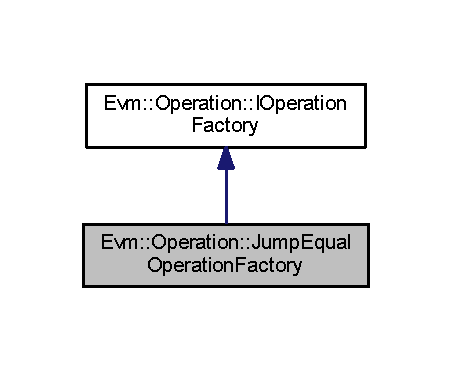
\includegraphics[width=217pt]{struct_evm_1_1_operation_1_1_jump_equal_operation_factory__inherit__graph}
\end{center}
\end{figure}


Collaboration diagram for Evm\+:\+:Operation\+:\+:Jump\+Equal\+Operation\+Factory\+:
\nopagebreak
\begin{figure}[H]
\begin{center}
\leavevmode
\includegraphics[width=228pt]{struct_evm_1_1_operation_1_1_jump_equal_operation_factory__coll__graph}
\end{center}
\end{figure}
\subsection*{Public Member Functions}
\begin{DoxyCompactItemize}
\item 
\mbox{\Hypertarget{struct_evm_1_1_operation_1_1_jump_equal_operation_factory_abac021b9a2119410e0b008d45e77bb2d}\label{struct_evm_1_1_operation_1_1_jump_equal_operation_factory_abac021b9a2119410e0b008d45e77bb2d}} 
virtual Operation\+Ptr {\bfseries build} (uint32\+\_\+t \&offset)
\item 
\mbox{\Hypertarget{struct_evm_1_1_operation_1_1_jump_equal_operation_factory_a7621b51ca2bc125b36be673486e33781}\label{struct_evm_1_1_operation_1_1_jump_equal_operation_factory_a7621b51ca2bc125b36be673486e33781}} 
{\bfseries I\+Operation\+Factory} (const string \&opcode, const \mbox{\hyperlink{struct_evm_1_1_utils_1_1_bit_buffer}{Utils\+::\+Bit\+Buffer}} \&program\+Memory)
\end{DoxyCompactItemize}
\subsection*{Additional Inherited Members}


The documentation for this struct was generated from the following files\+:\begin{DoxyCompactItemize}
\item 
Evm/Operation\+Factory.\+h\item 
Evm/Operation\+Factory.\+cpp\end{DoxyCompactItemize}

\hypertarget{struct_evm_1_1_operation_1_1_jump_operation}{}\section{Evm\+:\+:Operation\+:\+:Jump\+Operation Struct Reference}
\label{struct_evm_1_1_operation_1_1_jump_operation}\index{Evm\+::\+Operation\+::\+Jump\+Operation@{Evm\+::\+Operation\+::\+Jump\+Operation}}


jump operation  




{\ttfamily \#include $<$Operation.\+h$>$}



Inheritance diagram for Evm\+:\+:Operation\+:\+:Jump\+Operation\+:
\nopagebreak
\begin{figure}[H]
\begin{center}
\leavevmode
\includegraphics[width=235pt]{struct_evm_1_1_operation_1_1_jump_operation__inherit__graph}
\end{center}
\end{figure}


Collaboration diagram for Evm\+:\+:Operation\+:\+:Jump\+Operation\+:
\nopagebreak
\begin{figure}[H]
\begin{center}
\leavevmode
\includegraphics[width=235pt]{struct_evm_1_1_operation_1_1_jump_operation__coll__graph}
\end{center}
\end{figure}
\subsection*{Public Member Functions}
\begin{DoxyCompactItemize}
\item 
virtual void \mbox{\hyperlink{struct_evm_1_1_operation_1_1_jump_operation_a830ab356fc212ff9ace8b63b0d24dcb1}{execute}} (\mbox{\hyperlink{struct_evm_1_1_thread_context}{Thread\+Context}} \&thread) override
\begin{DoxyCompactList}\small\item\em Execution of the instruction. \end{DoxyCompactList}\item 
\mbox{\hyperlink{struct_evm_1_1_operation_1_1_jump_operation_a65e98ee1b1679e12c1d1dd000ebfe937}{I\+Operation}} (string \&opcode)
\begin{DoxyCompactList}\small\item\em Constructor. \end{DoxyCompactList}\end{DoxyCompactItemize}
\subsection*{Additional Inherited Members}


\subsection{Detailed Description}
jump operation 

jump address; Move instruction pointer to address 

\subsection{Member Function Documentation}
\mbox{\Hypertarget{struct_evm_1_1_operation_1_1_jump_operation_a830ab356fc212ff9ace8b63b0d24dcb1}\label{struct_evm_1_1_operation_1_1_jump_operation_a830ab356fc212ff9ace8b63b0d24dcb1}} 
\index{Evm\+::\+Operation\+::\+Jump\+Operation@{Evm\+::\+Operation\+::\+Jump\+Operation}!execute@{execute}}
\index{execute@{execute}!Evm\+::\+Operation\+::\+Jump\+Operation@{Evm\+::\+Operation\+::\+Jump\+Operation}}
\subsubsection{\texorpdfstring{execute()}{execute()}}
{\footnotesize\ttfamily void Evm\+::\+Operation\+::\+Jump\+Operation\+::execute (\begin{DoxyParamCaption}\item[{\mbox{\hyperlink{struct_evm_1_1_thread_context}{Thread\+Context}} \&}]{thread }\end{DoxyParamCaption})\hspace{0.3cm}{\ttfamily [override]}, {\ttfamily [virtual]}}



Execution of the instruction. 

May by call by an application to execute the operation. The execution requires to be awared of thread context within the operation is executed. 
\begin{DoxyParams}{Parameters}
{\em thread} & Context of \mbox{\hyperlink{namespace_evm}{Evm}} thread \\
\hline
\end{DoxyParams}


Implements \mbox{\hyperlink{struct_evm_1_1_operation_1_1_i_operation_a7285631335da103423c01471dedeb1d7}{Evm\+::\+Operation\+::\+I\+Operation}}.

\mbox{\Hypertarget{struct_evm_1_1_operation_1_1_jump_operation_a65e98ee1b1679e12c1d1dd000ebfe937}\label{struct_evm_1_1_operation_1_1_jump_operation_a65e98ee1b1679e12c1d1dd000ebfe937}} 
\index{Evm\+::\+Operation\+::\+Jump\+Operation@{Evm\+::\+Operation\+::\+Jump\+Operation}!I\+Operation@{I\+Operation}}
\index{I\+Operation@{I\+Operation}!Evm\+::\+Operation\+::\+Jump\+Operation@{Evm\+::\+Operation\+::\+Jump\+Operation}}
\subsubsection{\texorpdfstring{I\+Operation()}{IOperation()}}
{\footnotesize\ttfamily Evm\+::\+Operation\+::\+I\+Operation\+::\+I\+Operation\hspace{0.3cm}{\ttfamily [inline]}}



Constructor. 


\begin{DoxyParams}{Parameters}
{\em opcode} & Printable label of the instruction \\
\hline
\end{DoxyParams}


The documentation for this struct was generated from the following files\+:\begin{DoxyCompactItemize}
\item 
Evm/Operation.\+h\item 
Evm/\mbox{\hyperlink{_operation_8cpp}{Operation.\+cpp}}\end{DoxyCompactItemize}

\hypertarget{struct_evm_1_1_operation_1_1_load_const_operation}{}\section{Evm\+:\+:Operation\+:\+:Load\+Const\+Operation Struct Reference}
\label{struct_evm_1_1_operation_1_1_load_const_operation}\index{Evm\+::\+Operation\+::\+Load\+Const\+Operation@{Evm\+::\+Operation\+::\+Load\+Const\+Operation}}


load\+Const operation  




{\ttfamily \#include $<$Operation.\+h$>$}



Inheritance diagram for Evm\+:\+:Operation\+:\+:Load\+Const\+Operation\+:
\nopagebreak
\begin{figure}[H]
\begin{center}
\leavevmode
\includegraphics[width=216pt]{struct_evm_1_1_operation_1_1_load_const_operation__inherit__graph}
\end{center}
\end{figure}


Collaboration diagram for Evm\+:\+:Operation\+:\+:Load\+Const\+Operation\+:
\nopagebreak
\begin{figure}[H]
\begin{center}
\leavevmode
\includegraphics[width=216pt]{struct_evm_1_1_operation_1_1_load_const_operation__coll__graph}
\end{center}
\end{figure}
\subsection*{Public Member Functions}
\begin{DoxyCompactItemize}
\item 
virtual void \mbox{\hyperlink{struct_evm_1_1_operation_1_1_load_const_operation_a434d2748c59ccf0e3d1977e87c110e15}{execute}} (\mbox{\hyperlink{struct_evm_1_1_thread_context}{Thread\+Context}} \&thread) override
\begin{DoxyCompactList}\small\item\em Execution of the instruction. \end{DoxyCompactList}\item 
\mbox{\hyperlink{struct_evm_1_1_operation_1_1_load_const_operation_a65e98ee1b1679e12c1d1dd000ebfe937}{I\+Operation}} (string \&opcode)
\begin{DoxyCompactList}\small\item\em Constructor. \end{DoxyCompactList}\end{DoxyCompactItemize}
\subsection*{Additional Inherited Members}


\subsection{Detailed Description}
load\+Const operation 

load\+Const constant, arg1; arg1 $<$-\/constant 

\subsection{Member Function Documentation}
\mbox{\Hypertarget{struct_evm_1_1_operation_1_1_load_const_operation_a434d2748c59ccf0e3d1977e87c110e15}\label{struct_evm_1_1_operation_1_1_load_const_operation_a434d2748c59ccf0e3d1977e87c110e15}} 
\index{Evm\+::\+Operation\+::\+Load\+Const\+Operation@{Evm\+::\+Operation\+::\+Load\+Const\+Operation}!execute@{execute}}
\index{execute@{execute}!Evm\+::\+Operation\+::\+Load\+Const\+Operation@{Evm\+::\+Operation\+::\+Load\+Const\+Operation}}
\subsubsection{\texorpdfstring{execute()}{execute()}}
{\footnotesize\ttfamily void Evm\+::\+Operation\+::\+Load\+Const\+Operation\+::execute (\begin{DoxyParamCaption}\item[{\mbox{\hyperlink{struct_evm_1_1_thread_context}{Thread\+Context}} \&}]{thread }\end{DoxyParamCaption})\hspace{0.3cm}{\ttfamily [override]}, {\ttfamily [virtual]}}



Execution of the instruction. 

May by call by an application to execute the operation. The execution requires to be awared of thread context within the operation is executed. 
\begin{DoxyParams}{Parameters}
{\em thread} & Context of \mbox{\hyperlink{namespace_evm}{Evm}} thread \\
\hline
\end{DoxyParams}


Implements \mbox{\hyperlink{struct_evm_1_1_operation_1_1_i_operation_a7285631335da103423c01471dedeb1d7}{Evm\+::\+Operation\+::\+I\+Operation}}.

\mbox{\Hypertarget{struct_evm_1_1_operation_1_1_load_const_operation_a65e98ee1b1679e12c1d1dd000ebfe937}\label{struct_evm_1_1_operation_1_1_load_const_operation_a65e98ee1b1679e12c1d1dd000ebfe937}} 
\index{Evm\+::\+Operation\+::\+Load\+Const\+Operation@{Evm\+::\+Operation\+::\+Load\+Const\+Operation}!I\+Operation@{I\+Operation}}
\index{I\+Operation@{I\+Operation}!Evm\+::\+Operation\+::\+Load\+Const\+Operation@{Evm\+::\+Operation\+::\+Load\+Const\+Operation}}
\subsubsection{\texorpdfstring{I\+Operation()}{IOperation()}}
{\footnotesize\ttfamily Evm\+::\+Operation\+::\+I\+Operation\+::\+I\+Operation\hspace{0.3cm}{\ttfamily [inline]}}



Constructor. 


\begin{DoxyParams}{Parameters}
{\em opcode} & Printable label of the instruction \\
\hline
\end{DoxyParams}


The documentation for this struct was generated from the following files\+:\begin{DoxyCompactItemize}
\item 
Evm/Operation.\+h\item 
Evm/\mbox{\hyperlink{_operation_8cpp}{Operation.\+cpp}}\end{DoxyCompactItemize}

\hypertarget{struct_evm_1_1_operation_1_1_load_const_operation_factory}{}\section{Evm\+:\+:Operation\+:\+:Load\+Const\+Operation\+Factory Struct Reference}
\label{struct_evm_1_1_operation_1_1_load_const_operation_factory}\index{Evm\+::\+Operation\+::\+Load\+Const\+Operation\+Factory@{Evm\+::\+Operation\+::\+Load\+Const\+Operation\+Factory}}


Inheritance diagram for Evm\+:\+:Operation\+:\+:Load\+Const\+Operation\+Factory\+:
\nopagebreak
\begin{figure}[H]
\begin{center}
\leavevmode
\includegraphics[width=216pt]{struct_evm_1_1_operation_1_1_load_const_operation_factory__inherit__graph}
\end{center}
\end{figure}


Collaboration diagram for Evm\+:\+:Operation\+:\+:Load\+Const\+Operation\+Factory\+:
\nopagebreak
\begin{figure}[H]
\begin{center}
\leavevmode
\includegraphics[width=227pt]{struct_evm_1_1_operation_1_1_load_const_operation_factory__coll__graph}
\end{center}
\end{figure}
\subsection*{Public Member Functions}
\begin{DoxyCompactItemize}
\item 
\mbox{\Hypertarget{struct_evm_1_1_operation_1_1_load_const_operation_factory_a9183214276b6e4fc6b74523fb7775df0}\label{struct_evm_1_1_operation_1_1_load_const_operation_factory_a9183214276b6e4fc6b74523fb7775df0}} 
virtual Operation\+Ptr {\bfseries build} (uint32\+\_\+t \&offset)
\item 
\mbox{\Hypertarget{struct_evm_1_1_operation_1_1_load_const_operation_factory_a7621b51ca2bc125b36be673486e33781}\label{struct_evm_1_1_operation_1_1_load_const_operation_factory_a7621b51ca2bc125b36be673486e33781}} 
{\bfseries I\+Operation\+Factory} (const string \&opcode, const \mbox{\hyperlink{struct_evm_1_1_utils_1_1_bit_buffer}{Utils\+::\+Bit\+Buffer}} \&program\+Memory)
\end{DoxyCompactItemize}
\subsection*{Additional Inherited Members}


The documentation for this struct was generated from the following files\+:\begin{DoxyCompactItemize}
\item 
Evm/Operation\+Factory.\+h\item 
Evm/Operation\+Factory.\+cpp\end{DoxyCompactItemize}

\hypertarget{struct_evm_1_1_operation_1_1_lock_operation}{}\section{Evm\+:\+:Operation\+:\+:Lock\+Operation Struct Reference}
\label{struct_evm_1_1_operation_1_1_lock_operation}\index{Evm\+::\+Operation\+::\+Lock\+Operation@{Evm\+::\+Operation\+::\+Lock\+Operation}}


lock operation  




{\ttfamily \#include $<$Operation.\+h$>$}



Inheritance diagram for Evm\+:\+:Operation\+:\+:Lock\+Operation\+:
\nopagebreak
\begin{figure}[H]
\begin{center}
\leavevmode
\includegraphics[width=232pt]{struct_evm_1_1_operation_1_1_lock_operation__inherit__graph}
\end{center}
\end{figure}


Collaboration diagram for Evm\+:\+:Operation\+:\+:Lock\+Operation\+:
\nopagebreak
\begin{figure}[H]
\begin{center}
\leavevmode
\includegraphics[width=232pt]{struct_evm_1_1_operation_1_1_lock_operation__coll__graph}
\end{center}
\end{figure}
\subsection*{Public Member Functions}
\begin{DoxyCompactItemize}
\item 
virtual void \mbox{\hyperlink{struct_evm_1_1_operation_1_1_lock_operation_a2ecf10dec9abb8203f56a8f119a97a7f}{execute}} (\mbox{\hyperlink{struct_evm_1_1_thread_context}{Thread\+Context}} \&thread) override
\begin{DoxyCompactList}\small\item\em Execution of the instruction. \end{DoxyCompactList}\item 
\mbox{\hyperlink{struct_evm_1_1_operation_1_1_lock_operation_a65e98ee1b1679e12c1d1dd000ebfe937}{I\+Operation}} (string \&opcode)
\begin{DoxyCompactList}\small\item\em Constructor. \end{DoxyCompactList}\end{DoxyCompactItemize}
\subsection*{Additional Inherited Members}


\subsection{Detailed Description}
lock operation 

lock arg1; Lock synchronization object identified by arg1 

\subsection{Member Function Documentation}
\mbox{\Hypertarget{struct_evm_1_1_operation_1_1_lock_operation_a2ecf10dec9abb8203f56a8f119a97a7f}\label{struct_evm_1_1_operation_1_1_lock_operation_a2ecf10dec9abb8203f56a8f119a97a7f}} 
\index{Evm\+::\+Operation\+::\+Lock\+Operation@{Evm\+::\+Operation\+::\+Lock\+Operation}!execute@{execute}}
\index{execute@{execute}!Evm\+::\+Operation\+::\+Lock\+Operation@{Evm\+::\+Operation\+::\+Lock\+Operation}}
\subsubsection{\texorpdfstring{execute()}{execute()}}
{\footnotesize\ttfamily void Evm\+::\+Operation\+::\+Lock\+Operation\+::execute (\begin{DoxyParamCaption}\item[{\mbox{\hyperlink{struct_evm_1_1_thread_context}{Thread\+Context}} \&}]{thread }\end{DoxyParamCaption})\hspace{0.3cm}{\ttfamily [override]}, {\ttfamily [virtual]}}



Execution of the instruction. 

May by call by an application to execute the operation. The execution requires to be awared of thread context within the operation is executed. 
\begin{DoxyParams}{Parameters}
{\em thread} & Context of \mbox{\hyperlink{namespace_evm}{Evm}} thread \\
\hline
\end{DoxyParams}


Implements \mbox{\hyperlink{struct_evm_1_1_operation_1_1_i_operation_a7285631335da103423c01471dedeb1d7}{Evm\+::\+Operation\+::\+I\+Operation}}.

\mbox{\Hypertarget{struct_evm_1_1_operation_1_1_lock_operation_a65e98ee1b1679e12c1d1dd000ebfe937}\label{struct_evm_1_1_operation_1_1_lock_operation_a65e98ee1b1679e12c1d1dd000ebfe937}} 
\index{Evm\+::\+Operation\+::\+Lock\+Operation@{Evm\+::\+Operation\+::\+Lock\+Operation}!I\+Operation@{I\+Operation}}
\index{I\+Operation@{I\+Operation}!Evm\+::\+Operation\+::\+Lock\+Operation@{Evm\+::\+Operation\+::\+Lock\+Operation}}
\subsubsection{\texorpdfstring{I\+Operation()}{IOperation()}}
{\footnotesize\ttfamily Evm\+::\+Operation\+::\+I\+Operation\+::\+I\+Operation\hspace{0.3cm}{\ttfamily [inline]}}



Constructor. 


\begin{DoxyParams}{Parameters}
{\em opcode} & Printable label of the instruction \\
\hline
\end{DoxyParams}


The documentation for this struct was generated from the following files\+:\begin{DoxyCompactItemize}
\item 
Evm/Operation.\+h\item 
Evm/\mbox{\hyperlink{_operation_8cpp}{Operation.\+cpp}}\end{DoxyCompactItemize}

\hypertarget{struct_evm_1_1_operation_1_1_math_operation}{}\section{Evm\+:\+:Operation\+:\+:Math\+Operation Struct Reference}
\label{struct_evm_1_1_operation_1_1_math_operation}\index{Evm\+::\+Operation\+::\+Math\+Operation@{Evm\+::\+Operation\+::\+Math\+Operation}}


\mbox{\hyperlink{struct_evm_1_1_operation_1_1_math_operation}{Math\+Operation}} Interface.  




{\ttfamily \#include $<$Operation.\+h$>$}



Inheritance diagram for Evm\+:\+:Operation\+:\+:Math\+Operation\+:
\nopagebreak
\begin{figure}[H]
\begin{center}
\leavevmode
\includegraphics[width=233pt]{struct_evm_1_1_operation_1_1_math_operation__inherit__graph}
\end{center}
\end{figure}


Collaboration diagram for Evm\+:\+:Operation\+:\+:Math\+Operation\+:
\nopagebreak
\begin{figure}[H]
\begin{center}
\leavevmode
\includegraphics[width=233pt]{struct_evm_1_1_operation_1_1_math_operation__coll__graph}
\end{center}
\end{figure}
\subsection*{Public Member Functions}
\begin{DoxyCompactItemize}
\item 
\mbox{\hyperlink{struct_evm_1_1_operation_1_1_math_operation_a039f3663ce4a0b579c19e1d236d81cd5}{Math\+Operation}} (string \&opcode, function$<$ int64\+\_\+t(int64\+\_\+t, int64\+\_\+t)$>$ math\+Operation)
\begin{DoxyCompactList}\small\item\em Constructor. \end{DoxyCompactList}\item 
virtual void \mbox{\hyperlink{struct_evm_1_1_operation_1_1_math_operation_a5ffc66e4ff4e6f59b1cd2512aad54380}{execute}} (\mbox{\hyperlink{struct_evm_1_1_thread_context}{Thread\+Context}} \&thread) override
\begin{DoxyCompactList}\small\item\em Execution of the instruction. \end{DoxyCompactList}\end{DoxyCompactItemize}
\subsection*{Additional Inherited Members}


\subsection{Detailed Description}
\mbox{\hyperlink{struct_evm_1_1_operation_1_1_math_operation}{Math\+Operation}} Interface. 

Math operation if a subinterface of \mbox{\hyperlink{struct_evm_1_1_operation_1_1_i_operation}{I\+Operation}} that can execute mathematic instructions. It is good for three-\/argument operations like follows\+: arg3 $<$-\/ arg1 \# arg2 where \# is function given by an user. The interface takes lambda as an argument. At the moment the following instructions are implemented with this interface\+: add, sub, mul, dev, compare 

\subsection{Constructor \& Destructor Documentation}
\mbox{\Hypertarget{struct_evm_1_1_operation_1_1_math_operation_a039f3663ce4a0b579c19e1d236d81cd5}\label{struct_evm_1_1_operation_1_1_math_operation_a039f3663ce4a0b579c19e1d236d81cd5}} 
\index{Evm\+::\+Operation\+::\+Math\+Operation@{Evm\+::\+Operation\+::\+Math\+Operation}!Math\+Operation@{Math\+Operation}}
\index{Math\+Operation@{Math\+Operation}!Evm\+::\+Operation\+::\+Math\+Operation@{Evm\+::\+Operation\+::\+Math\+Operation}}
\subsubsection{\texorpdfstring{Math\+Operation()}{MathOperation()}}
{\footnotesize\ttfamily Evm\+::\+Operation\+::\+Math\+Operation\+::\+Math\+Operation (\begin{DoxyParamCaption}\item[{string \&}]{opcode,  }\item[{function$<$ int64\+\_\+t(int64\+\_\+t, int64\+\_\+t)$>$}]{math\+Operation }\end{DoxyParamCaption})\hspace{0.3cm}{\ttfamily [inline]}}



Constructor. 


\begin{DoxyParams}{Parameters}
{\em opcode} & Printable label of the instruction \\
\hline
{\em function} & Lambde with the essental operation \\
\hline
\end{DoxyParams}


\subsection{Member Function Documentation}
\mbox{\Hypertarget{struct_evm_1_1_operation_1_1_math_operation_a5ffc66e4ff4e6f59b1cd2512aad54380}\label{struct_evm_1_1_operation_1_1_math_operation_a5ffc66e4ff4e6f59b1cd2512aad54380}} 
\index{Evm\+::\+Operation\+::\+Math\+Operation@{Evm\+::\+Operation\+::\+Math\+Operation}!execute@{execute}}
\index{execute@{execute}!Evm\+::\+Operation\+::\+Math\+Operation@{Evm\+::\+Operation\+::\+Math\+Operation}}
\subsubsection{\texorpdfstring{execute()}{execute()}}
{\footnotesize\ttfamily void Evm\+::\+Operation\+::\+Math\+Operation\+::execute (\begin{DoxyParamCaption}\item[{\mbox{\hyperlink{struct_evm_1_1_thread_context}{Thread\+Context}} \&}]{thread }\end{DoxyParamCaption})\hspace{0.3cm}{\ttfamily [override]}, {\ttfamily [virtual]}}



Execution of the instruction. 

May by call by an application to execute the operation. The execution requires to be awared of thread context within the operation is executed. 
\begin{DoxyParams}{Parameters}
{\em thread} & Context of \mbox{\hyperlink{namespace_evm}{Evm}} thread \\
\hline
\end{DoxyParams}


Implements \mbox{\hyperlink{struct_evm_1_1_operation_1_1_i_operation_a7285631335da103423c01471dedeb1d7}{Evm\+::\+Operation\+::\+I\+Operation}}.



The documentation for this struct was generated from the following files\+:\begin{DoxyCompactItemize}
\item 
Evm/Operation.\+h\item 
Evm/\mbox{\hyperlink{_operation_8cpp}{Operation.\+cpp}}\end{DoxyCompactItemize}

\hypertarget{struct_evm_1_1_operation_1_1_math_operation_factory}{}\section{Evm\+:\+:Operation\+:\+:Math\+Operation\+Factory Struct Reference}
\label{struct_evm_1_1_operation_1_1_math_operation_factory}\index{Evm\+::\+Operation\+::\+Math\+Operation\+Factory@{Evm\+::\+Operation\+::\+Math\+Operation\+Factory}}


Inheritance diagram for Evm\+:\+:Operation\+:\+:Math\+Operation\+Factory\+:
\nopagebreak
\begin{figure}[H]
\begin{center}
\leavevmode
\includegraphics[width=233pt]{struct_evm_1_1_operation_1_1_math_operation_factory__inherit__graph}
\end{center}
\end{figure}


Collaboration diagram for Evm\+:\+:Operation\+:\+:Math\+Operation\+Factory\+:
\nopagebreak
\begin{figure}[H]
\begin{center}
\leavevmode
\includegraphics[width=236pt]{struct_evm_1_1_operation_1_1_math_operation_factory__coll__graph}
\end{center}
\end{figure}
\subsection*{Public Member Functions}
\begin{DoxyCompactItemize}
\item 
\mbox{\Hypertarget{struct_evm_1_1_operation_1_1_math_operation_factory_a34cc15fc9a323bb761c71301db56c28b}\label{struct_evm_1_1_operation_1_1_math_operation_factory_a34cc15fc9a323bb761c71301db56c28b}} 
{\bfseries Math\+Operation\+Factory} (const string \&opcode, const \mbox{\hyperlink{struct_evm_1_1_utils_1_1_bit_buffer}{Utils\+::\+Bit\+Buffer}} \&bb, function$<$ int64\+\_\+t(int64\+\_\+t, int64\+\_\+t)$>$ function)
\item 
\mbox{\Hypertarget{struct_evm_1_1_operation_1_1_math_operation_factory_ae4858379ee6817de0b2ac94a6d539e6e}\label{struct_evm_1_1_operation_1_1_math_operation_factory_ae4858379ee6817de0b2ac94a6d539e6e}} 
Operation\+Ptr {\bfseries build} (uint32\+\_\+t \&offset)
\end{DoxyCompactItemize}
\subsection*{Additional Inherited Members}


The documentation for this struct was generated from the following files\+:\begin{DoxyCompactItemize}
\item 
Evm/Operation\+Factory.\+h\item 
Evm/Operation\+Factory.\+cpp\end{DoxyCompactItemize}

\hypertarget{struct_evm_1_1_utils_1_1_memory}{}\section{Evm\+:\+:Utils\+:\+:Memory Struct Reference}
\label{struct_evm_1_1_utils_1_1_memory}\index{Evm\+::\+Utils\+::\+Memory@{Evm\+::\+Utils\+::\+Memory}}
\subsection*{Public Member Functions}
\begin{DoxyCompactItemize}
\item 
\mbox{\Hypertarget{struct_evm_1_1_utils_1_1_memory_ab8d1267eafa00ba1401104a42cbb66bd}\label{struct_evm_1_1_utils_1_1_memory_ab8d1267eafa00ba1401104a42cbb66bd}} 
{\bfseries Memory} (uint64\+\_\+t size)
\item 
\mbox{\Hypertarget{struct_evm_1_1_utils_1_1_memory_abf86e5fe3a3bedf2ead48a8d432b5789}\label{struct_evm_1_1_utils_1_1_memory_abf86e5fe3a3bedf2ead48a8d432b5789}} 
void {\bfseries write} (uint64\+\_\+t address, const Bytes \&data)
\item 
\mbox{\Hypertarget{struct_evm_1_1_utils_1_1_memory_a2a259165924fd686ffa44224568cf245}\label{struct_evm_1_1_utils_1_1_memory_a2a259165924fd686ffa44224568cf245}} 
void {\bfseries write} (uint64\+\_\+t address, Bytes\+::const\+\_\+iterator beg, Bytes\+::const\+\_\+iterator end)
\item 
\mbox{\Hypertarget{struct_evm_1_1_utils_1_1_memory_a8d00216c4981ac8c5e86726614ce44cb}\label{struct_evm_1_1_utils_1_1_memory_a8d00216c4981ac8c5e86726614ce44cb}} 
Bytes {\bfseries read} (uint64\+\_\+t address, uint64\+\_\+t size) const
\end{DoxyCompactItemize}


The documentation for this struct was generated from the following files\+:\begin{DoxyCompactItemize}
\item 
Evm/Memory.\+h\item 
Evm/Memory.\+cpp\end{DoxyCompactItemize}

\hypertarget{struct_evm_1_1_argument_1_1_memory_b_y_t_e_argument}{}\section{Evm\+:\+:Argument\+:\+:Memory\+B\+Y\+T\+E\+Argument Struct Reference}
\label{struct_evm_1_1_argument_1_1_memory_b_y_t_e_argument}\index{Evm\+::\+Argument\+::\+Memory\+B\+Y\+T\+E\+Argument@{Evm\+::\+Argument\+::\+Memory\+B\+Y\+T\+E\+Argument}}


Inheritance diagram for Evm\+:\+:Argument\+:\+:Memory\+B\+Y\+T\+E\+Argument\+:
\nopagebreak
\begin{figure}[H]
\begin{center}
\leavevmode
\includegraphics[width=272pt]{struct_evm_1_1_argument_1_1_memory_b_y_t_e_argument__inherit__graph}
\end{center}
\end{figure}


Collaboration diagram for Evm\+:\+:Argument\+:\+:Memory\+B\+Y\+T\+E\+Argument\+:
\nopagebreak
\begin{figure}[H]
\begin{center}
\leavevmode
\includegraphics[width=272pt]{struct_evm_1_1_argument_1_1_memory_b_y_t_e_argument__coll__graph}
\end{center}
\end{figure}
\subsection*{Public Member Functions}
\begin{DoxyCompactItemize}
\item 
virtual uint64\+\_\+t \mbox{\hyperlink{struct_evm_1_1_argument_1_1_memory_b_y_t_e_argument_af038f3d7e425ef70f5688bda45eb8d31}{get\+Value}} (\mbox{\hyperlink{struct_evm_1_1_thread_context}{Thread\+Context}} \&thread) const override
\begin{DoxyCompactList}\small\item\em Get value. \end{DoxyCompactList}\item 
virtual void \mbox{\hyperlink{struct_evm_1_1_argument_1_1_memory_b_y_t_e_argument_a6da25d3c59f1676c39ac8f0f0f211863}{set\+Value}} (\mbox{\hyperlink{struct_evm_1_1_thread_context}{Thread\+Context}} \&thread, uint64\+\_\+t value) override
\begin{DoxyCompactList}\small\item\em Set value. \end{DoxyCompactList}\item 
virtual string \mbox{\hyperlink{struct_evm_1_1_argument_1_1_memory_b_y_t_e_argument_afbe889873f7f6c825d9554e2029294b3}{label}} () const override
\begin{DoxyCompactList}\small\item\em Get printable representation of the argument. \end{DoxyCompactList}\item 
virtual string \mbox{\hyperlink{struct_evm_1_1_argument_1_1_memory_b_y_t_e_argument_a7fbed3cafe6784094617c522a2c91412}{print\+Value}} (\mbox{\hyperlink{struct_evm_1_1_thread_context}{Thread\+Context}} \&thread) const override
\begin{DoxyCompactList}\small\item\em Get printable value of the parameter. \end{DoxyCompactList}\item 
\mbox{\Hypertarget{struct_evm_1_1_argument_1_1_memory_b_y_t_e_argument_aa3dfe476b956a51bb26409c1d8763e21}\label{struct_evm_1_1_argument_1_1_memory_b_y_t_e_argument_aa3dfe476b956a51bb26409c1d8763e21}} 
{\bfseries I\+Register\+Base\+Argument} (uint8\+\_\+t register\+Index)
\end{DoxyCompactItemize}
\subsection*{Additional Inherited Members}


\subsection{Member Function Documentation}
\mbox{\Hypertarget{struct_evm_1_1_argument_1_1_memory_b_y_t_e_argument_af038f3d7e425ef70f5688bda45eb8d31}\label{struct_evm_1_1_argument_1_1_memory_b_y_t_e_argument_af038f3d7e425ef70f5688bda45eb8d31}} 
\index{Evm\+::\+Argument\+::\+Memory\+B\+Y\+T\+E\+Argument@{Evm\+::\+Argument\+::\+Memory\+B\+Y\+T\+E\+Argument}!get\+Value@{get\+Value}}
\index{get\+Value@{get\+Value}!Evm\+::\+Argument\+::\+Memory\+B\+Y\+T\+E\+Argument@{Evm\+::\+Argument\+::\+Memory\+B\+Y\+T\+E\+Argument}}
\subsubsection{\texorpdfstring{get\+Value()}{getValue()}}
{\footnotesize\ttfamily uint64\+\_\+t Evm\+::\+Argument\+::\+Memory\+B\+Y\+T\+E\+Argument\+::get\+Value (\begin{DoxyParamCaption}\item[{\mbox{\hyperlink{struct_evm_1_1_thread_context}{Thread\+Context}} \&}]{thread }\end{DoxyParamCaption}) const\hspace{0.3cm}{\ttfamily [override]}, {\ttfamily [virtual]}}



Get value. 

Return value of the argument 
\begin{DoxyParams}{Parameters}
{\em thread} & Thread context within this argument is used \\
\hline
\end{DoxyParams}
\begin{DoxyReturn}{Returns}
Value of the parameter 
\end{DoxyReturn}


Implements \mbox{\hyperlink{struct_evm_1_1_argument_1_1_i_argument_af01db10f34498344831877847c2fc038}{Evm\+::\+Argument\+::\+I\+Argument}}.

\mbox{\Hypertarget{struct_evm_1_1_argument_1_1_memory_b_y_t_e_argument_afbe889873f7f6c825d9554e2029294b3}\label{struct_evm_1_1_argument_1_1_memory_b_y_t_e_argument_afbe889873f7f6c825d9554e2029294b3}} 
\index{Evm\+::\+Argument\+::\+Memory\+B\+Y\+T\+E\+Argument@{Evm\+::\+Argument\+::\+Memory\+B\+Y\+T\+E\+Argument}!label@{label}}
\index{label@{label}!Evm\+::\+Argument\+::\+Memory\+B\+Y\+T\+E\+Argument@{Evm\+::\+Argument\+::\+Memory\+B\+Y\+T\+E\+Argument}}
\subsubsection{\texorpdfstring{label()}{label()}}
{\footnotesize\ttfamily string Evm\+::\+Argument\+::\+Memory\+B\+Y\+T\+E\+Argument\+::label (\begin{DoxyParamCaption}{ }\end{DoxyParamCaption}) const\hspace{0.3cm}{\ttfamily [override]}, {\ttfamily [virtual]}}



Get printable representation of the argument. 

\begin{DoxyReturn}{Returns}
string with argument label 
\end{DoxyReturn}


Implements \mbox{\hyperlink{struct_evm_1_1_argument_1_1_i_argument_a35bdae816e89f6f9fc393b6e03c5e521}{Evm\+::\+Argument\+::\+I\+Argument}}.

\mbox{\Hypertarget{struct_evm_1_1_argument_1_1_memory_b_y_t_e_argument_a7fbed3cafe6784094617c522a2c91412}\label{struct_evm_1_1_argument_1_1_memory_b_y_t_e_argument_a7fbed3cafe6784094617c522a2c91412}} 
\index{Evm\+::\+Argument\+::\+Memory\+B\+Y\+T\+E\+Argument@{Evm\+::\+Argument\+::\+Memory\+B\+Y\+T\+E\+Argument}!print\+Value@{print\+Value}}
\index{print\+Value@{print\+Value}!Evm\+::\+Argument\+::\+Memory\+B\+Y\+T\+E\+Argument@{Evm\+::\+Argument\+::\+Memory\+B\+Y\+T\+E\+Argument}}
\subsubsection{\texorpdfstring{print\+Value()}{printValue()}}
{\footnotesize\ttfamily string Evm\+::\+Argument\+::\+Memory\+B\+Y\+T\+E\+Argument\+::print\+Value (\begin{DoxyParamCaption}\item[{\mbox{\hyperlink{struct_evm_1_1_thread_context}{Thread\+Context}} \&}]{thread }\end{DoxyParamCaption}) const\hspace{0.3cm}{\ttfamily [override]}, {\ttfamily [virtual]}}



Get printable value of the parameter. 


\begin{DoxyParams}{Parameters}
{\em thread} & Thread context within this argument is used \\
\hline
\end{DoxyParams}
\begin{DoxyReturn}{Returns}
string with argument value 
\end{DoxyReturn}


Implements \mbox{\hyperlink{struct_evm_1_1_argument_1_1_i_argument_afcab2d2a1515518a111881a635c83da3}{Evm\+::\+Argument\+::\+I\+Argument}}.

\mbox{\Hypertarget{struct_evm_1_1_argument_1_1_memory_b_y_t_e_argument_a6da25d3c59f1676c39ac8f0f0f211863}\label{struct_evm_1_1_argument_1_1_memory_b_y_t_e_argument_a6da25d3c59f1676c39ac8f0f0f211863}} 
\index{Evm\+::\+Argument\+::\+Memory\+B\+Y\+T\+E\+Argument@{Evm\+::\+Argument\+::\+Memory\+B\+Y\+T\+E\+Argument}!set\+Value@{set\+Value}}
\index{set\+Value@{set\+Value}!Evm\+::\+Argument\+::\+Memory\+B\+Y\+T\+E\+Argument@{Evm\+::\+Argument\+::\+Memory\+B\+Y\+T\+E\+Argument}}
\subsubsection{\texorpdfstring{set\+Value()}{setValue()}}
{\footnotesize\ttfamily void Evm\+::\+Argument\+::\+Memory\+B\+Y\+T\+E\+Argument\+::set\+Value (\begin{DoxyParamCaption}\item[{\mbox{\hyperlink{struct_evm_1_1_thread_context}{Thread\+Context}} \&}]{thread,  }\item[{uint64\+\_\+t}]{value }\end{DoxyParamCaption})\hspace{0.3cm}{\ttfamily [override]}, {\ttfamily [virtual]}}



Set value. 

Set value of the argument. \begin{DoxyWarning}{Warning}
For read-\/only arguments this throws an exception 
\end{DoxyWarning}

\begin{DoxyParams}{Parameters}
{\em thread} & Thread context within this argument is used \\
\hline
{\em value} & New value of the parameter \\
\hline
\end{DoxyParams}


Implements \mbox{\hyperlink{struct_evm_1_1_argument_1_1_i_argument_a24e4c76f2750e664e3895d2ff4b9146d}{Evm\+::\+Argument\+::\+I\+Argument}}.



The documentation for this struct was generated from the following files\+:\begin{DoxyCompactItemize}
\item 
Evm/\mbox{\hyperlink{_argument_8h}{Argument.\+h}}\item 
Evm/Argument.\+cpp\end{DoxyCompactItemize}

\hypertarget{struct_evm_1_1_argument_1_1_memory_d_w_o_r_d_argument}{}\section{Evm\+:\+:Argument\+:\+:Memory\+D\+W\+O\+R\+D\+Argument Struct Reference}
\label{struct_evm_1_1_argument_1_1_memory_d_w_o_r_d_argument}\index{Evm\+::\+Argument\+::\+Memory\+D\+W\+O\+R\+D\+Argument@{Evm\+::\+Argument\+::\+Memory\+D\+W\+O\+R\+D\+Argument}}


Inheritance diagram for Evm\+:\+:Argument\+:\+:Memory\+D\+W\+O\+R\+D\+Argument\+:
\nopagebreak
\begin{figure}[H]
\begin{center}
\leavevmode
\includegraphics[width=284pt]{struct_evm_1_1_argument_1_1_memory_d_w_o_r_d_argument__inherit__graph}
\end{center}
\end{figure}


Collaboration diagram for Evm\+:\+:Argument\+:\+:Memory\+D\+W\+O\+R\+D\+Argument\+:
\nopagebreak
\begin{figure}[H]
\begin{center}
\leavevmode
\includegraphics[width=284pt]{struct_evm_1_1_argument_1_1_memory_d_w_o_r_d_argument__coll__graph}
\end{center}
\end{figure}
\subsection*{Public Member Functions}
\begin{DoxyCompactItemize}
\item 
virtual uint64\+\_\+t \mbox{\hyperlink{struct_evm_1_1_argument_1_1_memory_d_w_o_r_d_argument_a2236851a43925f9c93db6d107bc5986e}{get\+Value}} (\mbox{\hyperlink{struct_evm_1_1_thread_context}{Thread\+Context}} \&thread) const override
\begin{DoxyCompactList}\small\item\em Get value. \end{DoxyCompactList}\item 
virtual void \mbox{\hyperlink{struct_evm_1_1_argument_1_1_memory_d_w_o_r_d_argument_ad1b0d692889006c0db43740f099d8689}{set\+Value}} (\mbox{\hyperlink{struct_evm_1_1_thread_context}{Thread\+Context}} \&thread, uint64\+\_\+t value) override
\begin{DoxyCompactList}\small\item\em Set value. \end{DoxyCompactList}\item 
virtual string \mbox{\hyperlink{struct_evm_1_1_argument_1_1_memory_d_w_o_r_d_argument_aa65e3072de44a5261193fdcfa2babc11}{label}} () const override
\begin{DoxyCompactList}\small\item\em Get printable representation of the argument. \end{DoxyCompactList}\item 
virtual string \mbox{\hyperlink{struct_evm_1_1_argument_1_1_memory_d_w_o_r_d_argument_adea7b11736aa7af73ad702e6aaf6e464}{print\+Value}} (\mbox{\hyperlink{struct_evm_1_1_thread_context}{Thread\+Context}} \&thread) const override
\begin{DoxyCompactList}\small\item\em Get printable value of the parameter. \end{DoxyCompactList}\item 
\mbox{\Hypertarget{struct_evm_1_1_argument_1_1_memory_d_w_o_r_d_argument_aa3dfe476b956a51bb26409c1d8763e21}\label{struct_evm_1_1_argument_1_1_memory_d_w_o_r_d_argument_aa3dfe476b956a51bb26409c1d8763e21}} 
{\bfseries I\+Register\+Base\+Argument} (uint8\+\_\+t register\+Index)
\end{DoxyCompactItemize}
\subsection*{Additional Inherited Members}


\subsection{Member Function Documentation}
\mbox{\Hypertarget{struct_evm_1_1_argument_1_1_memory_d_w_o_r_d_argument_a2236851a43925f9c93db6d107bc5986e}\label{struct_evm_1_1_argument_1_1_memory_d_w_o_r_d_argument_a2236851a43925f9c93db6d107bc5986e}} 
\index{Evm\+::\+Argument\+::\+Memory\+D\+W\+O\+R\+D\+Argument@{Evm\+::\+Argument\+::\+Memory\+D\+W\+O\+R\+D\+Argument}!get\+Value@{get\+Value}}
\index{get\+Value@{get\+Value}!Evm\+::\+Argument\+::\+Memory\+D\+W\+O\+R\+D\+Argument@{Evm\+::\+Argument\+::\+Memory\+D\+W\+O\+R\+D\+Argument}}
\subsubsection{\texorpdfstring{get\+Value()}{getValue()}}
{\footnotesize\ttfamily uint64\+\_\+t Evm\+::\+Argument\+::\+Memory\+D\+W\+O\+R\+D\+Argument\+::get\+Value (\begin{DoxyParamCaption}\item[{\mbox{\hyperlink{struct_evm_1_1_thread_context}{Thread\+Context}} \&}]{thread }\end{DoxyParamCaption}) const\hspace{0.3cm}{\ttfamily [override]}, {\ttfamily [virtual]}}



Get value. 

Return value of the argument 
\begin{DoxyParams}{Parameters}
{\em thread} & Thread context within this argument is used \\
\hline
\end{DoxyParams}
\begin{DoxyReturn}{Returns}
Value of the parameter 
\end{DoxyReturn}


Implements \mbox{\hyperlink{struct_evm_1_1_argument_1_1_i_argument_af01db10f34498344831877847c2fc038}{Evm\+::\+Argument\+::\+I\+Argument}}.

\mbox{\Hypertarget{struct_evm_1_1_argument_1_1_memory_d_w_o_r_d_argument_aa65e3072de44a5261193fdcfa2babc11}\label{struct_evm_1_1_argument_1_1_memory_d_w_o_r_d_argument_aa65e3072de44a5261193fdcfa2babc11}} 
\index{Evm\+::\+Argument\+::\+Memory\+D\+W\+O\+R\+D\+Argument@{Evm\+::\+Argument\+::\+Memory\+D\+W\+O\+R\+D\+Argument}!label@{label}}
\index{label@{label}!Evm\+::\+Argument\+::\+Memory\+D\+W\+O\+R\+D\+Argument@{Evm\+::\+Argument\+::\+Memory\+D\+W\+O\+R\+D\+Argument}}
\subsubsection{\texorpdfstring{label()}{label()}}
{\footnotesize\ttfamily string Evm\+::\+Argument\+::\+Memory\+D\+W\+O\+R\+D\+Argument\+::label (\begin{DoxyParamCaption}{ }\end{DoxyParamCaption}) const\hspace{0.3cm}{\ttfamily [override]}, {\ttfamily [virtual]}}



Get printable representation of the argument. 

\begin{DoxyReturn}{Returns}
string with argument label 
\end{DoxyReturn}


Implements \mbox{\hyperlink{struct_evm_1_1_argument_1_1_i_argument_a35bdae816e89f6f9fc393b6e03c5e521}{Evm\+::\+Argument\+::\+I\+Argument}}.

\mbox{\Hypertarget{struct_evm_1_1_argument_1_1_memory_d_w_o_r_d_argument_adea7b11736aa7af73ad702e6aaf6e464}\label{struct_evm_1_1_argument_1_1_memory_d_w_o_r_d_argument_adea7b11736aa7af73ad702e6aaf6e464}} 
\index{Evm\+::\+Argument\+::\+Memory\+D\+W\+O\+R\+D\+Argument@{Evm\+::\+Argument\+::\+Memory\+D\+W\+O\+R\+D\+Argument}!print\+Value@{print\+Value}}
\index{print\+Value@{print\+Value}!Evm\+::\+Argument\+::\+Memory\+D\+W\+O\+R\+D\+Argument@{Evm\+::\+Argument\+::\+Memory\+D\+W\+O\+R\+D\+Argument}}
\subsubsection{\texorpdfstring{print\+Value()}{printValue()}}
{\footnotesize\ttfamily string Evm\+::\+Argument\+::\+Memory\+D\+W\+O\+R\+D\+Argument\+::print\+Value (\begin{DoxyParamCaption}\item[{\mbox{\hyperlink{struct_evm_1_1_thread_context}{Thread\+Context}} \&}]{thread }\end{DoxyParamCaption}) const\hspace{0.3cm}{\ttfamily [override]}, {\ttfamily [virtual]}}



Get printable value of the parameter. 


\begin{DoxyParams}{Parameters}
{\em thread} & Thread context within this argument is used \\
\hline
\end{DoxyParams}
\begin{DoxyReturn}{Returns}
string with argument value 
\end{DoxyReturn}


Implements \mbox{\hyperlink{struct_evm_1_1_argument_1_1_i_argument_afcab2d2a1515518a111881a635c83da3}{Evm\+::\+Argument\+::\+I\+Argument}}.

\mbox{\Hypertarget{struct_evm_1_1_argument_1_1_memory_d_w_o_r_d_argument_ad1b0d692889006c0db43740f099d8689}\label{struct_evm_1_1_argument_1_1_memory_d_w_o_r_d_argument_ad1b0d692889006c0db43740f099d8689}} 
\index{Evm\+::\+Argument\+::\+Memory\+D\+W\+O\+R\+D\+Argument@{Evm\+::\+Argument\+::\+Memory\+D\+W\+O\+R\+D\+Argument}!set\+Value@{set\+Value}}
\index{set\+Value@{set\+Value}!Evm\+::\+Argument\+::\+Memory\+D\+W\+O\+R\+D\+Argument@{Evm\+::\+Argument\+::\+Memory\+D\+W\+O\+R\+D\+Argument}}
\subsubsection{\texorpdfstring{set\+Value()}{setValue()}}
{\footnotesize\ttfamily void Evm\+::\+Argument\+::\+Memory\+D\+W\+O\+R\+D\+Argument\+::set\+Value (\begin{DoxyParamCaption}\item[{\mbox{\hyperlink{struct_evm_1_1_thread_context}{Thread\+Context}} \&}]{thread,  }\item[{uint64\+\_\+t}]{value }\end{DoxyParamCaption})\hspace{0.3cm}{\ttfamily [override]}, {\ttfamily [virtual]}}



Set value. 

Set value of the argument. \begin{DoxyWarning}{Warning}
For read-\/only arguments this throws an exception 
\end{DoxyWarning}

\begin{DoxyParams}{Parameters}
{\em thread} & Thread context within this argument is used \\
\hline
{\em value} & New value of the parameter \\
\hline
\end{DoxyParams}


Implements \mbox{\hyperlink{struct_evm_1_1_argument_1_1_i_argument_a24e4c76f2750e664e3895d2ff4b9146d}{Evm\+::\+Argument\+::\+I\+Argument}}.



The documentation for this struct was generated from the following files\+:\begin{DoxyCompactItemize}
\item 
Evm/\mbox{\hyperlink{_argument_8h}{Argument.\+h}}\item 
Evm/Argument.\+cpp\end{DoxyCompactItemize}

\hypertarget{struct_evm_1_1_argument_1_1_memory_q_w_o_r_d_argument}{}\section{Evm\+:\+:Argument\+:\+:Memory\+Q\+W\+O\+R\+D\+Argument Struct Reference}
\label{struct_evm_1_1_argument_1_1_memory_q_w_o_r_d_argument}\index{Evm\+::\+Argument\+::\+Memory\+Q\+W\+O\+R\+D\+Argument@{Evm\+::\+Argument\+::\+Memory\+Q\+W\+O\+R\+D\+Argument}}


Inheritance diagram for Evm\+:\+:Argument\+:\+:Memory\+Q\+W\+O\+R\+D\+Argument\+:
\nopagebreak
\begin{figure}[H]
\begin{center}
\leavevmode
\includegraphics[width=285pt]{struct_evm_1_1_argument_1_1_memory_q_w_o_r_d_argument__inherit__graph}
\end{center}
\end{figure}


Collaboration diagram for Evm\+:\+:Argument\+:\+:Memory\+Q\+W\+O\+R\+D\+Argument\+:
\nopagebreak
\begin{figure}[H]
\begin{center}
\leavevmode
\includegraphics[width=285pt]{struct_evm_1_1_argument_1_1_memory_q_w_o_r_d_argument__coll__graph}
\end{center}
\end{figure}
\subsection*{Public Member Functions}
\begin{DoxyCompactItemize}
\item 
virtual uint64\+\_\+t \mbox{\hyperlink{struct_evm_1_1_argument_1_1_memory_q_w_o_r_d_argument_a07ee2f720366e41d8509f3c5aef8a46a}{get\+Value}} (\mbox{\hyperlink{struct_evm_1_1_thread_context}{Thread\+Context}} \&thread) const override
\begin{DoxyCompactList}\small\item\em Get value. \end{DoxyCompactList}\item 
virtual void \mbox{\hyperlink{struct_evm_1_1_argument_1_1_memory_q_w_o_r_d_argument_aff2a33f879d440a90c93a7635c5d705a}{set\+Value}} (\mbox{\hyperlink{struct_evm_1_1_thread_context}{Thread\+Context}} \&thread, uint64\+\_\+t value) override
\begin{DoxyCompactList}\small\item\em Set value. \end{DoxyCompactList}\item 
virtual string \mbox{\hyperlink{struct_evm_1_1_argument_1_1_memory_q_w_o_r_d_argument_adb47000f058eca32e797c63857b4a558}{label}} () const override
\begin{DoxyCompactList}\small\item\em Get printable representation of the argument. \end{DoxyCompactList}\item 
virtual string \mbox{\hyperlink{struct_evm_1_1_argument_1_1_memory_q_w_o_r_d_argument_a428099eec7efa97b28a07f9b4d1a257b}{print\+Value}} (\mbox{\hyperlink{struct_evm_1_1_thread_context}{Thread\+Context}} \&thread) const override
\begin{DoxyCompactList}\small\item\em Get printable value of the parameter. \end{DoxyCompactList}\item 
\mbox{\Hypertarget{struct_evm_1_1_argument_1_1_memory_q_w_o_r_d_argument_aa3dfe476b956a51bb26409c1d8763e21}\label{struct_evm_1_1_argument_1_1_memory_q_w_o_r_d_argument_aa3dfe476b956a51bb26409c1d8763e21}} 
{\bfseries I\+Register\+Base\+Argument} (uint8\+\_\+t register\+Index)
\end{DoxyCompactItemize}
\subsection*{Additional Inherited Members}


\subsection{Member Function Documentation}
\mbox{\Hypertarget{struct_evm_1_1_argument_1_1_memory_q_w_o_r_d_argument_a07ee2f720366e41d8509f3c5aef8a46a}\label{struct_evm_1_1_argument_1_1_memory_q_w_o_r_d_argument_a07ee2f720366e41d8509f3c5aef8a46a}} 
\index{Evm\+::\+Argument\+::\+Memory\+Q\+W\+O\+R\+D\+Argument@{Evm\+::\+Argument\+::\+Memory\+Q\+W\+O\+R\+D\+Argument}!get\+Value@{get\+Value}}
\index{get\+Value@{get\+Value}!Evm\+::\+Argument\+::\+Memory\+Q\+W\+O\+R\+D\+Argument@{Evm\+::\+Argument\+::\+Memory\+Q\+W\+O\+R\+D\+Argument}}
\subsubsection{\texorpdfstring{get\+Value()}{getValue()}}
{\footnotesize\ttfamily uint64\+\_\+t Evm\+::\+Argument\+::\+Memory\+Q\+W\+O\+R\+D\+Argument\+::get\+Value (\begin{DoxyParamCaption}\item[{\mbox{\hyperlink{struct_evm_1_1_thread_context}{Thread\+Context}} \&}]{thread }\end{DoxyParamCaption}) const\hspace{0.3cm}{\ttfamily [override]}, {\ttfamily [virtual]}}



Get value. 

Return value of the argument 
\begin{DoxyParams}{Parameters}
{\em thread} & Thread context within this argument is used \\
\hline
\end{DoxyParams}
\begin{DoxyReturn}{Returns}
Value of the parameter 
\end{DoxyReturn}


Implements \mbox{\hyperlink{struct_evm_1_1_argument_1_1_i_argument_af01db10f34498344831877847c2fc038}{Evm\+::\+Argument\+::\+I\+Argument}}.

\mbox{\Hypertarget{struct_evm_1_1_argument_1_1_memory_q_w_o_r_d_argument_adb47000f058eca32e797c63857b4a558}\label{struct_evm_1_1_argument_1_1_memory_q_w_o_r_d_argument_adb47000f058eca32e797c63857b4a558}} 
\index{Evm\+::\+Argument\+::\+Memory\+Q\+W\+O\+R\+D\+Argument@{Evm\+::\+Argument\+::\+Memory\+Q\+W\+O\+R\+D\+Argument}!label@{label}}
\index{label@{label}!Evm\+::\+Argument\+::\+Memory\+Q\+W\+O\+R\+D\+Argument@{Evm\+::\+Argument\+::\+Memory\+Q\+W\+O\+R\+D\+Argument}}
\subsubsection{\texorpdfstring{label()}{label()}}
{\footnotesize\ttfamily string Evm\+::\+Argument\+::\+Memory\+Q\+W\+O\+R\+D\+Argument\+::label (\begin{DoxyParamCaption}{ }\end{DoxyParamCaption}) const\hspace{0.3cm}{\ttfamily [override]}, {\ttfamily [virtual]}}



Get printable representation of the argument. 

\begin{DoxyReturn}{Returns}
string with argument label 
\end{DoxyReturn}


Implements \mbox{\hyperlink{struct_evm_1_1_argument_1_1_i_argument_a35bdae816e89f6f9fc393b6e03c5e521}{Evm\+::\+Argument\+::\+I\+Argument}}.

\mbox{\Hypertarget{struct_evm_1_1_argument_1_1_memory_q_w_o_r_d_argument_a428099eec7efa97b28a07f9b4d1a257b}\label{struct_evm_1_1_argument_1_1_memory_q_w_o_r_d_argument_a428099eec7efa97b28a07f9b4d1a257b}} 
\index{Evm\+::\+Argument\+::\+Memory\+Q\+W\+O\+R\+D\+Argument@{Evm\+::\+Argument\+::\+Memory\+Q\+W\+O\+R\+D\+Argument}!print\+Value@{print\+Value}}
\index{print\+Value@{print\+Value}!Evm\+::\+Argument\+::\+Memory\+Q\+W\+O\+R\+D\+Argument@{Evm\+::\+Argument\+::\+Memory\+Q\+W\+O\+R\+D\+Argument}}
\subsubsection{\texorpdfstring{print\+Value()}{printValue()}}
{\footnotesize\ttfamily string Evm\+::\+Argument\+::\+Memory\+Q\+W\+O\+R\+D\+Argument\+::print\+Value (\begin{DoxyParamCaption}\item[{\mbox{\hyperlink{struct_evm_1_1_thread_context}{Thread\+Context}} \&}]{thread }\end{DoxyParamCaption}) const\hspace{0.3cm}{\ttfamily [override]}, {\ttfamily [virtual]}}



Get printable value of the parameter. 


\begin{DoxyParams}{Parameters}
{\em thread} & Thread context within this argument is used \\
\hline
\end{DoxyParams}
\begin{DoxyReturn}{Returns}
string with argument value 
\end{DoxyReturn}


Implements \mbox{\hyperlink{struct_evm_1_1_argument_1_1_i_argument_afcab2d2a1515518a111881a635c83da3}{Evm\+::\+Argument\+::\+I\+Argument}}.

\mbox{\Hypertarget{struct_evm_1_1_argument_1_1_memory_q_w_o_r_d_argument_aff2a33f879d440a90c93a7635c5d705a}\label{struct_evm_1_1_argument_1_1_memory_q_w_o_r_d_argument_aff2a33f879d440a90c93a7635c5d705a}} 
\index{Evm\+::\+Argument\+::\+Memory\+Q\+W\+O\+R\+D\+Argument@{Evm\+::\+Argument\+::\+Memory\+Q\+W\+O\+R\+D\+Argument}!set\+Value@{set\+Value}}
\index{set\+Value@{set\+Value}!Evm\+::\+Argument\+::\+Memory\+Q\+W\+O\+R\+D\+Argument@{Evm\+::\+Argument\+::\+Memory\+Q\+W\+O\+R\+D\+Argument}}
\subsubsection{\texorpdfstring{set\+Value()}{setValue()}}
{\footnotesize\ttfamily void Evm\+::\+Argument\+::\+Memory\+Q\+W\+O\+R\+D\+Argument\+::set\+Value (\begin{DoxyParamCaption}\item[{\mbox{\hyperlink{struct_evm_1_1_thread_context}{Thread\+Context}} \&}]{thread,  }\item[{uint64\+\_\+t}]{value }\end{DoxyParamCaption})\hspace{0.3cm}{\ttfamily [override]}, {\ttfamily [virtual]}}



Set value. 

Set value of the argument. \begin{DoxyWarning}{Warning}
For read-\/only arguments this throws an exception 
\end{DoxyWarning}

\begin{DoxyParams}{Parameters}
{\em thread} & Thread context within this argument is used \\
\hline
{\em value} & New value of the parameter \\
\hline
\end{DoxyParams}


Implements \mbox{\hyperlink{struct_evm_1_1_argument_1_1_i_argument_a24e4c76f2750e664e3895d2ff4b9146d}{Evm\+::\+Argument\+::\+I\+Argument}}.



The documentation for this struct was generated from the following files\+:\begin{DoxyCompactItemize}
\item 
Evm/\mbox{\hyperlink{_argument_8h}{Argument.\+h}}\item 
Evm/Argument.\+cpp\end{DoxyCompactItemize}

\hypertarget{struct_evm_1_1_argument_1_1_memory_w_o_r_d_argument}{}\section{Evm\+:\+:Argument\+:\+:Memory\+W\+O\+R\+D\+Argument Struct Reference}
\label{struct_evm_1_1_argument_1_1_memory_w_o_r_d_argument}\index{Evm\+::\+Argument\+::\+Memory\+W\+O\+R\+D\+Argument@{Evm\+::\+Argument\+::\+Memory\+W\+O\+R\+D\+Argument}}


Inheritance diagram for Evm\+:\+:Argument\+:\+:Memory\+W\+O\+R\+D\+Argument\+:
\nopagebreak
\begin{figure}[H]
\begin{center}
\leavevmode
\includegraphics[width=277pt]{struct_evm_1_1_argument_1_1_memory_w_o_r_d_argument__inherit__graph}
\end{center}
\end{figure}


Collaboration diagram for Evm\+:\+:Argument\+:\+:Memory\+W\+O\+R\+D\+Argument\+:
\nopagebreak
\begin{figure}[H]
\begin{center}
\leavevmode
\includegraphics[width=277pt]{struct_evm_1_1_argument_1_1_memory_w_o_r_d_argument__coll__graph}
\end{center}
\end{figure}
\subsection*{Public Member Functions}
\begin{DoxyCompactItemize}
\item 
virtual uint64\+\_\+t \mbox{\hyperlink{struct_evm_1_1_argument_1_1_memory_w_o_r_d_argument_a689f534d26558b10f9d10ae80e221dee}{get\+Value}} (\mbox{\hyperlink{struct_evm_1_1_thread_context}{Thread\+Context}} \&thread) const override
\begin{DoxyCompactList}\small\item\em Get value. \end{DoxyCompactList}\item 
virtual void \mbox{\hyperlink{struct_evm_1_1_argument_1_1_memory_w_o_r_d_argument_a9572abaa123939edd7c724074ac3b7ec}{set\+Value}} (\mbox{\hyperlink{struct_evm_1_1_thread_context}{Thread\+Context}} \&thread, uint64\+\_\+t value) override
\begin{DoxyCompactList}\small\item\em Set value. \end{DoxyCompactList}\item 
virtual string \mbox{\hyperlink{struct_evm_1_1_argument_1_1_memory_w_o_r_d_argument_a3a719074885eb9d1329e75a2b888bd47}{label}} () const override
\begin{DoxyCompactList}\small\item\em Get printable representation of the argument. \end{DoxyCompactList}\item 
virtual string \mbox{\hyperlink{struct_evm_1_1_argument_1_1_memory_w_o_r_d_argument_ac8c383d86bde6ef724583560bd0436e0}{print\+Value}} (\mbox{\hyperlink{struct_evm_1_1_thread_context}{Thread\+Context}} \&thread) const override
\begin{DoxyCompactList}\small\item\em Get printable value of the parameter. \end{DoxyCompactList}\item 
\mbox{\Hypertarget{struct_evm_1_1_argument_1_1_memory_w_o_r_d_argument_aa3dfe476b956a51bb26409c1d8763e21}\label{struct_evm_1_1_argument_1_1_memory_w_o_r_d_argument_aa3dfe476b956a51bb26409c1d8763e21}} 
{\bfseries I\+Register\+Base\+Argument} (uint8\+\_\+t register\+Index)
\end{DoxyCompactItemize}
\subsection*{Additional Inherited Members}


\subsection{Member Function Documentation}
\mbox{\Hypertarget{struct_evm_1_1_argument_1_1_memory_w_o_r_d_argument_a689f534d26558b10f9d10ae80e221dee}\label{struct_evm_1_1_argument_1_1_memory_w_o_r_d_argument_a689f534d26558b10f9d10ae80e221dee}} 
\index{Evm\+::\+Argument\+::\+Memory\+W\+O\+R\+D\+Argument@{Evm\+::\+Argument\+::\+Memory\+W\+O\+R\+D\+Argument}!get\+Value@{get\+Value}}
\index{get\+Value@{get\+Value}!Evm\+::\+Argument\+::\+Memory\+W\+O\+R\+D\+Argument@{Evm\+::\+Argument\+::\+Memory\+W\+O\+R\+D\+Argument}}
\subsubsection{\texorpdfstring{get\+Value()}{getValue()}}
{\footnotesize\ttfamily uint64\+\_\+t Evm\+::\+Argument\+::\+Memory\+W\+O\+R\+D\+Argument\+::get\+Value (\begin{DoxyParamCaption}\item[{\mbox{\hyperlink{struct_evm_1_1_thread_context}{Thread\+Context}} \&}]{thread }\end{DoxyParamCaption}) const\hspace{0.3cm}{\ttfamily [override]}, {\ttfamily [virtual]}}



Get value. 

Return value of the argument 
\begin{DoxyParams}{Parameters}
{\em thread} & Thread context within this argument is used \\
\hline
\end{DoxyParams}
\begin{DoxyReturn}{Returns}
Value of the parameter 
\end{DoxyReturn}


Implements \mbox{\hyperlink{struct_evm_1_1_argument_1_1_i_argument_af01db10f34498344831877847c2fc038}{Evm\+::\+Argument\+::\+I\+Argument}}.

\mbox{\Hypertarget{struct_evm_1_1_argument_1_1_memory_w_o_r_d_argument_a3a719074885eb9d1329e75a2b888bd47}\label{struct_evm_1_1_argument_1_1_memory_w_o_r_d_argument_a3a719074885eb9d1329e75a2b888bd47}} 
\index{Evm\+::\+Argument\+::\+Memory\+W\+O\+R\+D\+Argument@{Evm\+::\+Argument\+::\+Memory\+W\+O\+R\+D\+Argument}!label@{label}}
\index{label@{label}!Evm\+::\+Argument\+::\+Memory\+W\+O\+R\+D\+Argument@{Evm\+::\+Argument\+::\+Memory\+W\+O\+R\+D\+Argument}}
\subsubsection{\texorpdfstring{label()}{label()}}
{\footnotesize\ttfamily string Evm\+::\+Argument\+::\+Memory\+W\+O\+R\+D\+Argument\+::label (\begin{DoxyParamCaption}{ }\end{DoxyParamCaption}) const\hspace{0.3cm}{\ttfamily [override]}, {\ttfamily [virtual]}}



Get printable representation of the argument. 

\begin{DoxyReturn}{Returns}
string with argument label 
\end{DoxyReturn}


Implements \mbox{\hyperlink{struct_evm_1_1_argument_1_1_i_argument_a35bdae816e89f6f9fc393b6e03c5e521}{Evm\+::\+Argument\+::\+I\+Argument}}.

\mbox{\Hypertarget{struct_evm_1_1_argument_1_1_memory_w_o_r_d_argument_ac8c383d86bde6ef724583560bd0436e0}\label{struct_evm_1_1_argument_1_1_memory_w_o_r_d_argument_ac8c383d86bde6ef724583560bd0436e0}} 
\index{Evm\+::\+Argument\+::\+Memory\+W\+O\+R\+D\+Argument@{Evm\+::\+Argument\+::\+Memory\+W\+O\+R\+D\+Argument}!print\+Value@{print\+Value}}
\index{print\+Value@{print\+Value}!Evm\+::\+Argument\+::\+Memory\+W\+O\+R\+D\+Argument@{Evm\+::\+Argument\+::\+Memory\+W\+O\+R\+D\+Argument}}
\subsubsection{\texorpdfstring{print\+Value()}{printValue()}}
{\footnotesize\ttfamily string Evm\+::\+Argument\+::\+Memory\+W\+O\+R\+D\+Argument\+::print\+Value (\begin{DoxyParamCaption}\item[{\mbox{\hyperlink{struct_evm_1_1_thread_context}{Thread\+Context}} \&}]{thread }\end{DoxyParamCaption}) const\hspace{0.3cm}{\ttfamily [override]}, {\ttfamily [virtual]}}



Get printable value of the parameter. 


\begin{DoxyParams}{Parameters}
{\em thread} & Thread context within this argument is used \\
\hline
\end{DoxyParams}
\begin{DoxyReturn}{Returns}
string with argument value 
\end{DoxyReturn}


Implements \mbox{\hyperlink{struct_evm_1_1_argument_1_1_i_argument_afcab2d2a1515518a111881a635c83da3}{Evm\+::\+Argument\+::\+I\+Argument}}.

\mbox{\Hypertarget{struct_evm_1_1_argument_1_1_memory_w_o_r_d_argument_a9572abaa123939edd7c724074ac3b7ec}\label{struct_evm_1_1_argument_1_1_memory_w_o_r_d_argument_a9572abaa123939edd7c724074ac3b7ec}} 
\index{Evm\+::\+Argument\+::\+Memory\+W\+O\+R\+D\+Argument@{Evm\+::\+Argument\+::\+Memory\+W\+O\+R\+D\+Argument}!set\+Value@{set\+Value}}
\index{set\+Value@{set\+Value}!Evm\+::\+Argument\+::\+Memory\+W\+O\+R\+D\+Argument@{Evm\+::\+Argument\+::\+Memory\+W\+O\+R\+D\+Argument}}
\subsubsection{\texorpdfstring{set\+Value()}{setValue()}}
{\footnotesize\ttfamily void Evm\+::\+Argument\+::\+Memory\+W\+O\+R\+D\+Argument\+::set\+Value (\begin{DoxyParamCaption}\item[{\mbox{\hyperlink{struct_evm_1_1_thread_context}{Thread\+Context}} \&}]{thread,  }\item[{uint64\+\_\+t}]{value }\end{DoxyParamCaption})\hspace{0.3cm}{\ttfamily [override]}, {\ttfamily [virtual]}}



Set value. 

Set value of the argument. \begin{DoxyWarning}{Warning}
For read-\/only arguments this throws an exception 
\end{DoxyWarning}

\begin{DoxyParams}{Parameters}
{\em thread} & Thread context within this argument is used \\
\hline
{\em value} & New value of the parameter \\
\hline
\end{DoxyParams}


Implements \mbox{\hyperlink{struct_evm_1_1_argument_1_1_i_argument_a24e4c76f2750e664e3895d2ff4b9146d}{Evm\+::\+Argument\+::\+I\+Argument}}.



The documentation for this struct was generated from the following files\+:\begin{DoxyCompactItemize}
\item 
Evm/\mbox{\hyperlink{_argument_8h}{Argument.\+h}}\item 
Evm/Argument.\+cpp\end{DoxyCompactItemize}

\hypertarget{struct_evm_1_1_operation_1_1_mov_operation}{}\section{Evm\+:\+:Operation\+:\+:Mov\+Operation Struct Reference}
\label{struct_evm_1_1_operation_1_1_mov_operation}\index{Evm\+::\+Operation\+::\+Mov\+Operation@{Evm\+::\+Operation\+::\+Mov\+Operation}}


mov operation  




{\ttfamily \#include $<$Operation.\+h$>$}



Inheritance diagram for Evm\+:\+:Operation\+:\+:Mov\+Operation\+:
\nopagebreak
\begin{figure}[H]
\begin{center}
\leavevmode
\includegraphics[width=229pt]{struct_evm_1_1_operation_1_1_mov_operation__inherit__graph}
\end{center}
\end{figure}


Collaboration diagram for Evm\+:\+:Operation\+:\+:Mov\+Operation\+:
\nopagebreak
\begin{figure}[H]
\begin{center}
\leavevmode
\includegraphics[width=229pt]{struct_evm_1_1_operation_1_1_mov_operation__coll__graph}
\end{center}
\end{figure}
\subsection*{Public Member Functions}
\begin{DoxyCompactItemize}
\item 
virtual void \mbox{\hyperlink{struct_evm_1_1_operation_1_1_mov_operation_ab14344cf9597038ad5e2dda9d1846136}{execute}} (\mbox{\hyperlink{struct_evm_1_1_thread_context}{Thread\+Context}} \&thread) override
\begin{DoxyCompactList}\small\item\em Execution of the instruction. \end{DoxyCompactList}\item 
\mbox{\hyperlink{struct_evm_1_1_operation_1_1_mov_operation_a65e98ee1b1679e12c1d1dd000ebfe937}{I\+Operation}} (string \&opcode)
\begin{DoxyCompactList}\small\item\em Constructor. \end{DoxyCompactList}\end{DoxyCompactItemize}
\subsection*{Additional Inherited Members}


\subsection{Detailed Description}
mov operation 

mov arg1, arg2; arg2 $<$-\/ arg1 

\subsection{Member Function Documentation}
\mbox{\Hypertarget{struct_evm_1_1_operation_1_1_mov_operation_ab14344cf9597038ad5e2dda9d1846136}\label{struct_evm_1_1_operation_1_1_mov_operation_ab14344cf9597038ad5e2dda9d1846136}} 
\index{Evm\+::\+Operation\+::\+Mov\+Operation@{Evm\+::\+Operation\+::\+Mov\+Operation}!execute@{execute}}
\index{execute@{execute}!Evm\+::\+Operation\+::\+Mov\+Operation@{Evm\+::\+Operation\+::\+Mov\+Operation}}
\subsubsection{\texorpdfstring{execute()}{execute()}}
{\footnotesize\ttfamily void Evm\+::\+Operation\+::\+Mov\+Operation\+::execute (\begin{DoxyParamCaption}\item[{\mbox{\hyperlink{struct_evm_1_1_thread_context}{Thread\+Context}} \&}]{thread }\end{DoxyParamCaption})\hspace{0.3cm}{\ttfamily [override]}, {\ttfamily [virtual]}}



Execution of the instruction. 

May by call by an application to execute the operation. The execution requires to be awared of thread context within the operation is executed. 
\begin{DoxyParams}{Parameters}
{\em thread} & Context of \mbox{\hyperlink{namespace_evm}{Evm}} thread \\
\hline
\end{DoxyParams}


Implements \mbox{\hyperlink{struct_evm_1_1_operation_1_1_i_operation_a7285631335da103423c01471dedeb1d7}{Evm\+::\+Operation\+::\+I\+Operation}}.

\mbox{\Hypertarget{struct_evm_1_1_operation_1_1_mov_operation_a65e98ee1b1679e12c1d1dd000ebfe937}\label{struct_evm_1_1_operation_1_1_mov_operation_a65e98ee1b1679e12c1d1dd000ebfe937}} 
\index{Evm\+::\+Operation\+::\+Mov\+Operation@{Evm\+::\+Operation\+::\+Mov\+Operation}!I\+Operation@{I\+Operation}}
\index{I\+Operation@{I\+Operation}!Evm\+::\+Operation\+::\+Mov\+Operation@{Evm\+::\+Operation\+::\+Mov\+Operation}}
\subsubsection{\texorpdfstring{I\+Operation()}{IOperation()}}
{\footnotesize\ttfamily Evm\+::\+Operation\+::\+I\+Operation\+::\+I\+Operation\hspace{0.3cm}{\ttfamily [inline]}}



Constructor. 


\begin{DoxyParams}{Parameters}
{\em opcode} & Printable label of the instruction \\
\hline
\end{DoxyParams}


The documentation for this struct was generated from the following files\+:\begin{DoxyCompactItemize}
\item 
Evm/Operation.\+h\item 
Evm/\mbox{\hyperlink{_operation_8cpp}{Operation.\+cpp}}\end{DoxyCompactItemize}

\hypertarget{struct_evm_1_1_operation_1_1_none_arg_operation_factory}{}\section{Evm\+:\+:Operation\+:\+:None\+Arg\+Operation\+Factory$<$ T $>$ Struct Template Reference}
\label{struct_evm_1_1_operation_1_1_none_arg_operation_factory}\index{Evm\+::\+Operation\+::\+None\+Arg\+Operation\+Factory$<$ T $>$@{Evm\+::\+Operation\+::\+None\+Arg\+Operation\+Factory$<$ T $>$}}


Inheritance diagram for Evm\+:\+:Operation\+:\+:None\+Arg\+Operation\+Factory$<$ T $>$\+:
\nopagebreak
\begin{figure}[H]
\begin{center}
\leavevmode
\includegraphics[width=249pt]{struct_evm_1_1_operation_1_1_none_arg_operation_factory__inherit__graph}
\end{center}
\end{figure}


Collaboration diagram for Evm\+:\+:Operation\+:\+:None\+Arg\+Operation\+Factory$<$ T $>$\+:
\nopagebreak
\begin{figure}[H]
\begin{center}
\leavevmode
\includegraphics[width=249pt]{struct_evm_1_1_operation_1_1_none_arg_operation_factory__coll__graph}
\end{center}
\end{figure}
\subsection*{Public Member Functions}
\begin{DoxyCompactItemize}
\item 
\mbox{\Hypertarget{struct_evm_1_1_operation_1_1_none_arg_operation_factory_a27a55629ef2c9bafced748b25ac84b77}\label{struct_evm_1_1_operation_1_1_none_arg_operation_factory_a27a55629ef2c9bafced748b25ac84b77}} 
virtual Operation\+Ptr {\bfseries build} (uint32\+\_\+t \&offset)
\item 
\mbox{\Hypertarget{struct_evm_1_1_operation_1_1_none_arg_operation_factory_a7621b51ca2bc125b36be673486e33781}\label{struct_evm_1_1_operation_1_1_none_arg_operation_factory_a7621b51ca2bc125b36be673486e33781}} 
{\bfseries I\+Operation\+Factory} (const string \&opcode, const \mbox{\hyperlink{struct_evm_1_1_utils_1_1_bit_buffer}{Utils\+::\+Bit\+Buffer}} \&program\+Memory)
\end{DoxyCompactItemize}
\subsection*{Additional Inherited Members}


The documentation for this struct was generated from the following file\+:\begin{DoxyCompactItemize}
\item 
Evm/Operation\+Factory.\+h\end{DoxyCompactItemize}

\hypertarget{struct_evm_1_1_operation_1_1_not_implemented_operation_factory}{}\section{Evm\+:\+:Operation\+:\+:Not\+Implemented\+Operation\+Factory Struct Reference}
\label{struct_evm_1_1_operation_1_1_not_implemented_operation_factory}\index{Evm\+::\+Operation\+::\+Not\+Implemented\+Operation\+Factory@{Evm\+::\+Operation\+::\+Not\+Implemented\+Operation\+Factory}}


Inheritance diagram for Evm\+:\+:Operation\+:\+:Not\+Implemented\+Operation\+Factory\+:
\nopagebreak
\begin{figure}[H]
\begin{center}
\leavevmode
\includegraphics[width=240pt]{struct_evm_1_1_operation_1_1_not_implemented_operation_factory__inherit__graph}
\end{center}
\end{figure}


Collaboration diagram for Evm\+:\+:Operation\+:\+:Not\+Implemented\+Operation\+Factory\+:
\nopagebreak
\begin{figure}[H]
\begin{center}
\leavevmode
\includegraphics[width=240pt]{struct_evm_1_1_operation_1_1_not_implemented_operation_factory__coll__graph}
\end{center}
\end{figure}
\subsection*{Public Member Functions}
\begin{DoxyCompactItemize}
\item 
\mbox{\Hypertarget{struct_evm_1_1_operation_1_1_not_implemented_operation_factory_a44bf5d12795c9f1d3218d17845e99b1a}\label{struct_evm_1_1_operation_1_1_not_implemented_operation_factory_a44bf5d12795c9f1d3218d17845e99b1a}} 
virtual Operation\+Ptr {\bfseries build} (uint32\+\_\+t \&offset)
\item 
\mbox{\Hypertarget{struct_evm_1_1_operation_1_1_not_implemented_operation_factory_a7621b51ca2bc125b36be673486e33781}\label{struct_evm_1_1_operation_1_1_not_implemented_operation_factory_a7621b51ca2bc125b36be673486e33781}} 
{\bfseries I\+Operation\+Factory} (const string \&opcode, const \mbox{\hyperlink{struct_evm_1_1_utils_1_1_bit_buffer}{Utils\+::\+Bit\+Buffer}} \&program\+Memory)
\end{DoxyCompactItemize}
\subsection*{Additional Inherited Members}


The documentation for this struct was generated from the following file\+:\begin{DoxyCompactItemize}
\item 
Evm/Operation\+Factory.\+h\end{DoxyCompactItemize}

\hypertarget{struct_evm_1_1_not_implemented_operation_runtime_error}{}\section{Evm\+:\+:Not\+Implemented\+Operation\+Runtime\+Error Struct Reference}
\label{struct_evm_1_1_not_implemented_operation_runtime_error}\index{Evm\+::\+Not\+Implemented\+Operation\+Runtime\+Error@{Evm\+::\+Not\+Implemented\+Operation\+Runtime\+Error}}


Inheritance diagram for Evm\+:\+:Not\+Implemented\+Operation\+Runtime\+Error\+:
\nopagebreak
\begin{figure}[H]
\begin{center}
\leavevmode
\includegraphics[width=234pt]{struct_evm_1_1_not_implemented_operation_runtime_error__inherit__graph}
\end{center}
\end{figure}


Collaboration diagram for Evm\+:\+:Not\+Implemented\+Operation\+Runtime\+Error\+:
\nopagebreak
\begin{figure}[H]
\begin{center}
\leavevmode
\includegraphics[width=234pt]{struct_evm_1_1_not_implemented_operation_runtime_error__coll__graph}
\end{center}
\end{figure}
\subsection*{Additional Inherited Members}


The documentation for this struct was generated from the following file\+:\begin{DoxyCompactItemize}
\item 
Evm/Runtime\+Error.\+h\end{DoxyCompactItemize}

\hypertarget{struct_evm_1_1_program_memory_exceed_bus_width_runtime_error}{}\section{Evm\+:\+:Program\+Memory\+Exceed\+Bus\+Width\+Runtime\+Error Struct Reference}
\label{struct_evm_1_1_program_memory_exceed_bus_width_runtime_error}\index{Evm\+::\+Program\+Memory\+Exceed\+Bus\+Width\+Runtime\+Error@{Evm\+::\+Program\+Memory\+Exceed\+Bus\+Width\+Runtime\+Error}}


Inheritance diagram for Evm\+:\+:Program\+Memory\+Exceed\+Bus\+Width\+Runtime\+Error\+:
\nopagebreak
\begin{figure}[H]
\begin{center}
\leavevmode
\includegraphics[width=226pt]{struct_evm_1_1_program_memory_exceed_bus_width_runtime_error__inherit__graph}
\end{center}
\end{figure}


Collaboration diagram for Evm\+:\+:Program\+Memory\+Exceed\+Bus\+Width\+Runtime\+Error\+:
\nopagebreak
\begin{figure}[H]
\begin{center}
\leavevmode
\includegraphics[width=226pt]{struct_evm_1_1_program_memory_exceed_bus_width_runtime_error__coll__graph}
\end{center}
\end{figure}
\subsection*{Additional Inherited Members}


The documentation for this struct was generated from the following file\+:\begin{DoxyCompactItemize}
\item 
Evm/Runtime\+Error.\+h\end{DoxyCompactItemize}

\hypertarget{struct_evm_1_1_program_memory_out_of_range_runtime_error}{}\section{Evm\+:\+:Program\+Memory\+Out\+Of\+Range\+Runtime\+Error Struct Reference}
\label{struct_evm_1_1_program_memory_out_of_range_runtime_error}\index{Evm\+::\+Program\+Memory\+Out\+Of\+Range\+Runtime\+Error@{Evm\+::\+Program\+Memory\+Out\+Of\+Range\+Runtime\+Error}}


Inheritance diagram for Evm\+:\+:Program\+Memory\+Out\+Of\+Range\+Runtime\+Error\+:
\nopagebreak
\begin{figure}[H]
\begin{center}
\leavevmode
\includegraphics[width=247pt]{struct_evm_1_1_program_memory_out_of_range_runtime_error__inherit__graph}
\end{center}
\end{figure}


Collaboration diagram for Evm\+:\+:Program\+Memory\+Out\+Of\+Range\+Runtime\+Error\+:
\nopagebreak
\begin{figure}[H]
\begin{center}
\leavevmode
\includegraphics[width=247pt]{struct_evm_1_1_program_memory_out_of_range_runtime_error__coll__graph}
\end{center}
\end{figure}
\subsection*{Additional Inherited Members}


The documentation for this struct was generated from the following file\+:\begin{DoxyCompactItemize}
\item 
Evm/Runtime\+Error.\+h\end{DoxyCompactItemize}

\hypertarget{struct_evm_1_1_operation_1_1_read_operation}{}\section{Evm\+:\+:Operation\+:\+:Read\+Operation Struct Reference}
\label{struct_evm_1_1_operation_1_1_read_operation}\index{Evm\+::\+Operation\+::\+Read\+Operation@{Evm\+::\+Operation\+::\+Read\+Operation}}


read operation  




{\ttfamily \#include $<$Operation.\+h$>$}



Inheritance diagram for Evm\+:\+:Operation\+:\+:Read\+Operation\+:
\nopagebreak
\begin{figure}[H]
\begin{center}
\leavevmode
\includegraphics[width=234pt]{struct_evm_1_1_operation_1_1_read_operation__inherit__graph}
\end{center}
\end{figure}


Collaboration diagram for Evm\+:\+:Operation\+:\+:Read\+Operation\+:
\nopagebreak
\begin{figure}[H]
\begin{center}
\leavevmode
\includegraphics[width=234pt]{struct_evm_1_1_operation_1_1_read_operation__coll__graph}
\end{center}
\end{figure}
\subsection*{Public Member Functions}
\begin{DoxyCompactItemize}
\item 
virtual void \mbox{\hyperlink{struct_evm_1_1_operation_1_1_read_operation_ab77f1e856a1b8a033cf4b8c0086f9222}{execute}} (\mbox{\hyperlink{struct_evm_1_1_thread_context}{Thread\+Context}} \&thread) override
\begin{DoxyCompactList}\small\item\em Execution of the instruction. \end{DoxyCompactList}\item 
\mbox{\hyperlink{struct_evm_1_1_operation_1_1_read_operation_a65e98ee1b1679e12c1d1dd000ebfe937}{I\+Operation}} (string \&opcode)
\begin{DoxyCompactList}\small\item\em Constructor. \end{DoxyCompactList}\end{DoxyCompactItemize}
\subsection*{Additional Inherited Members}


\subsection{Detailed Description}
read operation 

read arg1, arg2, arg3, arg4; Read from binary input file using arg1 � offset in input file arg2 � number of bytes to read arg3 � memory address to which read bytes will be stored After read operation, arg4 receives amount of bytes actually read � may be less than arg2, if not enough data exists in input file. 

\subsection{Member Function Documentation}
\mbox{\Hypertarget{struct_evm_1_1_operation_1_1_read_operation_ab77f1e856a1b8a033cf4b8c0086f9222}\label{struct_evm_1_1_operation_1_1_read_operation_ab77f1e856a1b8a033cf4b8c0086f9222}} 
\index{Evm\+::\+Operation\+::\+Read\+Operation@{Evm\+::\+Operation\+::\+Read\+Operation}!execute@{execute}}
\index{execute@{execute}!Evm\+::\+Operation\+::\+Read\+Operation@{Evm\+::\+Operation\+::\+Read\+Operation}}
\subsubsection{\texorpdfstring{execute()}{execute()}}
{\footnotesize\ttfamily void Evm\+::\+Operation\+::\+Read\+Operation\+::execute (\begin{DoxyParamCaption}\item[{\mbox{\hyperlink{struct_evm_1_1_thread_context}{Thread\+Context}} \&}]{thread }\end{DoxyParamCaption})\hspace{0.3cm}{\ttfamily [override]}, {\ttfamily [virtual]}}



Execution of the instruction. 

May by call by an application to execute the operation. The execution requires to be awared of thread context within the operation is executed. 
\begin{DoxyParams}{Parameters}
{\em thread} & Context of \mbox{\hyperlink{namespace_evm}{Evm}} thread \\
\hline
\end{DoxyParams}


Implements \mbox{\hyperlink{struct_evm_1_1_operation_1_1_i_operation_a7285631335da103423c01471dedeb1d7}{Evm\+::\+Operation\+::\+I\+Operation}}.

\mbox{\Hypertarget{struct_evm_1_1_operation_1_1_read_operation_a65e98ee1b1679e12c1d1dd000ebfe937}\label{struct_evm_1_1_operation_1_1_read_operation_a65e98ee1b1679e12c1d1dd000ebfe937}} 
\index{Evm\+::\+Operation\+::\+Read\+Operation@{Evm\+::\+Operation\+::\+Read\+Operation}!I\+Operation@{I\+Operation}}
\index{I\+Operation@{I\+Operation}!Evm\+::\+Operation\+::\+Read\+Operation@{Evm\+::\+Operation\+::\+Read\+Operation}}
\subsubsection{\texorpdfstring{I\+Operation()}{IOperation()}}
{\footnotesize\ttfamily Evm\+::\+Operation\+::\+I\+Operation\+::\+I\+Operation\hspace{0.3cm}{\ttfamily [inline]}}



Constructor. 


\begin{DoxyParams}{Parameters}
{\em opcode} & Printable label of the instruction \\
\hline
\end{DoxyParams}


The documentation for this struct was generated from the following files\+:\begin{DoxyCompactItemize}
\item 
Evm/Operation.\+h\item 
Evm/\mbox{\hyperlink{_operation_8cpp}{Operation.\+cpp}}\end{DoxyCompactItemize}

\hypertarget{struct_evm_1_1_argument_1_1_register_argument}{}\section{Evm\+:\+:Argument\+:\+:Register\+Argument Struct Reference}
\label{struct_evm_1_1_argument_1_1_register_argument}\index{Evm\+::\+Argument\+::\+Register\+Argument@{Evm\+::\+Argument\+::\+Register\+Argument}}


Inheritance diagram for Evm\+:\+:Argument\+:\+:Register\+Argument\+:
\nopagebreak
\begin{figure}[H]
\begin{center}
\leavevmode
\includegraphics[width=247pt]{struct_evm_1_1_argument_1_1_register_argument__inherit__graph}
\end{center}
\end{figure}


Collaboration diagram for Evm\+:\+:Argument\+:\+:Register\+Argument\+:
\nopagebreak
\begin{figure}[H]
\begin{center}
\leavevmode
\includegraphics[width=247pt]{struct_evm_1_1_argument_1_1_register_argument__coll__graph}
\end{center}
\end{figure}
\subsection*{Public Member Functions}
\begin{DoxyCompactItemize}
\item 
virtual uint64\+\_\+t \mbox{\hyperlink{struct_evm_1_1_argument_1_1_register_argument_aa2bb3ec054c1370ccde12b283f9887b1}{get\+Value}} (\mbox{\hyperlink{struct_evm_1_1_thread_context}{Thread\+Context}} \&thread) const override
\begin{DoxyCompactList}\small\item\em Get value. \end{DoxyCompactList}\item 
virtual void \mbox{\hyperlink{struct_evm_1_1_argument_1_1_register_argument_afc97b81c554d6f77c9736178c54816cc}{set\+Value}} (\mbox{\hyperlink{struct_evm_1_1_thread_context}{Thread\+Context}} \&thread, uint64\+\_\+t value) override
\begin{DoxyCompactList}\small\item\em Set value. \end{DoxyCompactList}\item 
virtual string \mbox{\hyperlink{struct_evm_1_1_argument_1_1_register_argument_ab464babd0865a84e76265843c355220b}{label}} () const override
\begin{DoxyCompactList}\small\item\em Get printable representation of the argument. \end{DoxyCompactList}\item 
virtual string \mbox{\hyperlink{struct_evm_1_1_argument_1_1_register_argument_a68e1690a92a7e7844fd89cc9b2dd3a6c}{print\+Value}} (\mbox{\hyperlink{struct_evm_1_1_thread_context}{Thread\+Context}} \&thread) const override
\begin{DoxyCompactList}\small\item\em Get printable value of the parameter. \end{DoxyCompactList}\item 
\mbox{\Hypertarget{struct_evm_1_1_argument_1_1_register_argument_aa3dfe476b956a51bb26409c1d8763e21}\label{struct_evm_1_1_argument_1_1_register_argument_aa3dfe476b956a51bb26409c1d8763e21}} 
{\bfseries I\+Register\+Base\+Argument} (uint8\+\_\+t register\+Index)
\end{DoxyCompactItemize}
\subsection*{Additional Inherited Members}


\subsection{Member Function Documentation}
\mbox{\Hypertarget{struct_evm_1_1_argument_1_1_register_argument_aa2bb3ec054c1370ccde12b283f9887b1}\label{struct_evm_1_1_argument_1_1_register_argument_aa2bb3ec054c1370ccde12b283f9887b1}} 
\index{Evm\+::\+Argument\+::\+Register\+Argument@{Evm\+::\+Argument\+::\+Register\+Argument}!get\+Value@{get\+Value}}
\index{get\+Value@{get\+Value}!Evm\+::\+Argument\+::\+Register\+Argument@{Evm\+::\+Argument\+::\+Register\+Argument}}
\subsubsection{\texorpdfstring{get\+Value()}{getValue()}}
{\footnotesize\ttfamily uint64\+\_\+t Evm\+::\+Argument\+::\+Register\+Argument\+::get\+Value (\begin{DoxyParamCaption}\item[{\mbox{\hyperlink{struct_evm_1_1_thread_context}{Thread\+Context}} \&}]{thread }\end{DoxyParamCaption}) const\hspace{0.3cm}{\ttfamily [override]}, {\ttfamily [virtual]}}



Get value. 

Return value of the argument 
\begin{DoxyParams}{Parameters}
{\em thread} & Thread context within this argument is used \\
\hline
\end{DoxyParams}
\begin{DoxyReturn}{Returns}
Value of the parameter 
\end{DoxyReturn}


Implements \mbox{\hyperlink{struct_evm_1_1_argument_1_1_i_argument_af01db10f34498344831877847c2fc038}{Evm\+::\+Argument\+::\+I\+Argument}}.

\mbox{\Hypertarget{struct_evm_1_1_argument_1_1_register_argument_ab464babd0865a84e76265843c355220b}\label{struct_evm_1_1_argument_1_1_register_argument_ab464babd0865a84e76265843c355220b}} 
\index{Evm\+::\+Argument\+::\+Register\+Argument@{Evm\+::\+Argument\+::\+Register\+Argument}!label@{label}}
\index{label@{label}!Evm\+::\+Argument\+::\+Register\+Argument@{Evm\+::\+Argument\+::\+Register\+Argument}}
\subsubsection{\texorpdfstring{label()}{label()}}
{\footnotesize\ttfamily string Evm\+::\+Argument\+::\+Register\+Argument\+::label (\begin{DoxyParamCaption}{ }\end{DoxyParamCaption}) const\hspace{0.3cm}{\ttfamily [override]}, {\ttfamily [virtual]}}



Get printable representation of the argument. 

\begin{DoxyReturn}{Returns}
string with argument label 
\end{DoxyReturn}


Implements \mbox{\hyperlink{struct_evm_1_1_argument_1_1_i_argument_a35bdae816e89f6f9fc393b6e03c5e521}{Evm\+::\+Argument\+::\+I\+Argument}}.

\mbox{\Hypertarget{struct_evm_1_1_argument_1_1_register_argument_a68e1690a92a7e7844fd89cc9b2dd3a6c}\label{struct_evm_1_1_argument_1_1_register_argument_a68e1690a92a7e7844fd89cc9b2dd3a6c}} 
\index{Evm\+::\+Argument\+::\+Register\+Argument@{Evm\+::\+Argument\+::\+Register\+Argument}!print\+Value@{print\+Value}}
\index{print\+Value@{print\+Value}!Evm\+::\+Argument\+::\+Register\+Argument@{Evm\+::\+Argument\+::\+Register\+Argument}}
\subsubsection{\texorpdfstring{print\+Value()}{printValue()}}
{\footnotesize\ttfamily string Evm\+::\+Argument\+::\+Register\+Argument\+::print\+Value (\begin{DoxyParamCaption}\item[{\mbox{\hyperlink{struct_evm_1_1_thread_context}{Thread\+Context}} \&}]{thread }\end{DoxyParamCaption}) const\hspace{0.3cm}{\ttfamily [override]}, {\ttfamily [virtual]}}



Get printable value of the parameter. 


\begin{DoxyParams}{Parameters}
{\em thread} & Thread context within this argument is used \\
\hline
\end{DoxyParams}
\begin{DoxyReturn}{Returns}
string with argument value 
\end{DoxyReturn}


Implements \mbox{\hyperlink{struct_evm_1_1_argument_1_1_i_argument_afcab2d2a1515518a111881a635c83da3}{Evm\+::\+Argument\+::\+I\+Argument}}.

\mbox{\Hypertarget{struct_evm_1_1_argument_1_1_register_argument_afc97b81c554d6f77c9736178c54816cc}\label{struct_evm_1_1_argument_1_1_register_argument_afc97b81c554d6f77c9736178c54816cc}} 
\index{Evm\+::\+Argument\+::\+Register\+Argument@{Evm\+::\+Argument\+::\+Register\+Argument}!set\+Value@{set\+Value}}
\index{set\+Value@{set\+Value}!Evm\+::\+Argument\+::\+Register\+Argument@{Evm\+::\+Argument\+::\+Register\+Argument}}
\subsubsection{\texorpdfstring{set\+Value()}{setValue()}}
{\footnotesize\ttfamily void Evm\+::\+Argument\+::\+Register\+Argument\+::set\+Value (\begin{DoxyParamCaption}\item[{\mbox{\hyperlink{struct_evm_1_1_thread_context}{Thread\+Context}} \&}]{thread,  }\item[{uint64\+\_\+t}]{value }\end{DoxyParamCaption})\hspace{0.3cm}{\ttfamily [override]}, {\ttfamily [virtual]}}



Set value. 

Set value of the argument. \begin{DoxyWarning}{Warning}
For read-\/only arguments this throws an exception 
\end{DoxyWarning}

\begin{DoxyParams}{Parameters}
{\em thread} & Thread context within this argument is used \\
\hline
{\em value} & New value of the parameter \\
\hline
\end{DoxyParams}


Implements \mbox{\hyperlink{struct_evm_1_1_argument_1_1_i_argument_a24e4c76f2750e664e3895d2ff4b9146d}{Evm\+::\+Argument\+::\+I\+Argument}}.



The documentation for this struct was generated from the following files\+:\begin{DoxyCompactItemize}
\item 
Evm/\mbox{\hyperlink{_argument_8h}{Argument.\+h}}\item 
Evm/Argument.\+cpp\end{DoxyCompactItemize}

\hypertarget{struct_evm_1_1_operation_1_1_ret_operation}{}\section{Evm\+:\+:Operation\+:\+:Ret\+Operation Struct Reference}
\label{struct_evm_1_1_operation_1_1_ret_operation}\index{Evm\+::\+Operation\+::\+Ret\+Operation@{Evm\+::\+Operation\+::\+Ret\+Operation}}


ret operation  




{\ttfamily \#include $<$Operation.\+h$>$}



Inheritance diagram for Evm\+:\+:Operation\+:\+:Ret\+Operation\+:
\nopagebreak
\begin{figure}[H]
\begin{center}
\leavevmode
\includegraphics[width=226pt]{struct_evm_1_1_operation_1_1_ret_operation__inherit__graph}
\end{center}
\end{figure}


Collaboration diagram for Evm\+:\+:Operation\+:\+:Ret\+Operation\+:
\nopagebreak
\begin{figure}[H]
\begin{center}
\leavevmode
\includegraphics[width=226pt]{struct_evm_1_1_operation_1_1_ret_operation__coll__graph}
\end{center}
\end{figure}
\subsection*{Public Member Functions}
\begin{DoxyCompactItemize}
\item 
virtual void \mbox{\hyperlink{struct_evm_1_1_operation_1_1_ret_operation_a34e691c30765bc62ea4c19d2896750b1}{execute}} (\mbox{\hyperlink{struct_evm_1_1_thread_context}{Thread\+Context}} \&thread) override
\begin{DoxyCompactList}\small\item\em Execution of the instruction. \end{DoxyCompactList}\item 
\mbox{\hyperlink{struct_evm_1_1_operation_1_1_ret_operation_a65e98ee1b1679e12c1d1dd000ebfe937}{I\+Operation}} (string \&opcode)
\begin{DoxyCompactList}\small\item\em Constructor. \end{DoxyCompactList}\end{DoxyCompactItemize}
\subsection*{Additional Inherited Members}


\subsection{Detailed Description}
ret operation 

ret; Take address from internal stack and continue execution from it 

\subsection{Member Function Documentation}
\mbox{\Hypertarget{struct_evm_1_1_operation_1_1_ret_operation_a34e691c30765bc62ea4c19d2896750b1}\label{struct_evm_1_1_operation_1_1_ret_operation_a34e691c30765bc62ea4c19d2896750b1}} 
\index{Evm\+::\+Operation\+::\+Ret\+Operation@{Evm\+::\+Operation\+::\+Ret\+Operation}!execute@{execute}}
\index{execute@{execute}!Evm\+::\+Operation\+::\+Ret\+Operation@{Evm\+::\+Operation\+::\+Ret\+Operation}}
\subsubsection{\texorpdfstring{execute()}{execute()}}
{\footnotesize\ttfamily void Evm\+::\+Operation\+::\+Ret\+Operation\+::execute (\begin{DoxyParamCaption}\item[{\mbox{\hyperlink{struct_evm_1_1_thread_context}{Thread\+Context}} \&}]{thread }\end{DoxyParamCaption})\hspace{0.3cm}{\ttfamily [override]}, {\ttfamily [virtual]}}



Execution of the instruction. 

May by call by an application to execute the operation. The execution requires to be awared of thread context within the operation is executed. 
\begin{DoxyParams}{Parameters}
{\em thread} & Context of \mbox{\hyperlink{namespace_evm}{Evm}} thread \\
\hline
\end{DoxyParams}


Implements \mbox{\hyperlink{struct_evm_1_1_operation_1_1_i_operation_a7285631335da103423c01471dedeb1d7}{Evm\+::\+Operation\+::\+I\+Operation}}.

\mbox{\Hypertarget{struct_evm_1_1_operation_1_1_ret_operation_a65e98ee1b1679e12c1d1dd000ebfe937}\label{struct_evm_1_1_operation_1_1_ret_operation_a65e98ee1b1679e12c1d1dd000ebfe937}} 
\index{Evm\+::\+Operation\+::\+Ret\+Operation@{Evm\+::\+Operation\+::\+Ret\+Operation}!I\+Operation@{I\+Operation}}
\index{I\+Operation@{I\+Operation}!Evm\+::\+Operation\+::\+Ret\+Operation@{Evm\+::\+Operation\+::\+Ret\+Operation}}
\subsubsection{\texorpdfstring{I\+Operation()}{IOperation()}}
{\footnotesize\ttfamily Evm\+::\+Operation\+::\+I\+Operation\+::\+I\+Operation\hspace{0.3cm}{\ttfamily [inline]}}



Constructor. 


\begin{DoxyParams}{Parameters}
{\em opcode} & Printable label of the instruction \\
\hline
\end{DoxyParams}


The documentation for this struct was generated from the following files\+:\begin{DoxyCompactItemize}
\item 
Evm/Operation.\+h\item 
Evm/\mbox{\hyperlink{_operation_8cpp}{Operation.\+cpp}}\end{DoxyCompactItemize}

\hypertarget{struct_evm_1_1_runtime_error}{}\section{Evm\+:\+:Runtime\+Error Struct Reference}
\label{struct_evm_1_1_runtime_error}\index{Evm\+::\+Runtime\+Error@{Evm\+::\+Runtime\+Error}}


Inheritance diagram for Evm\+:\+:Runtime\+Error\+:
\nopagebreak
\begin{figure}[H]
\begin{center}
\leavevmode
\includegraphics[width=350pt]{struct_evm_1_1_runtime_error__inherit__graph}
\end{center}
\end{figure}


Collaboration diagram for Evm\+:\+:Runtime\+Error\+:
\nopagebreak
\begin{figure}[H]
\begin{center}
\leavevmode
\includegraphics[width=178pt]{struct_evm_1_1_runtime_error__coll__graph}
\end{center}
\end{figure}
\subsection*{Public Member Functions}
\begin{DoxyCompactItemize}
\item 
\mbox{\Hypertarget{struct_evm_1_1_runtime_error_a26abec4fcfe4276cbbcfe9f03eedd54f}\label{struct_evm_1_1_runtime_error_a26abec4fcfe4276cbbcfe9f03eedd54f}} 
{\bfseries Runtime\+Error} (const string \&\+\_\+\+Message)
\end{DoxyCompactItemize}


The documentation for this struct was generated from the following file\+:\begin{DoxyCompactItemize}
\item 
Evm/Runtime\+Error.\+h\end{DoxyCompactItemize}

\hypertarget{struct_evm_1_1_operation_1_1_sleep_operation}{}\section{Evm\+:\+:Operation\+:\+:Sleep\+Operation Struct Reference}
\label{struct_evm_1_1_operation_1_1_sleep_operation}\index{Evm\+::\+Operation\+::\+Sleep\+Operation@{Evm\+::\+Operation\+::\+Sleep\+Operation}}


sleep operation  




{\ttfamily \#include $<$Operation.\+h$>$}



Inheritance diagram for Evm\+:\+:Operation\+:\+:Sleep\+Operation\+:
\nopagebreak
\begin{figure}[H]
\begin{center}
\leavevmode
\includegraphics[width=236pt]{struct_evm_1_1_operation_1_1_sleep_operation__inherit__graph}
\end{center}
\end{figure}


Collaboration diagram for Evm\+:\+:Operation\+:\+:Sleep\+Operation\+:
\nopagebreak
\begin{figure}[H]
\begin{center}
\leavevmode
\includegraphics[width=236pt]{struct_evm_1_1_operation_1_1_sleep_operation__coll__graph}
\end{center}
\end{figure}
\subsection*{Public Member Functions}
\begin{DoxyCompactItemize}
\item 
virtual void \mbox{\hyperlink{struct_evm_1_1_operation_1_1_sleep_operation_a12fd1e8e636dd9e9bc571c6769b6f926}{execute}} (\mbox{\hyperlink{struct_evm_1_1_thread_context}{Thread\+Context}} \&thread) override
\begin{DoxyCompactList}\small\item\em Execution of the instruction. \end{DoxyCompactList}\item 
\mbox{\hyperlink{struct_evm_1_1_operation_1_1_sleep_operation_a65e98ee1b1679e12c1d1dd000ebfe937}{I\+Operation}} (string \&opcode)
\begin{DoxyCompactList}\small\item\em Constructor. \end{DoxyCompactList}\end{DoxyCompactItemize}
\subsection*{Additional Inherited Members}


\subsection{Detailed Description}
sleep operation 

sleep arg1; Delay execution of current thread by arg1 milliseconds 

\subsection{Member Function Documentation}
\mbox{\Hypertarget{struct_evm_1_1_operation_1_1_sleep_operation_a12fd1e8e636dd9e9bc571c6769b6f926}\label{struct_evm_1_1_operation_1_1_sleep_operation_a12fd1e8e636dd9e9bc571c6769b6f926}} 
\index{Evm\+::\+Operation\+::\+Sleep\+Operation@{Evm\+::\+Operation\+::\+Sleep\+Operation}!execute@{execute}}
\index{execute@{execute}!Evm\+::\+Operation\+::\+Sleep\+Operation@{Evm\+::\+Operation\+::\+Sleep\+Operation}}
\subsubsection{\texorpdfstring{execute()}{execute()}}
{\footnotesize\ttfamily void Evm\+::\+Operation\+::\+Sleep\+Operation\+::execute (\begin{DoxyParamCaption}\item[{\mbox{\hyperlink{struct_evm_1_1_thread_context}{Thread\+Context}} \&}]{thread }\end{DoxyParamCaption})\hspace{0.3cm}{\ttfamily [override]}, {\ttfamily [virtual]}}



Execution of the instruction. 

May by call by an application to execute the operation. The execution requires to be awared of thread context within the operation is executed. 
\begin{DoxyParams}{Parameters}
{\em thread} & Context of \mbox{\hyperlink{namespace_evm}{Evm}} thread \\
\hline
\end{DoxyParams}


Implements \mbox{\hyperlink{struct_evm_1_1_operation_1_1_i_operation_a7285631335da103423c01471dedeb1d7}{Evm\+::\+Operation\+::\+I\+Operation}}.

\mbox{\Hypertarget{struct_evm_1_1_operation_1_1_sleep_operation_a65e98ee1b1679e12c1d1dd000ebfe937}\label{struct_evm_1_1_operation_1_1_sleep_operation_a65e98ee1b1679e12c1d1dd000ebfe937}} 
\index{Evm\+::\+Operation\+::\+Sleep\+Operation@{Evm\+::\+Operation\+::\+Sleep\+Operation}!I\+Operation@{I\+Operation}}
\index{I\+Operation@{I\+Operation}!Evm\+::\+Operation\+::\+Sleep\+Operation@{Evm\+::\+Operation\+::\+Sleep\+Operation}}
\subsubsection{\texorpdfstring{I\+Operation()}{IOperation()}}
{\footnotesize\ttfamily Evm\+::\+Operation\+::\+I\+Operation\+::\+I\+Operation\hspace{0.3cm}{\ttfamily [inline]}}



Constructor. 


\begin{DoxyParams}{Parameters}
{\em opcode} & Printable label of the instruction \\
\hline
\end{DoxyParams}


The documentation for this struct was generated from the following files\+:\begin{DoxyCompactItemize}
\item 
Evm/Operation.\+h\item 
Evm/\mbox{\hyperlink{_operation_8cpp}{Operation.\+cpp}}\end{DoxyCompactItemize}

\hypertarget{struct_evm_1_1_stack_runtime_error}{}\section{Evm\+:\+:Stack\+Runtime\+Error Struct Reference}
\label{struct_evm_1_1_stack_runtime_error}\index{Evm\+::\+Stack\+Runtime\+Error@{Evm\+::\+Stack\+Runtime\+Error}}


Inheritance diagram for Evm\+:\+:Stack\+Runtime\+Error\+:
\nopagebreak
\begin{figure}[H]
\begin{center}
\leavevmode
\includegraphics[width=204pt]{struct_evm_1_1_stack_runtime_error__inherit__graph}
\end{center}
\end{figure}


Collaboration diagram for Evm\+:\+:Stack\+Runtime\+Error\+:
\nopagebreak
\begin{figure}[H]
\begin{center}
\leavevmode
\includegraphics[width=204pt]{struct_evm_1_1_stack_runtime_error__coll__graph}
\end{center}
\end{figure}
\subsection*{Additional Inherited Members}


The documentation for this struct was generated from the following file\+:\begin{DoxyCompactItemize}
\item 
Evm/Runtime\+Error.\+h\end{DoxyCompactItemize}

\hypertarget{struct_evm_1_1_thread_context}{}\section{Evm\+:\+:Thread\+Context Struct Reference}
\label{struct_evm_1_1_thread_context}\index{Evm\+::\+Thread\+Context@{Evm\+::\+Thread\+Context}}


\mbox{\hyperlink{namespace_evm}{Evm}} thread class.  




{\ttfamily \#include $<$Thread\+Context.\+h$>$}

\subsection*{Public Member Functions}
\begin{DoxyCompactItemize}
\item 
\mbox{\hyperlink{struct_evm_1_1_thread_context_acfbc6d50abd403e1d5ad80844e01cf66}{Thread\+Context}} (\mbox{\hyperlink{struct_evm_1_1_application}{Application}} $\ast$\mbox{\hyperlink{struct_evm_1_1_thread_context_ace9600627e2e504650735d1c132897ad}{application}})
\begin{DoxyCompactList}\small\item\em Basic constructor. \end{DoxyCompactList}\item 
\mbox{\hyperlink{struct_evm_1_1_thread_context_ab48faed75f15ece141cc169b9308a634}{Thread\+Context}} (const \mbox{\hyperlink{struct_evm_1_1_thread_context}{Thread\+Context}} \&caller, uint32\+\_\+t address)
\begin{DoxyCompactList}\small\item\em Copy constructor. \end{DoxyCompactList}\item 
uint32\+\_\+t \mbox{\hyperlink{struct_evm_1_1_thread_context_a55937dfacd5c99758e21d3ad1a233248}{id}} () const
\begin{DoxyCompactList}\small\item\em Get Thread ID. \end{DoxyCompactList}\item 
void \mbox{\hyperlink{struct_evm_1_1_thread_context_a1783f0f6cd523e7dc161bda3bfc1da91}{run}} ()
\begin{DoxyCompactList}\small\item\em Run the thread. \end{DoxyCompactList}\item 
void \mbox{\hyperlink{struct_evm_1_1_thread_context_a990679f6118a8ba97d1a25400768c7c8}{join}} ()
\begin{DoxyCompactList}\small\item\em Join the thread. \end{DoxyCompactList}\item 
void \mbox{\hyperlink{struct_evm_1_1_thread_context_a4f9e4331dffb52e0165c3ffc27ca1421}{sleep}} (uint64\+\_\+t ms)
\begin{DoxyCompactList}\small\item\em Sleep. \end{DoxyCompactList}\item 
void \mbox{\hyperlink{struct_evm_1_1_thread_context_ae095ee4a87d555fa4c3a55584b058ebb}{reg}} (uint8\+\_\+t index, uint64\+\_\+t value)
\item 
uint64\+\_\+t \mbox{\hyperlink{struct_evm_1_1_thread_context_a7a599a3cce4260d4c54be752e20bace8}{reg}} (uint8\+\_\+t index) const
\item 
uint32\+\_\+t \mbox{\hyperlink{struct_evm_1_1_thread_context_a25d16549548a3c6dc375e25da9729ccc}{program\+Counter}} () const
\begin{DoxyCompactList}\small\item\em Get value in program counter. \end{DoxyCompactList}\item 
void \mbox{\hyperlink{struct_evm_1_1_thread_context_accc8a047d91d5dc8defd19d9a1a1e5a1}{program\+Counter}} (uint32\+\_\+t new\+Value)
\begin{DoxyCompactList}\small\item\em Set value to program counter. \end{DoxyCompactList}\item 
void \mbox{\hyperlink{struct_evm_1_1_thread_context_aaf430328926f33c679492b43e79ca302}{push}} (uint32\+\_\+t value)
\begin{DoxyCompactList}\small\item\em Push value to a stack. \end{DoxyCompactList}\item 
uint32\+\_\+t \mbox{\hyperlink{struct_evm_1_1_thread_context_aaa860b37b80d9f68292c04df7f7bf030}{pop}} ()
\item 
\mbox{\hyperlink{struct_evm_1_1_application}{Application}} $\ast$ \mbox{\hyperlink{struct_evm_1_1_thread_context_ace9600627e2e504650735d1c132897ad}{application}} ()
\begin{DoxyCompactList}\small\item\em Get pointer to application. \end{DoxyCompactList}\item 
void \mbox{\hyperlink{struct_evm_1_1_thread_context_aed1e36bdf15b042767c1301d5901ba6c}{terminate}} ()
\end{DoxyCompactItemize}


\subsection{Detailed Description}
\mbox{\hyperlink{namespace_evm}{Evm}} thread class. 

The class provides basic functionality of a single evm thread. \mbox{\hyperlink{namespace_evm}{Evm}} appliation has at least one thread 

\subsection{Constructor \& Destructor Documentation}
\mbox{\Hypertarget{struct_evm_1_1_thread_context_acfbc6d50abd403e1d5ad80844e01cf66}\label{struct_evm_1_1_thread_context_acfbc6d50abd403e1d5ad80844e01cf66}} 
\index{Evm\+::\+Thread\+Context@{Evm\+::\+Thread\+Context}!Thread\+Context@{Thread\+Context}}
\index{Thread\+Context@{Thread\+Context}!Evm\+::\+Thread\+Context@{Evm\+::\+Thread\+Context}}
\subsubsection{\texorpdfstring{Thread\+Context()}{ThreadContext()}\hspace{0.1cm}{\footnotesize\ttfamily [1/2]}}
{\footnotesize\ttfamily Evm\+::\+Thread\+Context\+::\+Thread\+Context (\begin{DoxyParamCaption}\item[{\mbox{\hyperlink{struct_evm_1_1_application}{Application}} $\ast$}]{application }\end{DoxyParamCaption})}



Basic constructor. 

Usually used to create the first thread.  appliation Pointer to a parent \mbox{\Hypertarget{struct_evm_1_1_thread_context_ab48faed75f15ece141cc169b9308a634}\label{struct_evm_1_1_thread_context_ab48faed75f15ece141cc169b9308a634}} 
\index{Evm\+::\+Thread\+Context@{Evm\+::\+Thread\+Context}!Thread\+Context@{Thread\+Context}}
\index{Thread\+Context@{Thread\+Context}!Evm\+::\+Thread\+Context@{Evm\+::\+Thread\+Context}}
\subsubsection{\texorpdfstring{Thread\+Context()}{ThreadContext()}\hspace{0.1cm}{\footnotesize\ttfamily [2/2]}}
{\footnotesize\ttfamily Evm\+::\+Thread\+Context\+::\+Thread\+Context (\begin{DoxyParamCaption}\item[{const \mbox{\hyperlink{struct_evm_1_1_thread_context}{Thread\+Context}} \&}]{caller,  }\item[{uint32\+\_\+t}]{address }\end{DoxyParamCaption})}



Copy constructor. 

It is used to create new evm threads that are based on caller thread 
\begin{DoxyParams}{Parameters}
{\em caller} & Reference to caller thread \\
\hline
{\em address} & Program counter value for the new thread \\
\hline
\end{DoxyParams}


\subsection{Member Function Documentation}
\mbox{\Hypertarget{struct_evm_1_1_thread_context_ace9600627e2e504650735d1c132897ad}\label{struct_evm_1_1_thread_context_ace9600627e2e504650735d1c132897ad}} 
\index{Evm\+::\+Thread\+Context@{Evm\+::\+Thread\+Context}!application@{application}}
\index{application@{application}!Evm\+::\+Thread\+Context@{Evm\+::\+Thread\+Context}}
\subsubsection{\texorpdfstring{application()}{application()}}
{\footnotesize\ttfamily \mbox{\hyperlink{struct_evm_1_1_application}{Application}} $\ast$ Evm\+::\+Thread\+Context\+::application (\begin{DoxyParamCaption}{ }\end{DoxyParamCaption})}



Get pointer to application. 

Return pointer to a parent -\/ application It is good way to achieve access to application shared data like other threads, locks and memory \begin{DoxyReturn}{Returns}
Pointer to parent application 
\end{DoxyReturn}
\mbox{\Hypertarget{struct_evm_1_1_thread_context_a55937dfacd5c99758e21d3ad1a233248}\label{struct_evm_1_1_thread_context_a55937dfacd5c99758e21d3ad1a233248}} 
\index{Evm\+::\+Thread\+Context@{Evm\+::\+Thread\+Context}!id@{id}}
\index{id@{id}!Evm\+::\+Thread\+Context@{Evm\+::\+Thread\+Context}}
\subsubsection{\texorpdfstring{id()}{id()}}
{\footnotesize\ttfamily uint32\+\_\+t Evm\+::\+Thread\+Context\+::id (\begin{DoxyParamCaption}{ }\end{DoxyParamCaption}) const}



Get Thread ID. 

The function returns the thread ID \begin{DoxyReturn}{Returns}
Thread IS 
\end{DoxyReturn}
\mbox{\Hypertarget{struct_evm_1_1_thread_context_a990679f6118a8ba97d1a25400768c7c8}\label{struct_evm_1_1_thread_context_a990679f6118a8ba97d1a25400768c7c8}} 
\index{Evm\+::\+Thread\+Context@{Evm\+::\+Thread\+Context}!join@{join}}
\index{join@{join}!Evm\+::\+Thread\+Context@{Evm\+::\+Thread\+Context}}
\subsubsection{\texorpdfstring{join()}{join()}}
{\footnotesize\ttfamily void Evm\+::\+Thread\+Context\+::join (\begin{DoxyParamCaption}{ }\end{DoxyParamCaption})}



Join the thread. 

The sunction suspends until the thread is in exetution. \begin{DoxyNote}{Note}
Blocking function 
\end{DoxyNote}
\mbox{\Hypertarget{struct_evm_1_1_thread_context_aaa860b37b80d9f68292c04df7f7bf030}\label{struct_evm_1_1_thread_context_aaa860b37b80d9f68292c04df7f7bf030}} 
\index{Evm\+::\+Thread\+Context@{Evm\+::\+Thread\+Context}!pop@{pop}}
\index{pop@{pop}!Evm\+::\+Thread\+Context@{Evm\+::\+Thread\+Context}}
\subsubsection{\texorpdfstring{pop()}{pop()}}
{\footnotesize\ttfamily uint32\+\_\+t Evm\+::\+Thread\+Context\+::pop (\begin{DoxyParamCaption}{ }\end{DoxyParamCaption})}

Pop value from a stack

Load return address form a stack \begin{DoxyReturn}{Returns}
Value from the top of the stuck 
\end{DoxyReturn}
\mbox{\Hypertarget{struct_evm_1_1_thread_context_a25d16549548a3c6dc375e25da9729ccc}\label{struct_evm_1_1_thread_context_a25d16549548a3c6dc375e25da9729ccc}} 
\index{Evm\+::\+Thread\+Context@{Evm\+::\+Thread\+Context}!program\+Counter@{program\+Counter}}
\index{program\+Counter@{program\+Counter}!Evm\+::\+Thread\+Context@{Evm\+::\+Thread\+Context}}
\subsubsection{\texorpdfstring{program\+Counter()}{programCounter()}\hspace{0.1cm}{\footnotesize\ttfamily [1/2]}}
{\footnotesize\ttfamily uint32\+\_\+t Evm\+::\+Thread\+Context\+::program\+Counter (\begin{DoxyParamCaption}{ }\end{DoxyParamCaption}) const}



Get value in program counter. 

Current value in program counter \mbox{\Hypertarget{struct_evm_1_1_thread_context_accc8a047d91d5dc8defd19d9a1a1e5a1}\label{struct_evm_1_1_thread_context_accc8a047d91d5dc8defd19d9a1a1e5a1}} 
\index{Evm\+::\+Thread\+Context@{Evm\+::\+Thread\+Context}!program\+Counter@{program\+Counter}}
\index{program\+Counter@{program\+Counter}!Evm\+::\+Thread\+Context@{Evm\+::\+Thread\+Context}}
\subsubsection{\texorpdfstring{program\+Counter()}{programCounter()}\hspace{0.1cm}{\footnotesize\ttfamily [2/2]}}
{\footnotesize\ttfamily void Evm\+::\+Thread\+Context\+::program\+Counter (\begin{DoxyParamCaption}\item[{uint32\+\_\+t}]{new\+Value }\end{DoxyParamCaption})}



Set value to program counter. 

It is good for jump and call instructions 
\begin{DoxyParams}{Parameters}
{\em new\+Value} & New value for Program Counter \\
\hline
\end{DoxyParams}
\mbox{\Hypertarget{struct_evm_1_1_thread_context_aaf430328926f33c679492b43e79ca302}\label{struct_evm_1_1_thread_context_aaf430328926f33c679492b43e79ca302}} 
\index{Evm\+::\+Thread\+Context@{Evm\+::\+Thread\+Context}!push@{push}}
\index{push@{push}!Evm\+::\+Thread\+Context@{Evm\+::\+Thread\+Context}}
\subsubsection{\texorpdfstring{push()}{push()}}
{\footnotesize\ttfamily void Evm\+::\+Thread\+Context\+::push (\begin{DoxyParamCaption}\item[{uint32\+\_\+t}]{value }\end{DoxyParamCaption})}



Push value to a stack. 

Save return address on a stack 
\begin{DoxyParams}{Parameters}
{\em value} & Value to push to the stack \\
\hline
\end{DoxyParams}
\mbox{\Hypertarget{struct_evm_1_1_thread_context_ae095ee4a87d555fa4c3a55584b058ebb}\label{struct_evm_1_1_thread_context_ae095ee4a87d555fa4c3a55584b058ebb}} 
\index{Evm\+::\+Thread\+Context@{Evm\+::\+Thread\+Context}!reg@{reg}}
\index{reg@{reg}!Evm\+::\+Thread\+Context@{Evm\+::\+Thread\+Context}}
\subsubsection{\texorpdfstring{reg()}{reg()}\hspace{0.1cm}{\footnotesize\ttfamily [1/2]}}
{\footnotesize\ttfamily void Evm\+::\+Thread\+Context\+::reg (\begin{DoxyParamCaption}\item[{uint8\+\_\+t}]{index,  }\item[{uint64\+\_\+t}]{value }\end{DoxyParamCaption})}

Set a value to a register with given index 
\begin{DoxyParams}{Parameters}
{\em index} & Index of the register (0-\/15) \\
\hline
{\em value} & New value \\
\hline
\end{DoxyParams}

\begin{DoxyExceptions}{Exceptions}
{\em \mbox{\hyperlink{struct_evm_1_1_bad_register_runtime_error}{Bad\+Register\+Runtime\+Error}}} & \\
\hline
\end{DoxyExceptions}
\mbox{\Hypertarget{struct_evm_1_1_thread_context_a7a599a3cce4260d4c54be752e20bace8}\label{struct_evm_1_1_thread_context_a7a599a3cce4260d4c54be752e20bace8}} 
\index{Evm\+::\+Thread\+Context@{Evm\+::\+Thread\+Context}!reg@{reg}}
\index{reg@{reg}!Evm\+::\+Thread\+Context@{Evm\+::\+Thread\+Context}}
\subsubsection{\texorpdfstring{reg()}{reg()}\hspace{0.1cm}{\footnotesize\ttfamily [2/2]}}
{\footnotesize\ttfamily uint64\+\_\+t Evm\+::\+Thread\+Context\+::reg (\begin{DoxyParamCaption}\item[{uint8\+\_\+t}]{index }\end{DoxyParamCaption}) const}

Get a value of a register with given index 
\begin{DoxyParams}{Parameters}
{\em index} & Index of the register (0-\/15) \\
\hline
\end{DoxyParams}
\begin{DoxyReturn}{Returns}
value Value of the register 
\end{DoxyReturn}

\begin{DoxyExceptions}{Exceptions}
{\em \mbox{\hyperlink{struct_evm_1_1_bad_register_runtime_error}{Bad\+Register\+Runtime\+Error}}} & \\
\hline
\end{DoxyExceptions}
\mbox{\Hypertarget{struct_evm_1_1_thread_context_a1783f0f6cd523e7dc161bda3bfc1da91}\label{struct_evm_1_1_thread_context_a1783f0f6cd523e7dc161bda3bfc1da91}} 
\index{Evm\+::\+Thread\+Context@{Evm\+::\+Thread\+Context}!run@{run}}
\index{run@{run}!Evm\+::\+Thread\+Context@{Evm\+::\+Thread\+Context}}
\subsubsection{\texorpdfstring{run()}{run()}}
{\footnotesize\ttfamily void Evm\+::\+Thread\+Context\+::run (\begin{DoxyParamCaption}{ }\end{DoxyParamCaption})}



Run the thread. 

The function launches the current thread. Essentially it spowns a system thread. A task operates in loop where the evm instructions are captured, decoded and executed. The exectution lasts until \mbox{\hyperlink{struct_evm_1_1_thread_context_aed1e36bdf15b042767c1301d5901ba6c}{terminate()}} function is called or and error occurs. \begin{DoxyNote}{Note}
Non-\/blocking function 
\end{DoxyNote}
\mbox{\Hypertarget{struct_evm_1_1_thread_context_a4f9e4331dffb52e0165c3ffc27ca1421}\label{struct_evm_1_1_thread_context_a4f9e4331dffb52e0165c3ffc27ca1421}} 
\index{Evm\+::\+Thread\+Context@{Evm\+::\+Thread\+Context}!sleep@{sleep}}
\index{sleep@{sleep}!Evm\+::\+Thread\+Context@{Evm\+::\+Thread\+Context}}
\subsubsection{\texorpdfstring{sleep()}{sleep()}}
{\footnotesize\ttfamily void Evm\+::\+Thread\+Context\+::sleep (\begin{DoxyParamCaption}\item[{uint64\+\_\+t}]{ms }\end{DoxyParamCaption})}



Sleep. 

Suspend execution of the thread for given time 
\begin{DoxyParams}{Parameters}
{\em ms} & Time in milliseconds \\
\hline
\end{DoxyParams}
\begin{DoxyNote}{Note}
Blocking function 
\end{DoxyNote}
\mbox{\Hypertarget{struct_evm_1_1_thread_context_aed1e36bdf15b042767c1301d5901ba6c}\label{struct_evm_1_1_thread_context_aed1e36bdf15b042767c1301d5901ba6c}} 
\index{Evm\+::\+Thread\+Context@{Evm\+::\+Thread\+Context}!terminate@{terminate}}
\index{terminate@{terminate}!Evm\+::\+Thread\+Context@{Evm\+::\+Thread\+Context}}
\subsubsection{\texorpdfstring{terminate()}{terminate()}}
{\footnotesize\ttfamily void Evm\+::\+Thread\+Context\+::terminate (\begin{DoxyParamCaption}{ }\end{DoxyParamCaption})}

Terminate

Terminate a thread 

The documentation for this struct was generated from the following files\+:\begin{DoxyCompactItemize}
\item 
Evm/\mbox{\hyperlink{_thread_context_8h}{Thread\+Context.\+h}}\item 
Evm/\mbox{\hyperlink{_thread_context_8cpp}{Thread\+Context.\+cpp}}\end{DoxyCompactItemize}

\hypertarget{struct_evm_1_1_thread_error}{}\section{Evm\+:\+:Thread\+Error Struct Reference}
\label{struct_evm_1_1_thread_error}\index{Evm\+::\+Thread\+Error@{Evm\+::\+Thread\+Error}}


Inheritance diagram for Evm\+:\+:Thread\+Error\+:
\nopagebreak
\begin{figure}[H]
\begin{center}
\leavevmode
\includegraphics[width=172pt]{struct_evm_1_1_thread_error__inherit__graph}
\end{center}
\end{figure}


Collaboration diagram for Evm\+:\+:Thread\+Error\+:
\nopagebreak
\begin{figure}[H]
\begin{center}
\leavevmode
\includegraphics[width=172pt]{struct_evm_1_1_thread_error__coll__graph}
\end{center}
\end{figure}
\subsection*{Public Member Functions}
\begin{DoxyCompactItemize}
\item 
\mbox{\Hypertarget{struct_evm_1_1_thread_error_a9f87107a90a44083d4ea187db7539730}\label{struct_evm_1_1_thread_error_a9f87107a90a44083d4ea187db7539730}} 
{\bfseries Thread\+Error} (\mbox{\hyperlink{struct_evm_1_1_thread_context}{Thread\+Context}} \&thread, \mbox{\hyperlink{struct_evm_1_1_runtime_error}{Runtime\+Error}} \&runtime\+Error)
\end{DoxyCompactItemize}


The documentation for this struct was generated from the following file\+:\begin{DoxyCompactItemize}
\item 
Evm/\mbox{\hyperlink{_thread_context_8h}{Thread\+Context.\+h}}\end{DoxyCompactItemize}

\hypertarget{struct_evm_1_1_utils_1_1_trace}{}\section{Evm\+:\+:Utils\+:\+:Trace Struct Reference}
\label{struct_evm_1_1_utils_1_1_trace}\index{Evm\+::\+Utils\+::\+Trace@{Evm\+::\+Utils\+::\+Trace}}
\subsection*{Public Member Functions}
\begin{DoxyCompactItemize}
\item 
\mbox{\Hypertarget{struct_evm_1_1_utils_1_1_trace_a710db8b5fd1414e21558c5f2fc62afbb}\label{struct_evm_1_1_utils_1_1_trace_a710db8b5fd1414e21558c5f2fc62afbb}} 
{\bfseries Trace} (const string \&filename, bool enable\+Trace)
\item 
\mbox{\Hypertarget{struct_evm_1_1_utils_1_1_trace_ad86cec2f5fd9ac33e0360748bb0c99b0}\label{struct_evm_1_1_utils_1_1_trace_ad86cec2f5fd9ac33e0360748bb0c99b0}} 
{\footnotesize template$<$typename T $>$ }\\void {\bfseries log} (T \&msg)
\item 
\mbox{\Hypertarget{struct_evm_1_1_utils_1_1_trace_a39338a28b52c985b982d9f26ed8258cb}\label{struct_evm_1_1_utils_1_1_trace_a39338a28b52c985b982d9f26ed8258cb}} 
{\footnotesize template$<$typename T $>$ }\\void {\bfseries log} (uint32\+\_\+t program\+Counter, T \&msg)
\end{DoxyCompactItemize}


The documentation for this struct was generated from the following file\+:\begin{DoxyCompactItemize}
\item 
Evm/Trace.\+h\end{DoxyCompactItemize}

\hypertarget{struct_evm_1_1_unknown_operation_runtime_error}{}\section{Evm\+:\+:Unknown\+Operation\+Runtime\+Error Struct Reference}
\label{struct_evm_1_1_unknown_operation_runtime_error}\index{Evm\+::\+Unknown\+Operation\+Runtime\+Error@{Evm\+::\+Unknown\+Operation\+Runtime\+Error}}


Inheritance diagram for Evm\+:\+:Unknown\+Operation\+Runtime\+Error\+:
\nopagebreak
\begin{figure}[H]
\begin{center}
\leavevmode
\includegraphics[width=239pt]{struct_evm_1_1_unknown_operation_runtime_error__inherit__graph}
\end{center}
\end{figure}


Collaboration diagram for Evm\+:\+:Unknown\+Operation\+Runtime\+Error\+:
\nopagebreak
\begin{figure}[H]
\begin{center}
\leavevmode
\includegraphics[width=239pt]{struct_evm_1_1_unknown_operation_runtime_error__coll__graph}
\end{center}
\end{figure}
\subsection*{Additional Inherited Members}


The documentation for this struct was generated from the following file\+:\begin{DoxyCompactItemize}
\item 
Evm/Runtime\+Error.\+h\end{DoxyCompactItemize}

\hypertarget{struct_evm_1_1_unknown_thread_runtime_error}{}\section{Evm\+:\+:Unknown\+Thread\+Runtime\+Error Struct Reference}
\label{struct_evm_1_1_unknown_thread_runtime_error}\index{Evm\+::\+Unknown\+Thread\+Runtime\+Error@{Evm\+::\+Unknown\+Thread\+Runtime\+Error}}


Inheritance diagram for Evm\+:\+:Unknown\+Thread\+Runtime\+Error\+:
\nopagebreak
\begin{figure}[H]
\begin{center}
\leavevmode
\includegraphics[width=226pt]{struct_evm_1_1_unknown_thread_runtime_error__inherit__graph}
\end{center}
\end{figure}


Collaboration diagram for Evm\+:\+:Unknown\+Thread\+Runtime\+Error\+:
\nopagebreak
\begin{figure}[H]
\begin{center}
\leavevmode
\includegraphics[width=226pt]{struct_evm_1_1_unknown_thread_runtime_error__coll__graph}
\end{center}
\end{figure}
\subsection*{Public Member Functions}
\begin{DoxyCompactItemize}
\item 
\mbox{\Hypertarget{struct_evm_1_1_unknown_thread_runtime_error_a164ba16dc562271cad2bb58121f53831}\label{struct_evm_1_1_unknown_thread_runtime_error_a164ba16dc562271cad2bb58121f53831}} 
{\bfseries Unknown\+Thread\+Runtime\+Error} (uint64\+\_\+t thread\+ID)
\end{DoxyCompactItemize}


The documentation for this struct was generated from the following file\+:\begin{DoxyCompactItemize}
\item 
Evm/Runtime\+Error.\+h\end{DoxyCompactItemize}

\hypertarget{struct_evm_1_1_operation_1_1_unlock_operation}{}\section{Evm\+:\+:Operation\+:\+:Unlock\+Operation Struct Reference}
\label{struct_evm_1_1_operation_1_1_unlock_operation}\index{Evm\+::\+Operation\+::\+Unlock\+Operation@{Evm\+::\+Operation\+::\+Unlock\+Operation}}


unlock operation  




{\ttfamily \#include $<$Operation.\+h$>$}



Inheritance diagram for Evm\+:\+:Operation\+:\+:Unlock\+Operation\+:
\nopagebreak
\begin{figure}[H]
\begin{center}
\leavevmode
\includegraphics[width=241pt]{struct_evm_1_1_operation_1_1_unlock_operation__inherit__graph}
\end{center}
\end{figure}


Collaboration diagram for Evm\+:\+:Operation\+:\+:Unlock\+Operation\+:
\nopagebreak
\begin{figure}[H]
\begin{center}
\leavevmode
\includegraphics[width=241pt]{struct_evm_1_1_operation_1_1_unlock_operation__coll__graph}
\end{center}
\end{figure}
\subsection*{Public Member Functions}
\begin{DoxyCompactItemize}
\item 
virtual void \mbox{\hyperlink{struct_evm_1_1_operation_1_1_unlock_operation_a012bb6185feb5186c5fe8c386068401a}{execute}} (\mbox{\hyperlink{struct_evm_1_1_thread_context}{Thread\+Context}} \&thread) override
\begin{DoxyCompactList}\small\item\em Execution of the instruction. \end{DoxyCompactList}\item 
\mbox{\hyperlink{struct_evm_1_1_operation_1_1_unlock_operation_a65e98ee1b1679e12c1d1dd000ebfe937}{I\+Operation}} (string \&opcode)
\begin{DoxyCompactList}\small\item\em Constructor. \end{DoxyCompactList}\end{DoxyCompactItemize}
\subsection*{Additional Inherited Members}


\subsection{Detailed Description}
unlock operation 

unlock arg1; Unlock synchronization object identified by arg1 

\subsection{Member Function Documentation}
\mbox{\Hypertarget{struct_evm_1_1_operation_1_1_unlock_operation_a012bb6185feb5186c5fe8c386068401a}\label{struct_evm_1_1_operation_1_1_unlock_operation_a012bb6185feb5186c5fe8c386068401a}} 
\index{Evm\+::\+Operation\+::\+Unlock\+Operation@{Evm\+::\+Operation\+::\+Unlock\+Operation}!execute@{execute}}
\index{execute@{execute}!Evm\+::\+Operation\+::\+Unlock\+Operation@{Evm\+::\+Operation\+::\+Unlock\+Operation}}
\subsubsection{\texorpdfstring{execute()}{execute()}}
{\footnotesize\ttfamily void Evm\+::\+Operation\+::\+Unlock\+Operation\+::execute (\begin{DoxyParamCaption}\item[{\mbox{\hyperlink{struct_evm_1_1_thread_context}{Thread\+Context}} \&}]{thread }\end{DoxyParamCaption})\hspace{0.3cm}{\ttfamily [override]}, {\ttfamily [virtual]}}



Execution of the instruction. 

May by call by an application to execute the operation. The execution requires to be awared of thread context within the operation is executed. 
\begin{DoxyParams}{Parameters}
{\em thread} & Context of \mbox{\hyperlink{namespace_evm}{Evm}} thread \\
\hline
\end{DoxyParams}


Implements \mbox{\hyperlink{struct_evm_1_1_operation_1_1_i_operation_a7285631335da103423c01471dedeb1d7}{Evm\+::\+Operation\+::\+I\+Operation}}.

\mbox{\Hypertarget{struct_evm_1_1_operation_1_1_unlock_operation_a65e98ee1b1679e12c1d1dd000ebfe937}\label{struct_evm_1_1_operation_1_1_unlock_operation_a65e98ee1b1679e12c1d1dd000ebfe937}} 
\index{Evm\+::\+Operation\+::\+Unlock\+Operation@{Evm\+::\+Operation\+::\+Unlock\+Operation}!I\+Operation@{I\+Operation}}
\index{I\+Operation@{I\+Operation}!Evm\+::\+Operation\+::\+Unlock\+Operation@{Evm\+::\+Operation\+::\+Unlock\+Operation}}
\subsubsection{\texorpdfstring{I\+Operation()}{IOperation()}}
{\footnotesize\ttfamily Evm\+::\+Operation\+::\+I\+Operation\+::\+I\+Operation\hspace{0.3cm}{\ttfamily [inline]}}



Constructor. 


\begin{DoxyParams}{Parameters}
{\em opcode} & Printable label of the instruction \\
\hline
\end{DoxyParams}


The documentation for this struct was generated from the following files\+:\begin{DoxyCompactItemize}
\item 
Evm/Operation.\+h\item 
Evm/\mbox{\hyperlink{_operation_8cpp}{Operation.\+cpp}}\end{DoxyCompactItemize}

\hypertarget{struct_evm_1_1_operation_1_1_unsupported_operation_factory}{}\section{Evm\+:\+:Operation\+:\+:Unsupported\+Operation\+Factory Struct Reference}
\label{struct_evm_1_1_operation_1_1_unsupported_operation_factory}\index{Evm\+::\+Operation\+::\+Unsupported\+Operation\+Factory@{Evm\+::\+Operation\+::\+Unsupported\+Operation\+Factory}}


Inheritance diagram for Evm\+:\+:Operation\+:\+:Unsupported\+Operation\+Factory\+:
\nopagebreak
\begin{figure}[H]
\begin{center}
\leavevmode
\includegraphics[width=224pt]{struct_evm_1_1_operation_1_1_unsupported_operation_factory__inherit__graph}
\end{center}
\end{figure}


Collaboration diagram for Evm\+:\+:Operation\+:\+:Unsupported\+Operation\+Factory\+:
\nopagebreak
\begin{figure}[H]
\begin{center}
\leavevmode
\includegraphics[width=231pt]{struct_evm_1_1_operation_1_1_unsupported_operation_factory__coll__graph}
\end{center}
\end{figure}
\subsection*{Public Member Functions}
\begin{DoxyCompactItemize}
\item 
\mbox{\Hypertarget{struct_evm_1_1_operation_1_1_unsupported_operation_factory_ac5fc8ef47a25e62c21be60f8027f90d2}\label{struct_evm_1_1_operation_1_1_unsupported_operation_factory_ac5fc8ef47a25e62c21be60f8027f90d2}} 
virtual Operation\+Ptr {\bfseries build} (uint32\+\_\+t \&offset)
\item 
\mbox{\Hypertarget{struct_evm_1_1_operation_1_1_unsupported_operation_factory_a7621b51ca2bc125b36be673486e33781}\label{struct_evm_1_1_operation_1_1_unsupported_operation_factory_a7621b51ca2bc125b36be673486e33781}} 
{\bfseries I\+Operation\+Factory} (const string \&opcode, const \mbox{\hyperlink{struct_evm_1_1_utils_1_1_bit_buffer}{Utils\+::\+Bit\+Buffer}} \&program\+Memory)
\end{DoxyCompactItemize}
\subsection*{Additional Inherited Members}


The documentation for this struct was generated from the following file\+:\begin{DoxyCompactItemize}
\item 
Evm/Operation\+Factory.\+h\end{DoxyCompactItemize}

\hypertarget{struct_evm_1_1_operation_1_1_write_operation}{}\section{Evm\+:\+:Operation\+:\+:Write\+Operation Struct Reference}
\label{struct_evm_1_1_operation_1_1_write_operation}\index{Evm\+::\+Operation\+::\+Write\+Operation@{Evm\+::\+Operation\+::\+Write\+Operation}}


write operation  




{\ttfamily \#include $<$Operation.\+h$>$}



Inheritance diagram for Evm\+:\+:Operation\+:\+:Write\+Operation\+:
\nopagebreak
\begin{figure}[H]
\begin{center}
\leavevmode
\includegraphics[width=235pt]{struct_evm_1_1_operation_1_1_write_operation__inherit__graph}
\end{center}
\end{figure}


Collaboration diagram for Evm\+:\+:Operation\+:\+:Write\+Operation\+:
\nopagebreak
\begin{figure}[H]
\begin{center}
\leavevmode
\includegraphics[width=235pt]{struct_evm_1_1_operation_1_1_write_operation__coll__graph}
\end{center}
\end{figure}
\subsection*{Public Member Functions}
\begin{DoxyCompactItemize}
\item 
virtual void \mbox{\hyperlink{struct_evm_1_1_operation_1_1_write_operation_a66348759c19859b70c73cd1291c6efbb}{execute}} (\mbox{\hyperlink{struct_evm_1_1_thread_context}{Thread\+Context}} \&thread) override
\begin{DoxyCompactList}\small\item\em Execution of the instruction. \end{DoxyCompactList}\item 
\mbox{\hyperlink{struct_evm_1_1_operation_1_1_write_operation_a65e98ee1b1679e12c1d1dd000ebfe937}{I\+Operation}} (string \&opcode)
\begin{DoxyCompactList}\small\item\em Constructor. \end{DoxyCompactList}\end{DoxyCompactItemize}
\subsection*{Additional Inherited Members}


\subsection{Detailed Description}
write operation 

write arg1, arg2, arg3; Write to binary output file using arg1 � offset in output file arg2 � number of bytes to write arg3 � memory address from which bytes will be written If requested offset is larger than current output file size, file should be padded with zeroes. 

\subsection{Member Function Documentation}
\mbox{\Hypertarget{struct_evm_1_1_operation_1_1_write_operation_a66348759c19859b70c73cd1291c6efbb}\label{struct_evm_1_1_operation_1_1_write_operation_a66348759c19859b70c73cd1291c6efbb}} 
\index{Evm\+::\+Operation\+::\+Write\+Operation@{Evm\+::\+Operation\+::\+Write\+Operation}!execute@{execute}}
\index{execute@{execute}!Evm\+::\+Operation\+::\+Write\+Operation@{Evm\+::\+Operation\+::\+Write\+Operation}}
\subsubsection{\texorpdfstring{execute()}{execute()}}
{\footnotesize\ttfamily void Evm\+::\+Operation\+::\+Write\+Operation\+::execute (\begin{DoxyParamCaption}\item[{\mbox{\hyperlink{struct_evm_1_1_thread_context}{Thread\+Context}} \&}]{thread }\end{DoxyParamCaption})\hspace{0.3cm}{\ttfamily [override]}, {\ttfamily [virtual]}}



Execution of the instruction. 

May by call by an application to execute the operation. The execution requires to be awared of thread context within the operation is executed. 
\begin{DoxyParams}{Parameters}
{\em thread} & Context of \mbox{\hyperlink{namespace_evm}{Evm}} thread \\
\hline
\end{DoxyParams}


Implements \mbox{\hyperlink{struct_evm_1_1_operation_1_1_i_operation_a7285631335da103423c01471dedeb1d7}{Evm\+::\+Operation\+::\+I\+Operation}}.

\mbox{\Hypertarget{struct_evm_1_1_operation_1_1_write_operation_a65e98ee1b1679e12c1d1dd000ebfe937}\label{struct_evm_1_1_operation_1_1_write_operation_a65e98ee1b1679e12c1d1dd000ebfe937}} 
\index{Evm\+::\+Operation\+::\+Write\+Operation@{Evm\+::\+Operation\+::\+Write\+Operation}!I\+Operation@{I\+Operation}}
\index{I\+Operation@{I\+Operation}!Evm\+::\+Operation\+::\+Write\+Operation@{Evm\+::\+Operation\+::\+Write\+Operation}}
\subsubsection{\texorpdfstring{I\+Operation()}{IOperation()}}
{\footnotesize\ttfamily Evm\+::\+Operation\+::\+I\+Operation\+::\+I\+Operation\hspace{0.3cm}{\ttfamily [inline]}}



Constructor. 


\begin{DoxyParams}{Parameters}
{\em opcode} & Printable label of the instruction \\
\hline
\end{DoxyParams}


The documentation for this struct was generated from the following files\+:\begin{DoxyCompactItemize}
\item 
Evm/Operation.\+h\item 
Evm/\mbox{\hyperlink{_operation_8cpp}{Operation.\+cpp}}\end{DoxyCompactItemize}

\hypertarget{struct_evm_1_1_write_to_const_runtime_error}{}\section{Evm\+:\+:Write\+To\+Const\+Runtime\+Error Struct Reference}
\label{struct_evm_1_1_write_to_const_runtime_error}\index{Evm\+::\+Write\+To\+Const\+Runtime\+Error@{Evm\+::\+Write\+To\+Const\+Runtime\+Error}}


Inheritance diagram for Evm\+:\+:Write\+To\+Const\+Runtime\+Error\+:
\nopagebreak
\begin{figure}[H]
\begin{center}
\leavevmode
\includegraphics[width=217pt]{struct_evm_1_1_write_to_const_runtime_error__inherit__graph}
\end{center}
\end{figure}


Collaboration diagram for Evm\+:\+:Write\+To\+Const\+Runtime\+Error\+:
\nopagebreak
\begin{figure}[H]
\begin{center}
\leavevmode
\includegraphics[width=217pt]{struct_evm_1_1_write_to_const_runtime_error__coll__graph}
\end{center}
\end{figure}
\subsection*{Additional Inherited Members}


The documentation for this struct was generated from the following file\+:\begin{DoxyCompactItemize}
\item 
Evm/Runtime\+Error.\+h\end{DoxyCompactItemize}

\chapter{File Documentation}
\hypertarget{_application_8cpp}{}\section{Evm/\+Application.cpp File Reference}
\label{_application_8cpp}\index{Evm/\+Application.\+cpp@{Evm/\+Application.\+cpp}}


E\+VM application.  


{\ttfamily \#include \char`\"{}stdafx.\+h\char`\"{}}\newline
{\ttfamily \#include \char`\"{}Thread\+Context.\+h\char`\"{}}\newline
{\ttfamily \#include \char`\"{}Application.\+h\char`\"{}}\newline
{\ttfamily \#include \char`\"{}Runtime\+Error.\+h\char`\"{}}\newline
{\ttfamily \#include \char`\"{}tclap/\+Cmd\+Line.\+h\char`\"{}}\newline
Include dependency graph for Application.\+cpp\+:
\nopagebreak
\begin{figure}[H]
\begin{center}
\leavevmode
\includegraphics[width=350pt]{_application_8cpp__incl}
\end{center}
\end{figure}
\subsection*{Namespaces}
\begin{DoxyCompactItemize}
\item 
 \mbox{\hyperlink{namespace_evm}{Evm}}
\end{DoxyCompactItemize}
\subsection*{Functions}
\begin{DoxyCompactItemize}
\item 
void \mbox{\hyperlink{namespace_evm_aa2edd047bba5bfc0fd7bdf9d49538c16}{Evm\+::get\+Cli\+Configuration}} (int argc, char $\ast$$\ast$argv, Cli\+Configuration \&cli\+Config)
\begin{DoxyCompactList}\small\item\em Get evm configuration from cli. \end{DoxyCompactList}\item 
\mbox{\Hypertarget{namespace_evm_a2bc4977241c7e7f3b7014738bdb57424}\label{namespace_evm_a2bc4977241c7e7f3b7014738bdb57424}} 
void \mbox{\hyperlink{namespace_evm_a2bc4977241c7e7f3b7014738bdb57424}{Evm\+::get\+Cli\+Configuration}} (Cli\+Configuration \&cli\+Config)
\begin{DoxyCompactList}\small\item\em Get hardcoded evm configuration (For tests) \end{DoxyCompactList}\end{DoxyCompactItemize}


\subsection{Detailed Description}
E\+VM application. 

\begin{DoxyAuthor}{Author}
Lukasz Iwanecki 
\end{DoxyAuthor}
\begin{DoxyDate}{Date}
05.\+2018 Definition of Application class 
\end{DoxyDate}

\hypertarget{_application_8h}{}\section{Evm/\+Application.h File Reference}
\label{_application_8h}\index{Evm/\+Application.\+h@{Evm/\+Application.\+h}}


E\+VM application.  


{\ttfamily \#include \char`\"{}stdafx.\+h\char`\"{}}\newline
{\ttfamily \#include \char`\"{}Memory.\+h\char`\"{}}\newline
{\ttfamily \#include \char`\"{}Bit\+Buffer.\+h\char`\"{}}\newline
{\ttfamily \#include \char`\"{}Evm\+File.\+h\char`\"{}}\newline
Include dependency graph for Application.\+h\+:
\nopagebreak
\begin{figure}[H]
\begin{center}
\leavevmode
\includegraphics[width=350pt]{_application_8h__incl}
\end{center}
\end{figure}
This graph shows which files directly or indirectly include this file\+:
\nopagebreak
\begin{figure}[H]
\begin{center}
\leavevmode
\includegraphics[width=350pt]{_application_8h__dep__incl}
\end{center}
\end{figure}
\subsection*{Classes}
\begin{DoxyCompactItemize}
\item 
struct \mbox{\hyperlink{struct_evm_1_1_cli_configuration}{Evm\+::\+Cli\+Configuration}}
\begin{DoxyCompactList}\small\item\em \mbox{\hyperlink{namespace_evm}{Evm}} configuration. \end{DoxyCompactList}\item 
struct \mbox{\hyperlink{struct_evm_1_1_application}{Evm\+::\+Application}}
\begin{DoxyCompactList}\small\item\em Main E\+VM application class. \end{DoxyCompactList}\end{DoxyCompactItemize}
\subsection*{Namespaces}
\begin{DoxyCompactItemize}
\item 
 \mbox{\hyperlink{namespace_evm}{Evm}}
\end{DoxyCompactItemize}
\subsection*{Functions}
\begin{DoxyCompactItemize}
\item 
void \mbox{\hyperlink{namespace_evm_aa2edd047bba5bfc0fd7bdf9d49538c16}{Evm\+::get\+Cli\+Configuration}} (int argc, char $\ast$$\ast$argv, Cli\+Configuration \&cli\+Config)
\begin{DoxyCompactList}\small\item\em Get evm configuration from cli. \end{DoxyCompactList}\item 
\mbox{\Hypertarget{namespace_evm_a2bc4977241c7e7f3b7014738bdb57424}\label{namespace_evm_a2bc4977241c7e7f3b7014738bdb57424}} 
void \mbox{\hyperlink{namespace_evm_a2bc4977241c7e7f3b7014738bdb57424}{Evm\+::get\+Cli\+Configuration}} (Cli\+Configuration \&cli\+Config)
\begin{DoxyCompactList}\small\item\em Get hardcoded evm configuration (For tests) \end{DoxyCompactList}\end{DoxyCompactItemize}


\subsection{Detailed Description}
E\+VM application. 

\begin{DoxyAuthor}{Author}
Lukasz Iwanecki 
\end{DoxyAuthor}
\begin{DoxyDate}{Date}
05.\+2018 E\+VM application abstraction. It is responsible for parsing and running evm file. It also provides data and program memories, thread list, locks list input file as well as interfaces to these objects. To run the application, you should fill the Cli\+Configuration structure or let it to be captured from a console by \mbox{\hyperlink{namespace_evm_aa2edd047bba5bfc0fd7bdf9d49538c16}{get\+Cli\+Configuration()}}. Create an Application object with the configuration as a parameter. Invoke run() method and then wait() to suspend the main thread until the evm execution is ready. The application throws Evm\+::\+Runtime\+Errors that shoul be cought and print to an user 
\end{DoxyDate}

\hypertarget{_argument_8h}{}\section{Evm/\+Argument.h File Reference}
\label{_argument_8h}\index{Evm/\+Argument.\+h@{Evm/\+Argument.\+h}}


Argument interface.  


{\ttfamily \#include \char`\"{}stdafx.\+h\char`\"{}}\newline
{\ttfamily \#include \char`\"{}Thread\+Context.\+h\char`\"{}}\newline
{\ttfamily \#include \char`\"{}Bit\+Buffer.\+h\char`\"{}}\newline
Include dependency graph for Argument.\+h\+:
\nopagebreak
\begin{figure}[H]
\begin{center}
\leavevmode
\includegraphics[width=350pt]{_argument_8h__incl}
\end{center}
\end{figure}
This graph shows which files directly or indirectly include this file\+:
\nopagebreak
\begin{figure}[H]
\begin{center}
\leavevmode
\includegraphics[width=350pt]{_argument_8h__dep__incl}
\end{center}
\end{figure}
\subsection*{Classes}
\begin{DoxyCompactItemize}
\item 
struct \mbox{\hyperlink{struct_evm_1_1_argument_1_1_i_argument}{Evm\+::\+Argument\+::\+I\+Argument}}
\item 
struct \mbox{\hyperlink{struct_evm_1_1_argument_1_1_i_register_base_argument}{Evm\+::\+Argument\+::\+I\+Register\+Base\+Argument}}
\item 
struct \mbox{\hyperlink{struct_evm_1_1_argument_1_1_register_argument}{Evm\+::\+Argument\+::\+Register\+Argument}}
\item 
struct \mbox{\hyperlink{struct_evm_1_1_argument_1_1_memory_b_y_t_e_argument}{Evm\+::\+Argument\+::\+Memory\+B\+Y\+T\+E\+Argument}}
\item 
struct \mbox{\hyperlink{struct_evm_1_1_argument_1_1_memory_w_o_r_d_argument}{Evm\+::\+Argument\+::\+Memory\+W\+O\+R\+D\+Argument}}
\item 
struct \mbox{\hyperlink{struct_evm_1_1_argument_1_1_memory_d_w_o_r_d_argument}{Evm\+::\+Argument\+::\+Memory\+D\+W\+O\+R\+D\+Argument}}
\item 
struct \mbox{\hyperlink{struct_evm_1_1_argument_1_1_memory_q_w_o_r_d_argument}{Evm\+::\+Argument\+::\+Memory\+Q\+W\+O\+R\+D\+Argument}}
\item 
struct \mbox{\hyperlink{struct_evm_1_1_argument_1_1_const_argument}{Evm\+::\+Argument\+::\+Const\+Argument}}
\item 
struct \mbox{\hyperlink{struct_evm_1_1_argument_1_1_address_argument}{Evm\+::\+Argument\+::\+Address\+Argument}}
\end{DoxyCompactItemize}
\subsection*{Namespaces}
\begin{DoxyCompactItemize}
\item 
 \mbox{\hyperlink{namespace_evm}{Evm}}
\item 
 \mbox{\hyperlink{namespace_operation}{Operation}}
\end{DoxyCompactItemize}
\subsection*{Typedefs}
\begin{DoxyCompactItemize}
\item 
\mbox{\Hypertarget{_argument_8h_a381695562092c5476ce10e9c1de85c39}\label{_argument_8h_a381695562092c5476ce10e9c1de85c39}} 
using {\bfseries Evm\+::\+Argument\+::\+Argument\+Ptr} = unique\+\_\+ptr$<$ Argument\+::\+I\+Argument $>$
\end{DoxyCompactItemize}
\subsection*{Functions}
\begin{DoxyCompactItemize}
\item 
\mbox{\Hypertarget{_argument_8cpp_abd976cba2d60258125ddf78fa42169ab}\label{_argument_8cpp_abd976cba2d60258125ddf78fa42169ab}} 
Argument\+Ptr {\bfseries Evm\+::\+Argument\+::get\+Register\+Argument} (const Utils\+::\+Bit\+Buffer \&bb, uint32\+\_\+t \&offset)
\item 
\mbox{\Hypertarget{_argument_8cpp_a2675a4417e4dae7cdc37b8da02b81566}\label{_argument_8cpp_a2675a4417e4dae7cdc37b8da02b81566}} 
Argument\+Ptr {\bfseries Evm\+::\+Argument\+::get\+Constant\+Argument} (const Utils\+::\+Bit\+Buffer \&bb, uint32\+\_\+t \&offset)
\item 
\mbox{\Hypertarget{_argument_8cpp_a36b08c051d864bfda048a3011f695864}\label{_argument_8cpp_a36b08c051d864bfda048a3011f695864}} 
Argument\+Ptr {\bfseries Evm\+::\+Argument\+::get\+Address\+Argument} (const Utils\+::\+Bit\+Buffer \&bb, uint32\+\_\+t \&offset)
\end{DoxyCompactItemize}


\subsection{Detailed Description}
Argument interface. 

\begin{DoxyAuthor}{Author}
Lukasz Iwanecki 
\end{DoxyAuthor}
\begin{DoxyDate}{Date}
05.\+2018 I\+Argument interface represents \mbox{\hyperlink{namespace_evm}{Evm}} instruction argument. Arguments are passes to I\+Operation class. \mbox{\hyperlink{namespace_evm}{Evm}} sepcification intriduces a few argument types\+: address, constant, register, B\+Y\+TE, W\+O\+R\+Dm D\+W\+O\+RD and Q\+W\+O\+RD. Each of them can be implemeted as I\+Argument. Argument values are always 64bit unsigned numbers. It is usually true but there is one exception -\/ address argument is 32-\/bit. It is up caller class to cast that value to 32-\/bit, but fortunatly the caller is awared of argument types it uses. The I\+Argument interface has two classes responsible of printing the arguemnt. label() function prints readable form of the argument. print\+Value() returns label as well as value of the parameter in runtime 
\end{DoxyDate}

\hypertarget{_evm_8h}{}\section{Evm/\+Evm.h File Reference}
\label{_evm_8h}\index{Evm/\+Evm.\+h@{Evm/\+Evm.\+h}}


Include file for E\+VM users.  


{\ttfamily \#include \char`\"{}Application.\+h\char`\"{}}\newline
{\ttfamily \#include \char`\"{}Runtime\+Error.\+h\char`\"{}}\newline
Include dependency graph for Evm.\+h\+:
\nopagebreak
\begin{figure}[H]
\begin{center}
\leavevmode
\includegraphics[width=350pt]{_evm_8h__incl}
\end{center}
\end{figure}
This graph shows which files directly or indirectly include this file\+:
\nopagebreak
\begin{figure}[H]
\begin{center}
\leavevmode
\includegraphics[width=145pt]{_evm_8h__dep__incl}
\end{center}
\end{figure}


\subsection{Detailed Description}
Include file for E\+VM users. 

\begin{DoxyAuthor}{Author}
Lukasz Iwanecki 
\end{DoxyAuthor}
\begin{DoxyDate}{Date}
05.\+2018 Single header file for E\+VM users 
\end{DoxyDate}

\hypertarget{_operation_8cpp}{}\section{Evm/\+Operation.cpp File Reference}
\label{_operation_8cpp}\index{Evm/\+Operation.\+cpp@{Evm/\+Operation.\+cpp}}


E\+VM application.  


{\ttfamily \#include \char`\"{}stdafx.\+h\char`\"{}}\newline
{\ttfamily \#include \char`\"{}Operation.\+h\char`\"{}}\newline
{\ttfamily \#include \char`\"{}Application.\+h\char`\"{}}\newline
Include dependency graph for Operation.\+cpp\+:
\nopagebreak
\begin{figure}[H]
\begin{center}
\leavevmode
\includegraphics[width=350pt]{_operation_8cpp__incl}
\end{center}
\end{figure}
\subsection*{Namespaces}
\begin{DoxyCompactItemize}
\item 
 \mbox{\hyperlink{namespace_evm}{Evm}}
\end{DoxyCompactItemize}
\subsection*{Functions}
\begin{DoxyCompactItemize}
\item 
ostream \& \mbox{\hyperlink{_operation_8cpp_a4b9c66f7941d341920d7a658451bb009}{Evm\+::\+Operation\+::operator$<$$<$}} (ostream \&os, I\+Operation \&op)
\end{DoxyCompactItemize}


\subsection{Detailed Description}
E\+VM application. 

\begin{DoxyAuthor}{Author}
Lukasz Iwanecki 
\end{DoxyAuthor}
\begin{DoxyDate}{Date}
05.\+2018 Definition of \mbox{\hyperlink{namespace_operation}{Operation}} classes 
\end{DoxyDate}


\subsection{Function Documentation}
\mbox{\Hypertarget{_operation_8cpp_file_a4b9c66f7941d341920d7a658451bb009}\label{_operation_8cpp_file_a4b9c66f7941d341920d7a658451bb009}} 
\index{Operation.\+cpp@{Operation.\+cpp}!operator$<$$<$@{operator$<$$<$}}
\index{operator$<$$<$@{operator$<$$<$}!Operation.\+cpp@{Operation.\+cpp}}
\subsubsection{\texorpdfstring{operator$<$$<$()}{operator<<()}}
{\footnotesize\ttfamily ostream\& Evm\+::\+Operation\+::operator$<$$<$ (\begin{DoxyParamCaption}\item[{ostream \&}]{os,  }\item[{\mbox{\hyperlink{struct_evm_1_1_operation_1_1_i_operation}{I\+Operation}} \&}]{op }\end{DoxyParamCaption})}

Stream output operator that prints the operation without runtime data 
\hypertarget{_thread_context_8cpp}{}\section{Evm/\+Thread\+Context.cpp File Reference}
\label{_thread_context_8cpp}\index{Evm/\+Thread\+Context.\+cpp@{Evm/\+Thread\+Context.\+cpp}}


E\+VM application.  


{\ttfamily \#include \char`\"{}stdafx.\+h\char`\"{}}\newline
{\ttfamily \#include \char`\"{}Operation\+Factory.\+h\char`\"{}}\newline
{\ttfamily \#include \char`\"{}Thread\+Context.\+h\char`\"{}}\newline
{\ttfamily \#include \char`\"{}Runtime\+Error.\+h\char`\"{}}\newline
{\ttfamily \#include \char`\"{}Application.\+h\char`\"{}}\newline
{\ttfamily \#include \char`\"{}Operation.\+h\char`\"{}}\newline
Include dependency graph for Thread\+Context.\+cpp\+:
\nopagebreak
\begin{figure}[H]
\begin{center}
\leavevmode
\includegraphics[width=350pt]{_thread_context_8cpp__incl}
\end{center}
\end{figure}
\subsection*{Namespaces}
\begin{DoxyCompactItemize}
\item 
 \mbox{\hyperlink{namespace_evm}{Evm}}
\end{DoxyCompactItemize}


\subsection{Detailed Description}
E\+VM application. 

\begin{DoxyAuthor}{Author}
Lukasz Iwanecki 
\end{DoxyAuthor}
\begin{DoxyDate}{Date}
05.\+2018 Definition of Thread\+Context class 
\end{DoxyDate}

\hypertarget{_thread_context_8h}{}\section{Evm/\+Thread\+Context.h File Reference}
\label{_thread_context_8h}\index{Evm/\+Thread\+Context.\+h@{Evm/\+Thread\+Context.\+h}}


E\+VM thread abstraction.  


{\ttfamily \#include \char`\"{}Runtime\+Error.\+h\char`\"{}}\newline
{\ttfamily \#include \char`\"{}Trace.\+h\char`\"{}}\newline
Include dependency graph for Thread\+Context.\+h\+:
\nopagebreak
\begin{figure}[H]
\begin{center}
\leavevmode
\includegraphics[width=350pt]{_thread_context_8h__incl}
\end{center}
\end{figure}
This graph shows which files directly or indirectly include this file\+:
\nopagebreak
\begin{figure}[H]
\begin{center}
\leavevmode
\includegraphics[width=350pt]{_thread_context_8h__dep__incl}
\end{center}
\end{figure}
\subsection*{Classes}
\begin{DoxyCompactItemize}
\item 
struct \mbox{\hyperlink{struct_evm_1_1_thread_context}{Evm\+::\+Thread\+Context}}
\begin{DoxyCompactList}\small\item\em \mbox{\hyperlink{namespace_evm}{Evm}} thread class. \end{DoxyCompactList}\item 
struct \mbox{\hyperlink{struct_evm_1_1_thread_error}{Evm\+::\+Thread\+Error}}
\end{DoxyCompactItemize}
\subsection*{Namespaces}
\begin{DoxyCompactItemize}
\item 
 \mbox{\hyperlink{namespace_eva}{Eva}}
\item 
 \mbox{\hyperlink{namespace_evm}{Evm}}
\end{DoxyCompactItemize}


\subsection{Detailed Description}
E\+VM thread abstraction. 

\begin{DoxyAuthor}{Author}
Lukasz Iwanecki 
\end{DoxyAuthor}
\begin{DoxyDate}{Date}
05.\+2018 Thread\+Context class represents an instance of evm thread. Each thread has an unique ID and exclusively a set of registers, program counter, call stack. Threads contain pointer to a parent -\/ Application, therefore they are capable of obtaining access to shared resouces -\/ program and data mamories, locks, and Application A\+PI. 
\end{DoxyDate}

\hypertarget{main_8cpp}{}\section{main.\+cpp File Reference}
\label{main_8cpp}\index{main.\+cpp@{main.\+cpp}}


E\+VM entry point.  


{\ttfamily \#include \char`\"{}stdafx.\+h\char`\"{}}\newline
{\ttfamily \#include \char`\"{}Evm/\+Evm.\+h\char`\"{}}\newline
Include dependency graph for main.\+cpp\+:
\nopagebreak
\begin{figure}[H]
\begin{center}
\leavevmode
\includegraphics[width=350pt]{main_8cpp__incl}
\end{center}
\end{figure}
\subsection*{Functions}
\begin{DoxyCompactItemize}
\item 
int \mbox{\hyperlink{main_8cpp_a3c04138a5bfe5d72780bb7e82a18e627}{main}} (int argc, char $\ast$$\ast$argv)
\begin{DoxyCompactList}\small\item\em Entry point. \end{DoxyCompactList}\end{DoxyCompactItemize}


\subsection{Detailed Description}
E\+VM entry point. 

\begin{DoxyAuthor}{Author}
Lukasz Iwanecki 
\end{DoxyAuthor}
\begin{DoxyDate}{Date}
05.\+2018 
\end{DoxyDate}


\subsection{Function Documentation}
\mbox{\Hypertarget{main_8cpp_a3c04138a5bfe5d72780bb7e82a18e627}\label{main_8cpp_a3c04138a5bfe5d72780bb7e82a18e627}} 
\index{main.\+cpp@{main.\+cpp}!main@{main}}
\index{main@{main}!main.\+cpp@{main.\+cpp}}
\subsubsection{\texorpdfstring{main()}{main()}}
{\footnotesize\ttfamily int main (\begin{DoxyParamCaption}\item[{int}]{argc,  }\item[{char $\ast$$\ast$}]{argv }\end{DoxyParamCaption})}



Entry point. 

Application entry point 
%--- End generated contents ---

% Index
\backmatter
\newpage
\phantomsection
\clearemptydoublepage
\addcontentsline{toc}{chapter}{Index}
\printindex

\end{document}
